\documentclass[a4paper, twoside, colorlinks=true, allcolors=blue]{article}
%% Language and font encodings
\usepackage[%
style=phys, %
articletitle = false, biblabel = brackets, %
pageranges = false, chaptertitle = false, url = false]{biblatex}
\AtBeginBibliography{%
\urlstyle{rm}%
}
\addbibresource{bibs/ref.bib}
\usepackage[utf8x]{inputenc}
\usepackage[T1]{fontenc}
\usepackage{amssymb, amsmath, amsthm, dsfont}
\usepackage{mathtools}
\usepackage{bbold}
\usepackage{physics}
\usepackage{pgfplots}
\usepackage{mmacells}
\usepackage{changepage}
\pgfplotsset{compat = 1.8}
%% Sets page size and margins
\usepackage[a4paper,top=3cm,bottom=2cm,left=3cm,right=3cm,marginparwidth=1.75cm]{geometry}
\usepackage{eufrak}
%% Useful packages
\usepackage{graphicx}
\usepackage{wrapfig}
\usepackage[labelfont={bf,footnotesize}]{caption}
\usepackage{subcaption}


\usepackage[colorinlistoftodos]{todonotes}
\usepackage[]{hyperref}
\numberwithin{equation}{section}
\DeclareCiteCommand{\supercite}[\mkbibsuperscript]
  {\iffieldundef{prenote}
     {}
     {\BibliographyWarning{Ignoring prenote argument}}%
   \iffieldundef{postnote}
     {}
     {\BibliographyWarning{Ignoring postnote argument}}%
   \bibopenbracket}%
  {\usebibmacro{citeindex}%
   \usebibmacro{cite}}
  {\supercitedelim}
  {\bibclosebracket}

\newcommand{\dbar}{d\hspace*{-0.08em}\bar{}\hspace*{0.1em}}
\newcommand{\bQ}{\mathds{Q}}
\newcommand{\bR}{\mathds{R}}
\newcommand{\bC}{\mathds{C}}
\newcommand{\bN}{\mathds{N}}
\newcommand{\bZ}{\mathds{Z}}
\newcommand{\bP}{\mathds{P}}
\newcommand{\bE}{\mathds{E}}
\newcommand{\rmd}{\mathrm{d}}
\newcommand{\entpp}{\dot{\mathcal{S}}}
\newcommand{\Overline}[1]{\overline{\overline{#1}}}
\newcommand{\ai}[0]{\scalebox{0.7}{$\square$}}

\setlength\parindent{0pt}
\setlength\parskip{5pt}

% \DeclarePairedDelimiter\abs{\lvert}{\rvert}
% \makeatletter
% \let\oldabs\abs
% \def\abs{\@ifstar{\oldabs}{\oldabs*}}

\newtheorem{theorem}{Theorem}[section]
\newtheorem{corollary}{Corollary}[theorem]
\newtheorem{lemma}[theorem]{Lemma}
\newtheorem{definition}[theorem]{Definition}
\newtheorem{proposition}[theorem]{Proposition}
\newtheorem*{prop}{Proposition}


\title{Path Probabilities and Entropy Production of Non-Markov Processes}
\author{Farid Kaveh}
% Update supervisor and other title stuff in title/title.tex

\begin{document}
\begin{titlepage}

\newcommand{\HRule}{\rule{\linewidth}{0.5mm}} % Defines a new command for the horizontal lines, change thickness here

%----------------------------------------------------------------------------------------
%	LOGO SECTION
%----------------------------------------------------------------------------------------


\includegraphics[width=8cm]{title/logo.eps}\\[1cm] % Include a department/university logo - this will require the graphicx package

%----------------------------------------------------------------------------------------

\center % Center everything on the page

%----------------------------------------------------------------------------------------
%	HEADING SECTIONS
%----------------------------------------------------------------------------------------

\textsc{\LARGE Master of Applied Mathematics Thesis}\\[1.5cm] % Name of your university/college
\text{\Large Imperial College of Science, Technology and Medicine}\\[0.5cm] % Major heading such as course name
\text{\large Department of Mathematics}\\[0.5cm] % Minor heading such as course title

%----------------------------------------------------------------------------------------
%	TITLE SECTION
%----------------------------------------------------------------------------------------
\makeatletter
\HRule \\[0.4cm]
{ \huge \bfseries \@title}\\[0.4cm] % Title of your document
\HRule \\[1.5cm]

%----------------------------------------------------------------------------------------
%	AUTHOR SECTION
%----------------------------------------------------------------------------------------

\begin{minipage}{0.4\textwidth}
\begin{flushleft} \large
\emph{Author:}\\
Farid Kaveh % Your Name
\end{flushleft}
\end{minipage}
~
\begin{minipage}{0.4\textwidth}
\begin{flushright} \large
\emph{Supervisor:} \\
Dr. Gunnar Pruessner  \\[1.2em] % Supervisor's Name
\end{flushright}
\end{minipage}\\[2cm]
\makeatother

% If you don't want a supervisor, uncomment the two lines below and remove the section above
%\Large \emph{Author:}\\
%John \textsc{Smith}\\[3cm] % Your name

%----------------------------------------------------------------------------------------
%	DATE SECTION
%----------------------------------------------------------------------------------------

{\large \today}\\[2cm] % Date, change the \today to a set date if you want to be precise

\vfill % Fill the rest of the page with whitespace

\end{titlepage}

\renewcommand{\abstractname}{\normalsize Declaration}
\begin{abstract}\normalsize
    The work contained herein is my own unless otherwise indicated. 
    
    
    
    \vspace{1cm}
    \quad \quad Farid Kaveh
\end{abstract}
\newpage
\renewcommand{\abstractname}{\normalsize Abstract}
\begin{abstract}\normalsize 
We investigate the entropy production rate of several concrete examples of non-Markov systems using a path-space approach. The validity of this approach is confirmed through application to the telegraph process. An exact closed-form expression for the entropy production rate of a current-free system is presented. We develop a perturbation theory for the entropy production rate of one-dimensional diffusion processes with stochastic, time-dependent drift coefficient when the process driving the drift is not experimentally accessible. This theory is applied to an asymmetric Run-and-Tumble particle to derive the leading order contribution to the entropy production rate of this process. We conclude by identifying some unifying paradigms among `non-Markov' processes that have attracted attention in the stochastic thermodynamics literature and relating back to the theory of stochastic processes. 
\end{abstract}
\newpage
\renewcommand{\abstractname}{\normalsize Acknowledgements}
\begin{abstract}\normalsize
I would like to thank everyone in the Non-Equilibrium Systems group at Imperial College London. I learned much from this group and our daily conversations were a constant source of inspiration for me. Special acknowledgments go to

\begin{itemize}
\item my supervisor, Dr Gunnar Pruessner, for his indispensable insight and guidance, 
\item Jacob Knight, whose contributions to this text cannot be overstated, and 
\item Luca Cocconi and Connor Roberts, who provided much needed criticism of this thesis. 
\end{itemize}
\end{abstract}
\newpage
\renewcommand{\abstractname}{\normalsize Dedication}
\begin{abstract}\normalsize
\vspace{3cm}
\textit{``All is number''} 
\vspace{2cm}


\begin{quote}
``No one knows what entropy
really is, so in a debate you will always
have the advantage.''
\end{quote}

\hfill ---Jon von Neumann to Claude E. Shannon.
\end{abstract}
\newpage

\tableofcontents
\listoffigures
\newpage
%\input{introduction/introduction.tex}
%\input{background/background.tex}
%\input{project/project.tex}
%\input{evaluation/evaluation.tex}
%\section{Conclusion}

The entropy production rate of non-equilibrium systems has been the subject of growing interest in the Stochastic Thermodynamics literature. Theoretical results regarding the entropy production of non-Markov processes have been developed. However, to date no paradigmatic, exactly solvable non-Markov models have appeared in the literature. In order to develop such a model, we investigate the path probabilities and entropy production rate of some candidate systems. 

A path-space formulation for continuous-time, discreet-space Markov chains is developed and validated through recovering the fully time-dependent probability flow and entropy production rate of the telegraph process. To the author's knowledge, this is the first derivation of a closed-form expression for the entropy production of any processes in a path-space framework in the literature on entropy. Although the additional difficulty involved in path-space analysis make this framework inadvisable for dealing with simple Markov chains, the path-space formulation is crucial in the investigation of non-Markov processes where entropy production can arise from asymmetric waiting-time distributions. Hence, the validation of this path-space formulation is an important result for the literature. 

The path-space framework is applied to a coarse-grained Markov chain (the `Waiting Room')  whereby an analytic, closed-form result for the entropy production rate of a non-Markov process is derived. Such a paradigmatic, exactly-solvable non-Markov model represents a step forward for the Stochastic Thermodynamics literature. The entropy production rate for the Waiting Room system is compared with that of the corresponding Markov chain and found to exhibit a number of unexpected features. In particular, the two systems exhibit qualitatively different behaviours in the limits as the reverse rate of the process becomes large or small. The expressions obtained also confirm for these systems a well-established theoretical result regarding the upper bound on the entropy production rate of a coarse-grained process. Moreover, the entropy production of the coarse-grained and the granular systems are found to be due to distinct mechanisms. Hence, the process of coarse-graining is found to affect not only the quantity but also the nature of entropy production. 

We derive the path probabilities of another coarse-grained Markov chain (the `Unrequited Love' system). These probabilities are presented in terms of a generalised generating function . This problem serves well to illustrate the difficulties in analysing non-Markov paths even in relatively simple systems. The main sources of difficulty are the non-trivial dependence of `hidden' processes on observable quantities, and the scaling of pertubative corrections with the number of transitions along a path. 

Moving to a continuous-space setting, a perturbation theory is developed for the entropy production rate of diffusion processes with stochastic, time-dependent drift terms beginning from the relevant Onsanger-Machlup functional. Crucially, This perturbation theory applies in those cases where the process driving the drift term is hidden, i.e. when the observable process is non-Markov. This general perturbation theory is new for the literature. This theory is applied to an asymmetric Run-and-Tumble (RnT) particle and the leading order contribution to the entropy production rate of this process is derived in closed form. In principle, it allows the entropy production rate of a process to be calculated up to arbitrary order whenever its drift is small compared to its diffusion (meaning small $v^2/D$, where $v$ is the characteristic drift and $D$ is the diffusion constant). The entropy production result for the asymmetric RnT particle demonstrates how a system driven by reversible dynamics can give rise to entropy production due to the nature of the physical coupling involved. Inspired by this result, we propose the `Unexpected State' mechanism of entropy production. 

We conclude with a novel classification of non-Markov processes that is intended to identify unifying paradigms and guide future research. In this penultimate section the concrete problems considered previously are presented in an abstract setting more conducive to a Probability Theoretic approach. Likewise our approach to each problem is formulated as it would apply in a general setting. It is hoped that this discussion can begin to bridge the gap between the rapidly advancing theory of Stochastic Processes and the study of stochastic systems in Statistical Physics, in particular Stochastic Thermodynamics. 

In terms of immediate applicability to physical or biological systems, future work must focus on relating the mathematical results presented here back to the key physical concepts of heat, free energy, and work. Once these relationships have been established, experimental work is needed to verify these results in real systems. Future work concerned with the theory of entropy production can use the waiting room system as an anchor to derive the entropy production rate of more complex systems. The perturbation theory derived in Section $\ref{chapter:RnT}$ presents an interesting link with contemporary research in Stochastic Analysis, whereby the theory of rough paths may be invoked to explain how, and in what sense, smooth functions can be understood to approximate a Brownian sample path. 
%\section*{Appendices}

\addcontentsline{toc}{section}{Appendices}
\renewcommand{\thesection}{\Alph{subsection}}
\setcounter{subsection}{0}
\subsection{Required Definitions, Theorems, and Lemmas}

We first give the following definition of a matrix function from \cite{higham2008functions}.
\label{appendix:lemmas}
\begin{definition}[Matrix function via Cauchy integral]
For $A \in \bC^{n\times n}$, 

\begin{align}
f(A) \coloneqq \frac{1}{2\pi i}\oint_\gamma f(z)(z\mathds{1} - A)^{-1} \, \rmd z, 
\end{align}

where $f$ is analytic on and inside a closed contour $\gamma$ that encloses the spectrum of $A$. 
\end{definition}

In the above, the integral is taken element-by-element. 

\begin{theorem}[Dominated Convergence Theorem]
Let $(\mathcal{X}, \mathcal{F}, \mu)$ be a measure space. If the sequence of functions $\{f_n\}$ converges pointwise to $f$ on $\mathcal{X}$ and furthermore there exists $\phi \in L^1(\mu)$ such that $\abs{f_n(x)} \leq \abs{\phi(x)}$ for all $x \in \mathcal{X}$ and for all $n$, then 

\begin{align}
\lim_{n\rightarrow \infty} \int_{\mathcal{X}} f_n \,\rmd \mu = \int_{\mathcal{X}} f \,\rmd \mu
\end{align}
\end{theorem}
\begin{proof}
See \cite[\S 44]{kolmogorov2012elements} or any introductory functional analysis textbook.
\end{proof}
\begin{corollary}\label{limit-of-mat}
Let $A \in \bC^{m\times m}$. Then $\lim_{n\rightarrow \infty}(\mathds{1}+\frac{1}{n}A)^n = e^A$.
\end{corollary}
\begin{proof}
Define $f_n(z) = (1 + z/n)^n$. Note that
\begin{equation}
  \abs{(1+\frac{z}{n})^n} \leq (1 + \abs{\frac{z}{n}})^n
\end{equation}

so for a contour $\gamma$ such that $\sup_{z \in \gamma} \abs{z} = M$, we have the inequality

\begin{equation}
  \abs{(1+\frac{z}{n})^n} \leq (1 + \frac{\abs{M}}{n})^n \uparrow e^M
\end{equation}

Now take $\gamma$ to be a simple, closed, positively oriented contour that encloses the spectrum of $A$. Then

\begin{equation}\label{integral_proof}
  (\mathds{1}+\frac{1}{n}A)^n = \frac{1}{2\pi i}\oint_\gamma f_n(\zeta)(\zeta \mathds{1} - A)^{-1}\: d\zeta.
\end{equation}
But $f_n(z) \rightarrow e^z$ pointwise and there exists $M \in \bR$ such that $|f_n| \leq e^M \in L^1(\gamma)$ for all $n$. Now take the limit of (\ref{integral_proof}) as $n \rightarrow \infty$ and apply the dominated convergence theorem to find that

\begin{equation}
\lim_{n\rightarrow \infty} (\mathds{1}+\frac{1}{n}A)^n = e^A
\end{equation}
\end{proof}

\begin{proposition}\label{mat-exp-lemma}
If $X$ is a traceless, $2 \times 2$ matrix, then

  $$ e^X = \cos \sqrt{\det X}\,\mathds{1} + \frac{\sin \sqrt{\det X}}{\sqrt{\det X}}X.$$
\end{proposition}
\begin{proof}
See \cite[\S 1.2]{WulfLiegroups}.
\end{proof}

\begin{proposition}\label{recursion-lemma}
  For $n = 0, 1 ,2 \ldots$, Let $I_n(t,r)$ be the integral

  \begin{equation}
    I_n(t,r)= \int_0^t dt_1\int_{t_1}^t dt_2\ldots \int_{t_{L-1}}^t dt_n \prod_{i \; \text{odd}}^n e^{rt_i} \prod_{i \: \text{even}}^n e^{-rt_i},
  \end{equation}

  with the convention $I_0 = 1$. Then we have the recurrence relation

  \begin{equation}\label{differential_recurrence_odd_proof}
    \dot{I}_{n+1}(t,r) = e^{-rt}  I_n(t,r); \; \; I_{n+1}(0,r) = 0
  \end{equation}

  for odd $n$ and

  \begin{equation}\label{differential_recurrence_even_proof}
    \dot{I}_{n+1}(t,r) = e^{rt}  I_n(t,r); \; \; I_{n+1}(0,r) = 0
  \end{equation}

  for even $n$.

\end{proposition}
\begin{proof}
We will show the odd $n$ case. The case for even $n$ is analogous. The base case $n=1$ is easily checked. For the induction, Note that

\begin{align}
  I_n(t,r) &= \int_0^t e^{rt_1}dt_1\int_{t_1}^t e^{-rt_2}dt_2\ldots \int_{t_{L-1}}^t e^{rt_n}dt_n \\
  &= \int_{[0,t]^n} \mathds{1}_{\{0 < t_1 < \ldots < t_n < t\}}e^{rt_1}e^{-rt_2}\ldots e^{rt_n} dt_n\ldots dt_1 \\
  &= \int^t_0 e^{rt_n} dt_n \ldots \int_0^{t_3}e^{-rt_2}dt_2\int_0^{t_2}e^{rt_1}dt_1.
\end{align}

Then

\begin{equation}\label{integral_recurrence}
  I_{n+1}(t,r) = \int_0^t e^{-rs} ds \int_0^s e^{rt_n} dt_n \ldots \int_0^{t_3}e^{-rt_2}dt_2\int_0^{t_2}e^{rt_1}dt_1 = \int_0^t e^{-rs} I(s,r)ds.
\end{equation}

Differentiating (\ref{integral_recurrence}) gives the result.
\end{proof}

\begin{proposition} 
Let $X: \Omega \rightarrow \mathcal{X}_1$ be $\mathcal{F}^\prime \subset \mathcal{F}$ measurable and let $Y: \Omega \rightarrow \mathcal{Y}$ be independent of $\mathcal{F}^\prime$. Let $\psi: \mathcal{X}\times \mathcal{Y} \rightarrow \bR$ be $\mathcal{B}(\mathcal{X}) \times \mathcal{B}(\mathcal{Y})$ measurable such that $\bE \abs{\psi(X,Y)} < \infty$. Define $h_\psi(x) \coloneqq \bE[\psi(x,Y)] = \int_\Omega \psi(x,Y(\omega)) \rmd\bP(\omega)$. Then 

\begin{align}
\bE\left[\psi(X,Y) \: \lvert \: \mathcal{F}^\prime\right] = h_\psi(X).
\end{align}
\end{proposition}

\begin{proof}
A proof of this theorem is given in \cite{XueMeiAltman2020}, but since this resource is not easily accessible we shall reproduce a modified version of the proof here. 

Let $\tilde{\psi}(x,y) = \mathds{1}_{A}(x)\mathds{1}_{B}(y)$ for $A \in \mathcal{B}(\mathcal{X}), \,B \in \mathcal{B}(\mathcal{Y}) $. Then since $X$ is $\mathcal{F}^\prime$ measurable and $Y$ is $\mathcal{F}^\prime$ independent we have 

\begin{align}
\bE\left[\tilde{\psi}(X,Y) \: \bigg\lvert \: \mathcal{F}^\prime\right] = \mathds{1}_A(X)\bE[\mathds{1}_B(Y)] = h_{\tilde{\psi}}(X).
\end{align}

This shows that $A \times B \in \mathcal{H}$ where 

\begin{align}
\mathcal{H} \coloneqq \left \{C \in \mathcal{B}(\mathcal{X})\times \mathcal{B}(\mathcal{Y}): \: \bE[\mathds{1}_C(X,Y) \: | \: \mathcal{F}^\prime] = h_{\mathds{1}_C}(X)  \right\}.
\end{align}

Indeed, letting $\mathcal{C} = \left\{A \times B: \: A \in \mathcal{B}(\mathcal{X}), \,B \in \mathcal{B}(\mathcal{Y})\right\}$, $\mathcal{C}$ is a $\pi$-system that generates $\mathcal{B}(\mathcal{X})\times \mathcal{B}(\mathcal{Y})$. Moreover the above shows that $\mathcal{C} \in \mathcal{H}$. It is simple to check that $\mathcal{H}$ is a $\lambda$-system. Then, by the $\pi-\lambda$ theorem, $\mathcal{H} = \mathcal{B}(\mathcal{X})\times \mathcal{B}(\mathcal{Y})$. Hence, the claim holds for all simple functions. Now, every $\psi: \mathcal{X}\times \mathcal{Y} \rightarrow \bR$ which is bounded and measurable is the uniform limit of a sequence of simple functions. Hence the claim holds for all $\psi$ by an application of the dominated convergence theorem for conditional expectations. 

\end{proof}

\subsection{Relating to the Unrequited Love Process}
\label{appendix:recovering}
In Chapter \ref{chapter:UL1} we propose a framework for summing over the nuisance paths of the leader particle to derive the marginal probability of the follower's path, $\bP(\omega_B)$.  Here we test the validity of the framework by using it to some over the nuisance paths of the follower to recover the behaviour of the leader particle. We will also explain in more detail the matrix algebra used in Section \ref{chapter:UL1}. 

\subsubsection{Matrix Algebra}
Let 
\begin{align}
M = \begin{pmatrix} M_1 & M_2 \\ M_3 & M_4\end{pmatrix}
\end{align}
where each $M_i$ is a $2 \times 2$ matrix of real numbers. Let us consider the inner product 

\begin{align}\label{inner-prod-sandwich}
\bP(\omega_B) = \frac{1}{2}\begin{pmatrix}1 \\ 1 \\ 0 \\ 0 \end{pmatrix}^T\begin{pmatrix} M_1 & 0 \\ M_3 & 0 \end{pmatrix}^{m_1-1}\begin{pmatrix} 0 & M_2 \\ 0 & M_4 \end{pmatrix}^{m_2}\ldots\begin{pmatrix} M_1 & 0 \\ M_3 & 0 \end{pmatrix}^{m_{L+1}-1}M\begin{pmatrix}1 \\ 1 \\ 0 \\ 0 \end{pmatrix}
\end{align}

as is done in Section \ref{chapter:UL1}. We compute 

\begin{align}
  \begin{pmatrix} M_1 & 0 \\ M_3 & 0 \end{pmatrix}^{m} =   \begin{pmatrix} M_1^m && 0 \\ M_3M_1^{m-1} & 0 \end{pmatrix} ,\quad \begin{pmatrix} 0 & M_2 \\ 0 & M_4 \end{pmatrix}^m = \begin{pmatrix} 0 & M_2M_4^{m-1} \\ 0 & M_4^m \end{pmatrix}.
\end{align}

Thus, 
\begin{align}
\begin{split}
  \begin{pmatrix} M_1 & 0 \\ M_3 & 0 \end{pmatrix}^{m}\begin{pmatrix} 0 & M_2 \\ 0 & M_4 \end{pmatrix}^n &=  \begin{pmatrix} M_1^m && 0 \\ M_3M_1^{m-1} & 0 \end{pmatrix}\begin{pmatrix} 0 & M_2M_4^{n-1} \\ 0 & M_4^n \end{pmatrix} \\ 
  &= \begin{pmatrix}0 & M_1^m M_2 M^{n-1}_4 \\ 0 & M_3M_1^{m-1}M_2M_4^{n-1} \end{pmatrix},
\end{split}
\end{align}

\begin{align}
\begin{split}
\begin{pmatrix} 0 & M_2 \\ 0 & M_4 \end{pmatrix}^n\begin{pmatrix} M_1 & 0 \\ M_3 & 0 \end{pmatrix}^{m} &= \begin{pmatrix} 0 & M_2M_4^{n-1} \\ 0 & M_4^n \end{pmatrix}\begin{pmatrix} M_1^m && 0 \\ M_3M_1^{m-1} & 0 \end{pmatrix}\\
&= \begin{pmatrix} M_2M_4^{n-1}M_3M_1^{m-1} & 0 \\ M_4^n M_3 M_1^{m-1} & 0\end{pmatrix},
\end{split}
\end{align}

\begin{align}
\begin{split}
  \begin{pmatrix} M_1 & 0 \\ M_3 & 0 \end{pmatrix}^{m}M &=   \begin{pmatrix} M_1^m & 0 \\ M_3M_1^{m-1} & 0 \end{pmatrix}\begin{pmatrix}M_1 & M_2 \\ M_3 & M_4\end{pmatrix}\\
  &= \begin{pmatrix}M_1^{m+1} & M_1^{m}M_2 \\ M_3M_1^{m} & M_3M_1^{m-1}M_2 \end{pmatrix}.
\end{split}
\end{align}

Combining these results, one partially evaluates the sandwiched matrix in Eqn. (\ref{inner-prod-sandwich}) to be 

\begin{align}
\begin{pmatrix}M_1 & 0 \\ M_3 & 0 \end{pmatrix}^{m_1-1}\begin{pmatrix} 0 & M_2 \\ 0 & M_4 \end{pmatrix}^{m_2}\ldots\begin{pmatrix} M_1 & 0 \\ M_3 & 0 \end{pmatrix}^{m_{L+1}-1}M = \begin{pmatrix}\Lambda & \ast \\
\ast & \ast \end{pmatrix},
\end{align}

where 
\begin{align}
    \Lambda = M_1^{m_1-1}M_2M_4^{m_2-1}M_3M_1^{m_3-1}\ldots M_3M_1^{m_{l+1}-1}.
\end{align}

Moreover, we have the equality 

\begin{align}
\begin{split}
\begin{pmatrix}1 \\ 1 \\ 0 \\ 0 \end{pmatrix}^T \begin{pmatrix}a_{11} & a_{12} & a_{13} & a_{14}\\ 
a_{21} & a_{22} & a_{23} & a_{24} \\ 
a_{31} & a_{32} & a_{33} & a_{34} \\
a_{41} & a_{42} & a_{43} & a_{44} \end{pmatrix} \begin{pmatrix}1 \\ 1 \\ 0 \\ 0 \end{pmatrix} &= a_{11} + a_{12} + a_{21} + a_{22}\\ &= \begin{pmatrix} 1 & 1 \end{pmatrix}\begin{pmatrix} a_{11} & a_{12} \\ a_{21} & a_{22} \end{pmatrix}\begin{pmatrix} 1 \\ 1 \end{pmatrix}.
\end{split}
\end{align}

Hence, we conclude that 

\begin{align}
\begin{pmatrix}1 \\ 1 \\ 0 \\ 0 \end{pmatrix}^T \begin{pmatrix}\Lambda & \ast \\
\ast & \ast \end{pmatrix}\begin{pmatrix}1 \\ 1 \\ 0 \\ 0 \end{pmatrix} = \begin{pmatrix} 1 & 1 \end{pmatrix}\Lambda\begin{pmatrix} 1 \\ 1 \end{pmatrix}
\end{align}

which is the result used in Section \ref{chapter:UL1}.

\subsubsection{Small Contributions to the Path Density}
In Section \ref{chapter:UL1} it is claimed that 

\begin{align}
\lim_{N\rightarrow \infty} \phi = \phi_0 + \phi_1 + \mathcal{O}(\gamma^2/\beta^2). 
\end{align}

There we make the further claim that the contribution of $\phi_1$ to the inner product (\ref{path-density}) is $\mathcal{O}(\gamma^2/\alpha\beta, \gamma^2/\beta^2)$. In other words, it is claimed that 

\begin{align}
\begin{pmatrix}1 & 1 \end{pmatrix}\phi_1 \begin{pmatrix}1 \\ 1 \end{pmatrix} = \mathcal{O}(\gamma/(\alpha\beta), \gamma/\beta^2).
\end{align}

In this appendix we will prove this claim. First, write $\phi_1$ explicitly,

\small  
\begin{align}
\begin{split}
\phi_1 &= \beta^{L/2}(\beta+\gamma)^{L/2}(\gamma/\beta) \sum_{k=1}^{L/2}\bigg [ \left(\prod_{1 \leq i < k}e^{t_{2i-1}W_1}e^{t_{2i}W_4}\right)\\ &\quad \left(\sinh(\alpha t_{2k})e^{t_{2k-1}W_1}\begin{pmatrix}0 & 1 \\ -\beta/(\beta + \gamma) & 0\end{pmatrix}\right)\left(\prod_{k \leq i \leq l/2}e^{t_{2i-1}W_1}e^{t_{2i}W_4}\right) \bigg]e^{t_{L+1}W_1} \\ 
&= \beta^{L/2}(\beta+\gamma)^{L/2} \mathcal{O}(\gamma/\beta)
\end{split}
\end{align}
\normalsize
Furthermore, making use of Lemma \ref{mat-exp-lemma}, one shows through straightforward calculation that 

\small
\begin{align}
\begin{split}
\begin{pmatrix} 1 & 1 \end{pmatrix} e^{t_1 W_4} \begin{pmatrix}0 & 1 \\ -\beta/(\beta + \gamma) & 0\end{pmatrix} e^{t_j W_4} \begin{pmatrix} 1 \\ 1 \end{pmatrix} &= e^{-(\alpha + \beta + \gamma/2)(t_i+t_j)}\begin{pmatrix} 1 & 1 \end{pmatrix}\left(\cosh(\alpha t_i) \mathds{1} + \sinh(\alpha t_i) \begin{pmatrix} -\frac{\gamma}{2\alpha} & 1 \\ 1 & \frac{\gamma}{2\alpha}\end{pmatrix}\right)\\ &\quad \quad \begin{pmatrix}0 & 1 \\ -\beta/(\beta + \gamma) & 0\end{pmatrix}\left(\cosh(\alpha t_j) \mathds{1} + \sinh(\alpha t_j) \begin{pmatrix} -\frac{\gamma}{2\alpha} & 1 \\ 1 & \frac{\gamma}{2\alpha}\end{pmatrix}\right) \begin{pmatrix} 1 \\ 1 \end{pmatrix} \\ 
&= \mathcal{O}(\gamma/\beta, \gamma/\alpha)
\end{split}
\end{align}

Indeed, for any term of the form 

\begin{align}\label{terms-single}
e^{t_i W_k} \begin{pmatrix}0 & 1 \\ -\beta/(\beta + \gamma) & 0\end{pmatrix} e^{t_j W_l}, \quad k,l \in \{1,4\}, 
\end{align}

there holds 

\begin{align} 
\begin{pmatrix} 1 & 1 \end{pmatrix}e^{t_i W_k} \begin{pmatrix}0 & 1 \\ -\beta/(\beta + \gamma) & 0\end{pmatrix} e^{t_j W_l}\begin{pmatrix} 1 \\ 1 \end{pmatrix} = \mathcal{O}(\gamma/\alpha,\gamma/\beta). 
\end{align}

Since the inner product $\begin{pmatrix} 1 & 1\end{pmatrix} \phi_1 \begin{pmatrix} 1 & 1\end{pmatrix}^T $ is a sum of inner products of terms of the form (\ref{terms-single}), we conclude that 

\begin{align} 
\begin{pmatrix} 1 & 1\end{pmatrix} \phi_1 \begin{pmatrix} 1 \\ 1\end{pmatrix} = \mathcal{O}(\gamma^2/\beta^2, \gamma^2/(\alpha\beta)),
\end{align}

as claimed. 








\section{Introduction}\label{chapter:intro}
\subsection{Historical Background}
\subsubsection{Entropy and The Second Law: Classical Treatment}
The original formulation of the second law of thermodynamics is due to the British physicist and mathematician William Thomson (later Lord Kelvin) who, in 1851, stated the principle as follows.

\begin{align*}
  &\textit{``It is impossible, by means of inanimate material agency, to derive mechanical effect from any }\\
  &\textit{ portion of matter by cooling it below the temperature of the coldest of the surrounding objects.''}\text{\cite{thomson1851dynamical}}
\end{align*}

Put more plainly, Thomson's principle asserts that \textit{``No process is possible whose sole result is the complete conversion of heat into work.''}\cite[see \S 13.1]{blundell2008concepts} In 1854, the German physicist Rudolf Clausius independently produced a different formulation of the second law.\footnote{In their statements Kelvin and Clausius were both motivated by the previous work of Sadi Carnot on heat engines.}

\begin{align*}
  &\textit{``Heat can never pass from a colder to a warmer body without some other change,}\\
  &\textit{connected therewith, occuring at the same time.''}\text{\cite{road_to_ent, clausius1856x}}
\end{align*}

These statements of the second law are in fact equivalent, and upon their application to a general non-reversible cycle process one can derive the Clausius inequality

\begin{align}\label{clausius-ineq}
  \oint \frac{\delta Q}{T} \leq 0,
\end{align}

for any thermodynamic cycle, with equality holding if and only if the cycle is reversible \cite[see \S 13.4 \& \S 13.7]{blundell2008concepts}.\footnote{Claudius proved the case of equality for reversible processes in his 1854 paper \cite{clausius1856x}. } Here $\delta Q$ is the heat entering into the system at temperature $T$. The notation $\delta Q$ reflects the fact that this is an inexact (read `path-dependent') differential. If the process in question is reversible, then the integral on the left-hand side (LHS) of the Clausius inequality (\ref{clausius-ineq}) is path-independent, hence we can identify the state (i.e. path-independent) variable


\begin{align}\label{first_ent}
  S(A) - S(B) = \int^A_B \frac{\delta Q_r}{T}
\end{align}

where $S(X)$ is the entropy in state $X$ and $\delta Q_r$ is the heat transfer during a reversible process from state $B$ to state $A$. Eqn. (\ref{first_ent}) is our first definition of entropy.\footnote{Here the reader may note that the definition (\ref{first_ent}) only identifies changes in entropy and furthermore that the quantity described is not dimensionless and in fact has units of $\text{J}\cdot\text{K}^{-1}$. The latter issue is characteristic of entropy in classical systems. Since the multiplicity of a classical system is not well defined, one must consider a certain region of phase space as an analogue of multiplicity. This region carries with it the units of action. See the book by Landau and Lifshitz \cite{landau2013statistical} for a detailed discussion. The issue of a fixed zero for entropy is dealt with by the third law of thermodynamics which states that in the limit as the temperature of a crystal lattice approaches zero, its entropy goes to zero. But that is by the way.} Although this is a correct definition of entropy for thermodynamic systems, it does not capture the statistical nature of entropy. Moreover, being stated strictly in terms of thermodynamic quantities, it obscures the generality of the concept of entropy which has found application in many fields, including information theory \cite{ShannonCommunication}, biology \cite{schrodinger2012life}, medicine \cite{bein2006entropy}, and sociology \cite{BaileyKennethD2006Lsta}.

Eqn. (\ref{first_ent}) implies that

\begin{equation}\label{therm_entropy}
  \rmd S \coloneqq \frac{\delta Q}{T},
\end{equation}

is in fact an exact differential, and upon comparison with (\ref{clausius-ineq}) one obtains

\begin{equation}\label{unbalanced}
  \rmd S \geq 0,
\end{equation}

which is perhaps the most familiar statement of the second law to the contemporary reader.

It was Boltzmann who, in the year 1866, first identified the quantity $\frac{\delta Q_r}{T}$ as an exact differential and formulated the foregoing definition of entropy \cite{sep-statphys-Boltzmann, Cercignani1998-CERLBT-2}. In the following years, from 1868 to 1872, Boltzmann produced several important papers. Among the most notable results obtained by him in this period is that the Maxwell distribution is an attractive stationary point for the velocity distribution of a body of spatially homogeneous gas \cite{sep-statphys-Boltzmann, Cercignani1998-CERLBT-2}.

Historically, at this point, the statistical nature of entropy is not yet clear. Later, through discussions with Josef Loschmidt, and through consideration of Maxwell's demon, Boltzmann went on to explore the entropy from an explicitly statistical point of view \cite{Cercignani1998-CERLBT-2}. However, we shall leave Boltzmann behind and explore this probabilistic point of view with a modern treatment in the next section.

 \subsubsection{Statistical Framework}
In \textit{``Statistical Field Theory''} Giorgio Parisi provides an excellent discussion of the statistical formulation of entropy and its equivalence to the thermodynamic definition \cite[see \S 1]{parisi1998statistical}. Here we shall give a brief summary of his approach.

Consider a system with configuration space $\mathcal{X}$ and let $\mu$ be a measure on $\mathcal{X}$. Then the system has a ``Hamiltonian'' $H(x)$, $x \in \mathcal{X}$. The fundamental hypothesis of equilibrium statistical mechanics is that the equilibrium probability distribution for this system is given by the so called canonical distribution


\begin{equation}\label{fundamental_hypothesis}
  P_\beta(x) = \frac{e^{-\beta H(x)}}{Z} \rmd\mu,
\end{equation}

where the partition function $Z$ is fixed by normalisation,

\begin{equation}
  Z = \int_\mathcal{X} e^{-\beta H} \rmd\mu.
\end{equation}

The ensemble average of an observable $A(x)$ at equilibrium is given by

\begin{equation}
  \langle A \rangle_\beta = \int_\mathcal{X} A(x)P_\beta(x) \rmd\mu.
\end{equation}

The canonical distribution (\ref{fundamental_hypothesis}) is characterised by the fact that it maximises the entropy functional

\begin{equation}\label{shannon-ent}
  S[P] \coloneqq -\langle \log P \rangle_P = -\int_X P(x)\log P(x)\rmd\mu,
\end{equation}


for a fixed value of $H$. This $S[P]$ is the familiar \textit{Shannon entropy}, after Claude E. Shannon who introduced the notion in his landmark 1948 paper \textit{``A Mathematical Theory of Communication''} \cite{ShannonCommunication}. Let us further define the energy functional $E[P]$ and the free energy functional $\Phi[P]$,

\begin{align}
  U &= E[P] \coloneqq \langle H \rangle_P \\
  \Phi[P] &\coloneqq E[P] - \frac{S[P]}{\beta},
\end{align}

and write

\begin{equation}
  S_\beta \coloneqq S[P_\beta],
\end{equation}

for the equilibrium entropy of the system. We can show that for a reversible process $\rmd S_\beta = \rmd S$, where $S$ is the thermodynamic entropy as defined in Eqn. (\ref{first_ent}). First, note that for a thermodynamic system the configuration space $\mathcal{X}$ is precisely the phase space of $N$ positions and $N$ momenta. We will furthermore allow $H$ to depend on a parameter $\lambda$ so that work can be done on the system by varying $\lambda$. Thus, $H = H(q,p,\lambda)$, where $ q = (q_1, \ldots, q_N)$ are the positions and $p = (p_1, \ldots, p_N)$ are the momenta of the system. Hence the partition function is

\begin{equation}\label{partition_thermo}
  Z = \int H(p,q,\lambda)P_\beta dpdq.
\end{equation}

The first law of thermodynamics states

\begin{equation}
  \delta Q =  dU - \delta W,
\end{equation}

therefore, by Eqn. (\ref{therm_entropy}), $dS =  (dU - \delta W)/T$. Now, if

\begin{equation}\label{beta_equiv}
  \beta \delta Q = \beta ( dU - \delta W) = dS_\beta,
\end{equation}

then $\beta \delta Q$ is an exact differential, i.e. $\beta$ is proportional to $1/T$. From this we could then conclude that $dS_\beta = dS$, and $S_\beta = S$ up to an additive constant. It remains to prove Eqn. (\ref{beta_equiv}). From Eqn. (\ref{partition_thermo}) we derive the differential

\begin{equation}\label{logZ_diff}
  -d(\log Z) = U d\beta + \beta \left\langle\frac{dH}{d\lambda}\right\rangle_\beta d\lambda = U d\beta + \beta \delta W.
\end{equation}

Moreover, from the definitions of $\Phi$ and $Z$, we observe that

\begin{equation}\label{equil_free_energy}
  \Phi[P_\beta] = -\frac{1}{\beta}\log Z = U - \frac{S_\beta}{\beta}.
\end{equation}

Eqn. (\ref{beta_equiv}) now follows from  Eqns. (\ref{logZ_diff}) and (\ref{equil_free_energy}) \cite{parisi1998statistical}.


\subsection{The Present Work}

\subsubsection{Motivation and Objectives}
Stochastic thermodynamics aims to extend classical extensive thermodynamic state variables, such as heat, work, free energy, and entropy, to microscopic and mesoscopic systems \cite{peliti2021stochastic,esposito2012stochastic}. Stochastic thermodynamics is typically concerned with systems with characteristic length ranging from a few nanometres to a few hundred. Examples include colloidal particles, quantum dots, biological molecular engines, biological polymers (such as DNA and RNA), enzymes, and magnetic domains in ferromagnets \cite{seifert2012stochastic, esposito2012stochastic, bustamante2005nonequilibrium}. Understanding the workings of these systems requires a formal treatment of stochastic fluctuation which become non-negligible to the dynamics at this scale. In the last thirty years, new experimental methods have allowed researchers to access and manipulate the microscopic degrees of freedom that govern systems on the nanometre scale \cite{strick2000twisting}. Observations made using these methods spurred the development of fluctuation theorems \cite{sevick2008fluctuation}. These theorems relate the ratio of probabilities of second law observing and second law violating trajectories to the extensive state variables of the initial and final states. A prototypical example is the Gallovati-Cohen fluctuation theorem which states that for a broad class of systems \cite{gallavotti1995dynamical} 

\begin{align}
\log \frac{\bP(\mathcal{\sigma})}{\bP(-\mathcal{\sigma})} = \mathcal{\sigma},
\end{align}

where $\sigma$ is the entropy production along a phase space trajectory. 

A consequence of this and similar results is that entropy production plays a key role in determining the rate of convergence to equilibrium given non-equilibrium initial conditions. More generally, the entropy production rate quantifies time-reversal symmetry breaking for the system. Moreover, the long-time entropy production rate distinguishes systems on approach to equilibrium from those exhibiting Non-Equilibrium Steady State (NESS) behaviour. An NESS is a statistical steady state of an open system whereby the system is driven out of equilibrium by the environment. The living room window pane on a cold winter day that is exposed to two heat baths at different temperatures (inside is the warm room, outside is the cold weather) is an example of a system displaying NESS behaviour. Since the heat baths are at different temperatures, in the steady state there is a constant flow of heat through the glass, out from the room and into the cold reservoir outside. For our purposes, a probability measure $\mu_s$ is an NESS for the process with transition function $p(x\rightarrow y) = p(x,y)$ if it is a steady state of this process but does \emph{not} satisfy the detailed balance condition 

\begin{align}
\mu_s(x)p(x,y) = \mu_s(y)p(y,x), \quad \forall x,y.
\end{align}

Another emerging interest within stochastic thermodynamics has been the study of molecular motors \cite{parrondo2002energetics}. These are driven by chemical or biochemical processes. Biological motors in particular have the advantage that they can operate at low energies and in noisy conditions \cite{faisal2008noise,eldar2010functional}. In addition, despite their small size, they operate with surprising efficiency \cite{abdelmohsen2014micro} . It is hoped that such biological engines can be used to overcome present challenges in healthcare, sustainability, and security \cite{bechinger2016active}. Examples of natural molecular motors include the kinesin motor\cite{bustamante2005nonequilibrium} and the flagella of microorganisms \cite{poon2013clarkia}. The maximum efficiency of these engines is closely related to their entropy production rate \cite{pietzonka2016universal}.

For these reasons the entropy production rate of stochastic processes has become an active sub-field of the stochastic thermodynamics literature \cite{nardini2017entropy,van2022thermodynamic,cocconi2022scaling,frydel2022intuitive}. For the study of entropy production, stochastic processes can be grouped into Markov and non-Markov models. They can also be grouped according to their state-space into discrete or continuous state-space processes. The literature on entropy production in continuous-time Markov chains has benefited from the earlier works of Kolmogorov and Schnakenberg. Kolmogorov's reversibility criterion established necessary and sufficient conditions for the reversibility of a  continuous-time, discrete-state Markov chain \cite[pp. 21-24]{kelly2011reversibility}. Schnakenberg derived a general expression for the steady-state entropy production of a discrete-state Markov chain by beginning from the master equation and using a graph theoretic approach \cite{schnakenberg1976network}. For continuous state-space processes which can be expressed as solutions to an SDE, deriving the entropy production is essentially a matter of solving the very well-studied forward Kolmogorov equation for the process \cite{cocconi2020entropy,garcia2021run}.

The case of non-Markov processes is physically and mathematically more interesting. For a physical system, whenever every degree of freedom for the dynamics is accessible, the system admits a Markov description. However, Experimentally, this is almost never the case \cite{gardiner1985handbook}. Approaches to treating non-Markov processes arising from a time-delay in the dynamics \cite{loos2019heat} ,from slow relaxation of the environment \cite{kutvonen2015entropy}, or from coarse-graining of states \cite{busiello2019entropy} have appeared in the literature. What is lacking in all of these cases is an exactly solvable reference model (similar to the quantum harmonic oscillator in quantum mechanics) that demonstrates known theoretical results and serves as an anchor for studying more complex system. Our objective throughout this thesis has been to produce such a paradigmatic model. In all of our attempts we begin with a Markov system that becomes non-Markov through coarse-graining of states. 

\subsubsection{Results}
In Section \ref{chapter:telegraph} we outline our novel methodology for the derivation of path probabilities and apply it to the well-known telegraph process. We then proceed to recover the known time-evolution and entropy production rate of this process using our original path-space derivation. In section \ref{chapter:waiting-room} we begin with a four-state continuous-time Markov chain which is made non-Markov through collapsing (coarse-graining) two states into a single `waiting room'. We then apply the methodology detailed in Section \ref{chapter:telegraph} to analytically derive a closed-form for the entropy production rate of this coarse-grained process. This is the first instance of a closed-form expression for the entropy production of a non-Markov process in the statistical thermodynamics literature. 

In Section \ref{chapter:UL1} we derive an expression for the coarse-grained path probabilities of the elusive `Unrequited Love' (UL) process. We then present an original perturbative approach to evaluating these path probabilities. The problem is then cast in terms of a generalised generating function. It is hoped that this generating function approach can be used to obtain a closed-form expression for the path-probabilities of the UL process. Section \ref{chapter:RnT} gives the derivation of a new perturbation theory for calculating the entropy production of coarse-grained diffusion processes. The theory is then applied to calculate the leading order contribution to the entropy production rate of an asymmetric Run-and-Tumble (RnT) particle. We conclude in Section \ref{chapter:classification} by proposing an original classification of non-Markov processes based on the distinguishing features of the systems studied in this text. 

The remainder of the Introduction shall give a brief overview of the concept of entropy production. 

\subsubsection{Entropy Production}\label{subsection:entropy-prod-discussion}
In equilibrium statistical mechanics, entropy can be interpreted as the disorder exhibited by a system in a certain statistical ensemble \cite{wehrl1978general}. The stationary state is then the distribution that maximises this disorder. For a closed system governed by Hamiltonian dynamics, this statistical equilibrium state is preserved by time evolution due to Liouville's theorem. For example, in the canonical ensemble, where the system is assumed to be at temperature $T$, the Boltzmann distribution maximises the entropy of the system. Hence the Boltzmann distribution is the statistical steady state for the canonical ensemble. Classical definition of entropy (such as the Shannon, Gibbs, and Boltzmann entropies) are notions of steady-state entropy. They are concerned with the phase-space of the system, $\mathcal{X}$, and not with trajectories along the phase-space. This space of trajectories along the phase-space, or the path-space of a system, we shall henceforth denote by $\Omega$. 

For non-equilibrium systems, one would like to study the entropy production rate on approach to the steady state and to characterise the steady states themselves as true equilibrium steady states or NESSs  \cite{NESS_identify}. Moreover, the probability of observing trajectories that break the second law is related to the entropy production via the relevant fluctuation theorem  \cite[see \S 7]{gallavotti1995dynamical, exten-fluctuation_thm}. A fluctuation theorem expresses the ratio of the probabilities of forward and reverse trajectories in terms of their respective entropy productions. A definition of entropy at the level of trajectories will also allow us to consider the time derivative of entropy production, the entropy production rate, which is a central object in stochastic thermodynamics. For these reasons, we shall define in the sequel the `dynamical entropy', which holds over the space of trajectories.    

Let $\mu_0$ be a measure on the phase space $\mathcal{X}$ and $\mu_t$ be the solution to the continuity equation

\begin{align}\label{continuity-equation}
\frac{\partial \mu_t}{\partial t} + J[\mu_t] = 0,
\end{align}
with initial condition $\mu_t(0) = \mu_0$. A boundary condition is always provided by the normalisation condition $\int \rmd \mu_t = 1$. Other boundary conditions will be system specific. The current functional, $J$, will also depend on the system dynamics. When the model is of a continuous-time discrete-state Markov chain, Eqn. (\ref{continuity-equation}) becomes a master equation. If the system is governed by a Stochastic Differential Equation (SDE), then (\ref{continuity-equation}) is the forward Kolmogorov (or Fokker-Plank) equation. $\mu_t$ imposes a measure on $\Omega$, call it $\bP_{\mu_t}$. 


Dynamical entropy gives a measure of time irreversibility along the trajectory space. Suppose we measure the system at time $n\tau$ for some time step $\tau$. Denote the state observed at $n\tau$ by $x_n \in \mathcal{X}$. Let $T = N\tau$ be the final observation time. Letting $\omega = \{x_1, x_2\ldots, x_N\}$ be an element of $\Omega$ the time-reversed trajectory is given by $\omega^\ast = \{ \phi x_N, \phi x_{n-1} \ldots, \phi x_1\}$, where $\phi$ is the time-reversal operator. The inclusion of the time-reversal operator in this description is necessary because the phase space may not transform trivially under time reversal. For example, in a 3-dimensional Hamiltonian $N$ particle system we have $x = \left(q_i^j, p_i^j\right)$, $i = 1, \ldots N$, $j = 1,2,3$, where $q_i^j, p_i^j$ are the positions and momenta respectively. Then $\phi x = \left(q_i^j, -p_i^j\right)$, i.e. the sign of the momenta is flipped under time reversal. 

The dynamical entropy production across $\omega$ is given by \cite{maes2003time} 

\begin{align}
\log \frac{\bP_{\mu_t}(\omega)}{\bP_{\mu_{T-t}}(\omega^\ast)} = \log \left ( \frac{\bP_{\mu_t}\left(\{ x_1, \ldots, x_n\} \right )}{\bP_{\mu_{T-t}}\left(\{ \phi x_N, \ldots, \phi x_1\}\right)} \right).
\end{align}

$\mu_{T-t}$ is obtained by solving (\ref{continuity-equation}) subject to a final condition $\mu_t(T)= \mu_T$. 

The expected entropy production of the system in time $T$ is then 

\begin{align}\label{ent-prod-main}
\mathcal{S} = \bE \left [\log \frac{\rmd\bP_{\mu_t}(\omega)}{\rmd\bP_{\mu_{T-t}}(\omega^\ast)} \right],
\end{align}

where the expectation is taken over the forward ensemble $\bP_{\mu_t}$. That $\bP_{\mu_t}$ is absolutely continuous w.r.t. $\bP_{T-t}$, and hence that the Radon-Nykodym derivative exists, is a consequence of dynamic reversibility. In the limit $T \rightarrow \infty$, the dynamical entropy production rate $\entpp$ is given by \cite{gaspard2004time}

\begin{align}\label{ent-prod-rate-main}
\entpp= \lim_{T\rightarrow \infty} \frac{1}{T} \bE \left [\log \frac{\rmd\bP_{\mu_t}(\omega)}{\rmd\bP_{\mu_{T-t}}(\omega^\ast)} \right].
\end{align}

Observe that, as a consequence of the normalisation of $\bP_{\mu_T-t}$,
\begin{align}
\bE \left [\exp \left ( -\log \frac{\rmd\bP_{\mu_t}(\omega)}{\rmd\bP_{\mu_{T-t}}(\omega^\ast)}\right) \right] = 1. 
\end{align}

An application of Jensen's inequality then yields, 

\begin{align}
\exp\left ( -\bE \left[ \log \frac{\rmd\bP_{\mu_t}(\omega)}{\rmd\bP_{\mu_{T-t}}(\omega^\ast)}\right]\right) = e^{-\mathcal{S}} \leq 1,
\end{align}

which shows that $\mathcal{S}$ and $\entpp$ are non-negative. 

In what follows, we  derive the entropy production rate, $\entpp$, in specific coarse-grained systems by first characterising their path space measure $\bP_{\mu_t}$ and subsequently calculating the expectation (\ref{ent-prod-rate-main}) explicitly. We present an exact closed form expression for $\entpp$ for the `waiting room' system in Section \ref{chapter:waiting-room}. This is the first example in the literature of a closed form expression for the entropy production of a current-free system. In Section \ref{chapter:RnT}, we derive a novel perturbative approach to evaluating the entropy production of a large class of coarse-grained diffusion processes. We use this approach to find the leading order contribution to the entropy production of an asymmetric RnT particle when the tumbling process is hidden from the observer. We conclude by proposing a classification of non-Markov processes to guide future work.

We will begin by giving a derivation of our methods in Section \ref{chapter:telegraph}. We then apply our methods to the telegraph process and recover its entropy production. To the author's knowledge, Section \ref{chapter:telegraph} includes the first derivation of a closed-form result for the entropy production of a non-trivial system beginning from a path-space formulation. Hence, it serves to demonstrate the theoretical results on dynamic entropy found elsewhere in the literature. \newpage














\section{The Telegraph Process}\label{chapter:telegraph}

\textit{In this section we will develop a novel path-space framework for discrete-space, continuous-time Markov chains through consideration of the simplest such process, namely the telegraph process. We then validate our methods by recovering the time evolution and transient entropy production of the telegraph process through this new framework.}

\subsection{Known Results}
\begin{wrapfigure}{R}{0.4\textwidth}
\centering
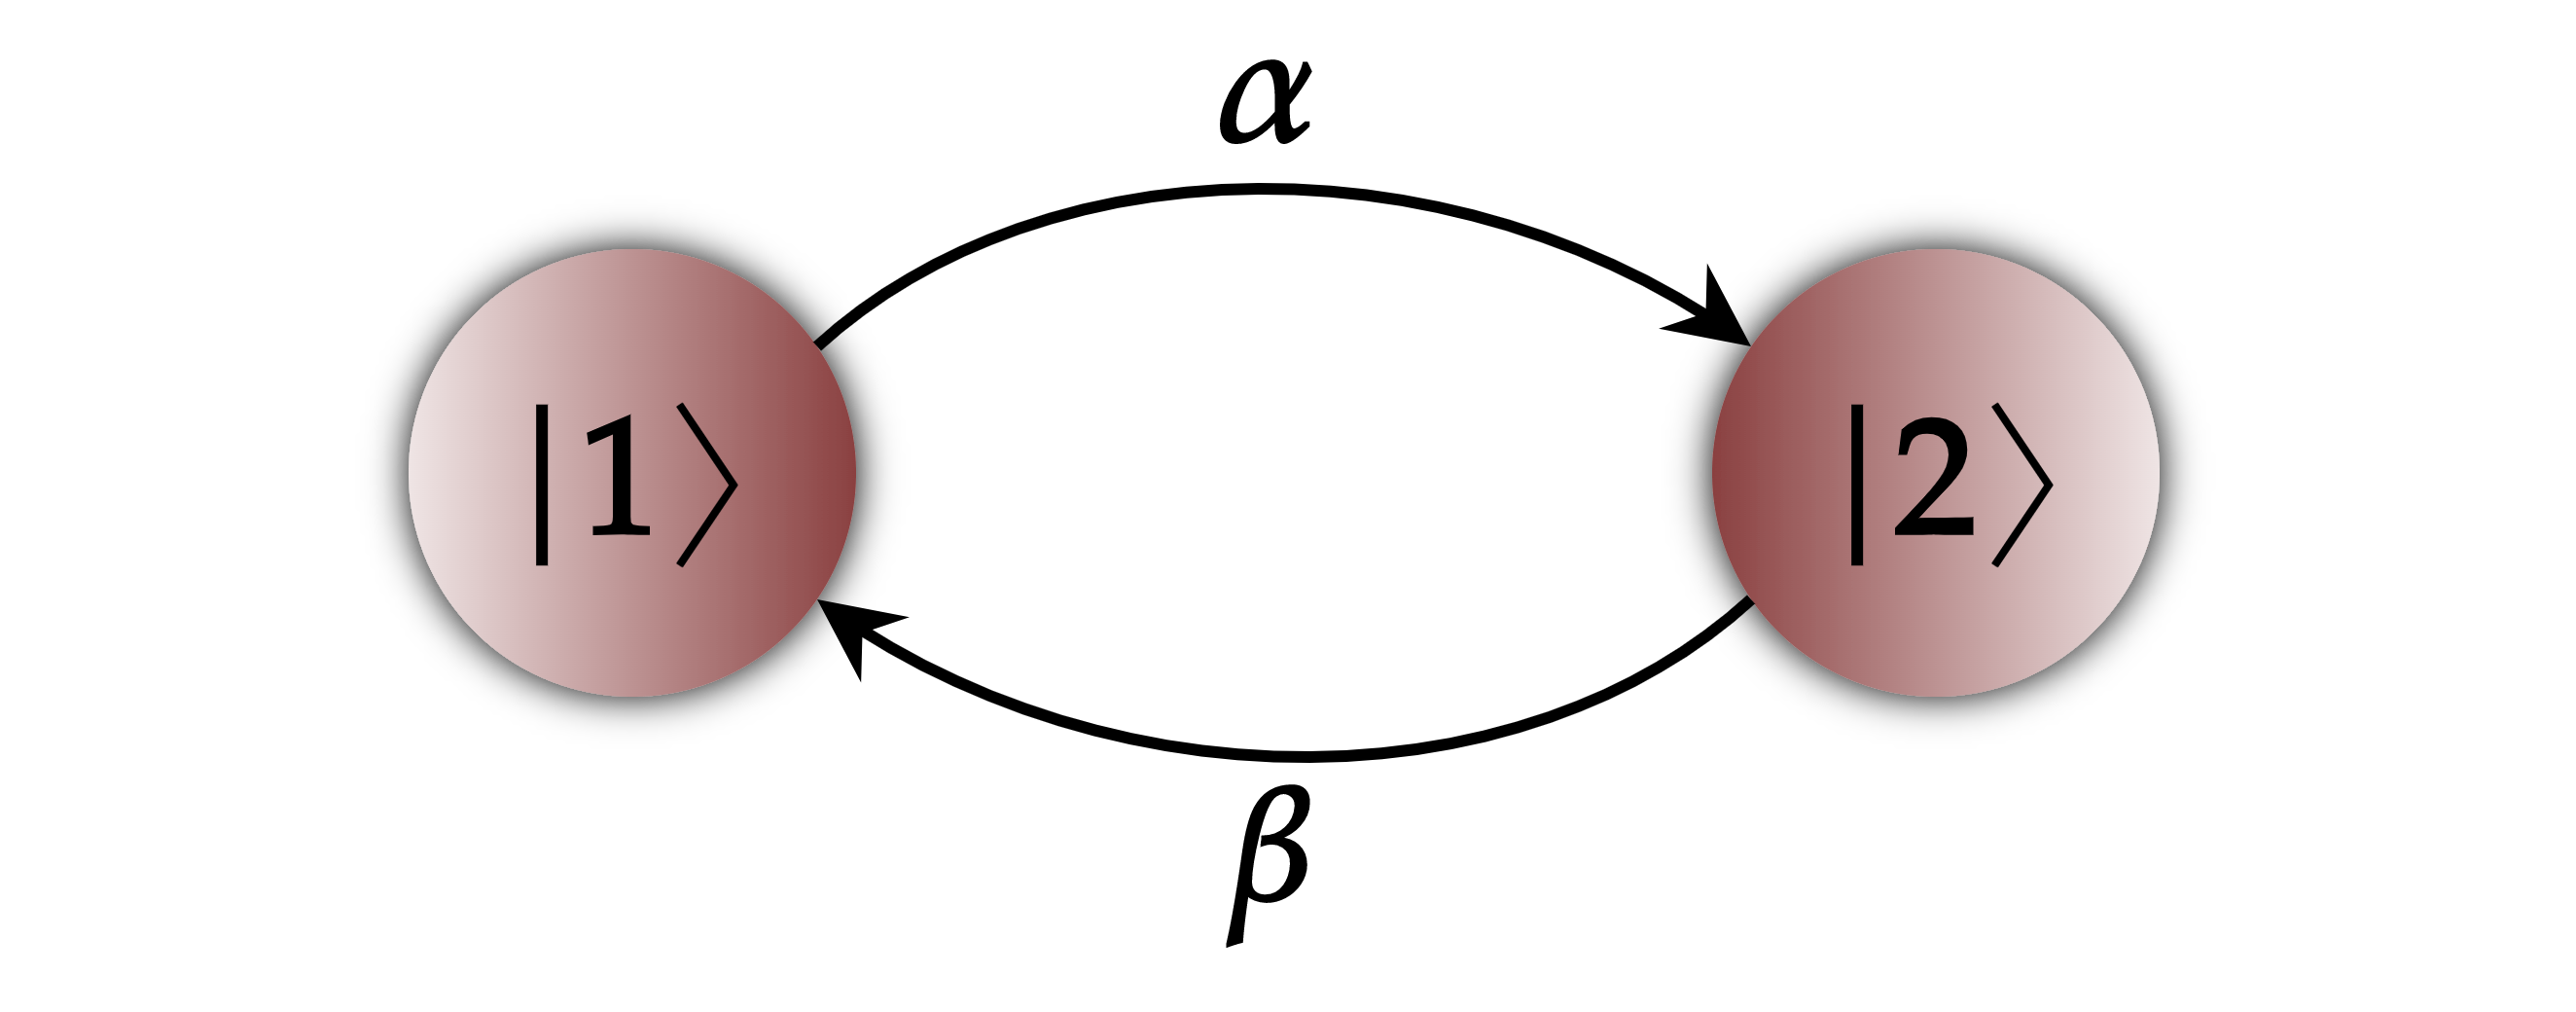
\includegraphics[width = 0.35\textwidth]{figures/tele-diagram-3.png}
\caption{\footnotesize Diagram of the telegraph process as described by Eqn. (\ref{two_state_transition_mat}). Regardless of the choice of initial condition, this system will settle into the equilibrium distribution $P(t) = \frac{1}{\alpha +\beta}(\beta\ket{1} + \alpha \ket{2})$. In this distribution the detailed balance conditions is satisfied, hence $\entpp = 0$ in the long-time limit.} 
\label{telegraph-diagram}
\end{wrapfigure}

The telegraph process is the continuous-time, two-state Markov chain described by the master equation

\begin{align}\label{two_state_transition_mat}
  \dot{P}(t) = P(t)e^{tW}, \; \; \; W = \begin{pmatrix}-\alpha && \alpha \\ \beta && -\beta \end{pmatrix}.
\end{align}


The telegraph process is a building block of more complicated processes which we will consider later in this text. For this reason, it is helpful to review some known results about its entropy production rate. Although the entropy production of discrete state-space Markov chains is usually considered from the stand point of graph theory, here we will replicate these results using a path-space formulation of entropy production. In this way we will develop some useful results by considering this simple system. This simple system will also provide a first stress test for our original framework for the derivation of path probabilities that we plan to use throughout much of this thesis. 

We will label the two states $\ket{1} $ and $\ket{2}$. We shall use the terms `particle' and `system' interchangeably, i.e. we may speak of the system or the particle being in state $\ket{1}$ etc. Given an initial condition $P(0) = P_0 = p\ket{1}  + (1-p)\ket{2} $, the system will evolve according to $P(t) = e^{tW}P_0$, and it will eventually reach the equilibrium distribution $P_\infty$, which is the normalised eigenvector of $e^{tW}$ with eigenvalue equal to one. Indeed

\begin{equation}\label{telegraph-state-prob}
  P(t) = A(t)\ket{1}  + B(t)\ket{2}  = \frac{1}{\alpha + \beta} \left((\beta + re^{-(\alpha + \beta)t})\ket{1}  +
(\alpha - re^{-(\alpha + \beta)t})\ket{2}  \right) ,
\end{equation}

with $r = \alpha p - \beta(1-p)$. The entropy productions rate of the telegraph process is then given by  \cite{cocconi2020entropy}

\begin{align}\label{telegraph-entropy-Luca}
  \entpp(t) &= re^{-(\alpha + \beta)t}\log \left(\frac{1+\frac{r}{\beta}e^{-(\alpha + \beta)t}}{1-\frac{r}{\alpha}e^{-(\alpha + \beta)t}}\right).
\end{align}


 The most immediate observation from this result is that the entropy production rate of the telegraph process converges exponentially to zero. This is consistent with the fact that at its stationary state the telegraph process obeys the detailed balance condition, so it does not allow any current. Markov processes with null current cannot produce any entropy. The exponential decay of the entropy production rate also reflects the exponential decay of the initial state to statistical equilibrium. Note the non-negativity of $\entpp$ for all choices of $\alpha$,$\beta$, and $t$. 

 In the following section we will recover (\ref{telegraph-state-prob}) and (\ref{telegraph-entropy-Luca}) through a novel path-space formulation. While recovering these results through a path-space formulation proves much more difficult than their original derivation through a state-space description, the path-space formulation will eventually allow us to deal with coarse-grained non-Markov systems that are not responsive to classical treatments.

\subsection{Path Probabilities}\label{two_state_path_prob}

Consider the discrete time, two-state Markov chain that evolves according to the matrix

\begin{equation}
M = \mathds{1} + \frac{t}{N}W, \; \; N \in \mathds{N},
\end{equation}

with $W$ as in (\ref{two_state_transition_mat}). This is the discretised analogue of the process described by (\ref{two_state_transition_mat}). The choice of $M$ as the stochastic matrix for this process is motivated by Proposition \ref{limit-of-mat} which states that\footnote{See Appendix A for an amusing proof of this proposition.}

\begin{align}
\lim_{N\rightarrow \infty}M^N = e^{tW}.
\end{align}

In the language of stochastic processes, $W$ is the generator of the Markov chain described by $M$. 

We prepare the system in $\ket{1}$, i.e. $p=1$. Then, given that the system starts in state $\ket{1} $, the probability of finding it there again after time $t/N$, having made no jumps, is given by $\bra{1} M\ket{1}  $. Moreover, the probability of the system making no jumps in time $t = Nt/N$ is

\begin{equation}
  \underbrace{\bra{1} M\ket{1}  \bra{1} M\ket{1}  \ldots \bra{1} M\ket{1}  }_{N \; \text{inner products}} = \left(1+\frac{tW_{11}}{N}\right)^N
\end{equation}

To find the probability of the constant path $\omega_0$ (the unique path which begins and ends in $\ket{1}  $, with no jumps in time $t$), we take the limit of $N \rightarrow \infty$ to find

\begin{equation}
  \bP(\omega_0) = \lim_{N \rightarrow \infty} \left(1+\frac{tW_{11}}{N}\right)^N = e^{-\alpha t}
\end{equation}

On the other hand, the probability of a path $\omega_1$ that makes only one jump to state $\ket{2}  $ and at time $t_1 > 0$ is given by

\begin{equation}\label{omega1_prob}
  \bP(\omega_1) = \lim_{N \rightarrow \infty}\left ( \underbrace{\bra{1} M\ket{1}  \ldots \bra{1} M\ket{1}  }_{N_1 \; \text{inner products}} \overbrace{\bra{1} M \ket{2}  }^{ = \frac{\alpha t}{N}} \underbrace {\bra{2} M\ket{2}  \ldots \bra{2} M\ket{2}  }_{N - N_1 \; \text{inner products}}\right)
\end{equation}

In the above, $t_1 = N_1t/N$. Now if let $N$ go to infinity while fixing $N_1/N = t_1/t$, this will ensures that $N_1$ is large. Note also that

$$\lim_{N \rightarrow \infty} (1+ \frac{x}{N})^{c N} = (e^x)^c = e^{c x}$$

We let $t/N \rightarrow \rmd t_1 $ as $N \rightarrow \infty$.\footnote{To make a rigorous argument for why $t/N \rightarrow \rmd t_1$ we would simply have to index the time steps. Then we note that moving the transition one step to the right (left) adds (subtracts) an increment of size $t/N$ to the time $t_1$.}  Also let $\Omega_1 \subset \Omega$ be the subset of all paths that make only one transition in time $t$. Then the limit of Equation \ref{omega1_prob} is the density $\bP\lvert_{\Omega_1}$.

\begin{align}
  \bP(\omega \in \Omega_1 ) &= \lim_{N \rightarrow \infty}\left [ \left(1 + \frac{tW_{11}}{N}\right)^{\frac{Nt_1}{t}} \frac{\alpha t}{N}  \left(1+\frac{tW_{22}}{N}\right)^{\frac{N(t-t_1)}{t}} \right ] \\
  &= \alpha e^{-\alpha t\frac{t_1}{t}}e^{-\beta t \frac{(t-t_1)}{t}}\rmd t_1 = \alpha e^{-\alpha t_1}e^{-\beta (t-t_1)} \rmd t_1
\end{align}

Let now $\Omega_L \subset \Omega$ be the subset of paths that make $L$ jumps at times $t_i$ . We can similarly calculate the density of $\bP$ on $\Omega_2$ to be

\begin{equation}
  \bP(\omega \in \Omega_2) = \alpha \beta e^{-\alpha t_1}e^{-\beta (t_2 - t_1)}e^{-\alpha (t-t_2)} \rmd t_1\rmd t_2.
\end{equation}

More generally, the density of $\bP|_{\Omega_L}$ is

\begin{equation}\label{density_omega_L}
  \bP(\omega \in \Omega_L) = \alpha^n\beta^m  \prod_{i =0, \:\text{even}}^{L} e^{-\alpha(t_{i+1} - t_{i})}\rmd t_i \prod_{i \: \text{odd}}^L e^{-\beta(t_{i+1} - t_{i})} \rmd t_i; \; \; t_0 = 0, \; t_{L+1} = t.
\end{equation}

In Equation \ref{density_omega_L}, $n$ is the number of transitions of the kind $\ket{1} \rightarrow \ket{2}$, while $m$ is the number of transitions of the kind $\ket{2} \rightarrow \ket{1}$. Clearly $n+m = L$. Notice that if $L$ is even, then the particle ends up back at $\ket{1}$ by time $t$, hence $n - m = 0$. Otherwise if $L$ is odd, then the system is in state $\ket{2}$ at time $t$, so $n-m = 1$. $t_i$ being the time of the $i$-th jump, we must have $t_i \in (t, t_{i-1})$. Furthermore, since the particle's jumps occur instantaneously, and the lower bound on the time between two jumps is zero, the number of jumps does not impose any additional constraints on the $t_i$'s.

\subsection{Recovering the Probability Flow}
To validate our approach, we will use these path probabilities to recover the probability time evolutions $A(t)$ and $B(t)$ as in Equation (\ref{telegraph-state-prob}. We begin by finding a convenient analytical expression for the probability $\bP(\Omega_L)$. The probability of $\Omega_L$ is

\begin{equation}\label{Omega_L_prob}
  \bP(\Omega_L) = \alpha^n\beta^m  \int^{t}_{0}\rmd t_1\int^{t}_{t_1}\rmd t_2\ldots \int^{t}_{t_{L-1}}\rmd t_L\prod_{i =0, \:\text{even}}^{L} e^{-\alpha(t_{i+1} - t_{i})} \prod_{i \: \text{odd}}^L e^{-\beta(t_{i+1} - t_{i})}.
\end{equation}

Let us first examine this quantity in the case where $\alpha = \beta$. In such an instance Equation \ref{Omega_L_prob} takes the much simpler form

\begin{equation}\label{alpha_eq_beta}
  \bP(\Omega_L | \alpha = \beta) = \alpha^L e^{-\alpha t}  \int^{t}_{0}\rmd t_1\int^{t}_{t_1}\rmd t_2\ldots \int^{t}_{t_{L-1}}\rmd t_L = \frac{(\alpha t)^L}{L!}e^{-\alpha t}.
\end{equation}

We find that in the case where $\alpha = \beta$ the system reduces to a simple Poisson counting process with parameter $\lambda = \alpha t$. To treat the general case, first notice that \ref{Omega_L_prob} may be written

\begin{equation}
\bP(\Omega_L) = \alpha^n\beta^m e^{-\beta t} \int_0^t e^{(\beta - \alpha)t_1}\rmd t_1\int_{t_1}^t e^{(\alpha -\beta)t_2}\rmd t_2\ldots \int_{t_{L-1}}^t e^{(\beta - \alpha)t_L}\rmd t_L,
\end{equation}

where we have assumed that $L$ is odd. If $L$ were even, then we would only replace the integrand of the right most integral with $e^{(\alpha -\beta)t_L}$ and also replace the prefactor $e^{-\beta t}$ with $e^{-\alpha t}$. For $n = 0,1,2, \ldots$, let $I_n(t,r)$ be the integral 



 \begin{align}
    I_n(t,r)= \int_0^t \rmd t_1\int_{t_1}^t \rmd t_2\ldots \int_{t_{L-1}}^t \rmd t_n \prod_{i \; \text{odd}}^n e^{rt_i} \prod_{i \: \text{even}}^n e^{-rt_i},
 \end{align}

 with the convention $I_0 = 1$. Then we have
  
 \begin{align}
  \bP(\Omega_L) =  \begin{cases}   \alpha^{L/2}\beta^{L/2}e^{-\alpha t}I_L(t,\beta - \alpha), & \text{$L$ even}\\
  & \\
  \alpha^{(L+1)/2}\beta^{(L-1)/2}e^{-\beta t}I_L(t,\beta - \alpha), & \text{$L$ odd}.
  \end{cases}
 \end{align}
  
Now, by Proposition \ref{recursion-lemma}, we have the recursion relations 

  \begin{align}\label{differential_recurrence_odd}
    \dot{I}_{n+1}(t,r) = e^{-rt}  I_n(t,r); \; \; I_{n+1}(0,r) = 0,
  \end{align}

  for odd $n$ and

  \begin{align}\label{differential_recurrence_even}
    \dot{I}_{n+1}(t,r) = e^{rt}  I_n(t,r); \; \; I_{n+1}(0,r) = 0.
  \end{align}

  for even $n$.


Taking the Laplace transform of (\ref{differential_recurrence_odd}) and (\ref{differential_recurrence_even}), we obtain


\begin{align}
\begin{split}
\tilde{I}_{n+1}(s) &= \frac{\tilde{I}_n(s+r)}{s}, \hspace{20pt} \text{$n$ odd} \\
\tilde{I}_{n+1}(s) &= \frac{\tilde{I}_n(s-r)}{s}, \hspace{20pt} \text{$n$ even}.
\end{split}
\end{align}

Here $\tilde{f}(s)$ denotes the Laplace transform of $f(t)$. Applying this relation recursively we have 

\begin{align}
\begin{split}
\tilde{I}_2(s) =& \frac{\tilde{I}_0(s)}{s(s+r)}\\
\tilde{I}_4(s) =& \frac{\tilde{I}_0(s)}{s^2(s+r)^2}\\
\tilde{I}_6(s) =& \frac{\tilde{I}_0(s)}{s^3(s+r)^3}\\
&\vdots
\end{split}
\quad\quad
\begin{split}
\tilde{I}_3(s) =& \frac{\tilde{I}_1(s)}{s(s-r)}\\
\tilde{I}_5(s) =& \frac{\tilde{I}_1(s)}{s^2(s-r)^2}\\
\tilde{I}_7(s) =& \frac{\tilde{I}_1(s)}{s^3(s-r)^3}\\
&\vdots
\end{split}
\end{align}

whence we derive the expressions 

\begin{align}\label{inverse_laplace_int}
\begin{split}
I_{2n}(t,r) &= \mathcal{L}^{-1}\left [ \frac {\tilde{I}_0(s)}{s^n(s+r)^n}\right](t) =\mathcal{L}^{-1}\left [ \frac {1/s}{s^n(s+r)^n}\right](t) , \\
I_{2n+1}(t,r) &= \mathcal{L}^{-1}\left [ \frac {\tilde{I}_1(s)}{s^n(s-r)^n}\right](t) = \frac{1}{r}\mathcal{L}^{-1}\left [ \frac {1/(s-r)-1/s}{s^n(s-r)^n}\right](t).
\end{split}
\end{align}

Computationally, evaluating (\ref{inverse_laplace_int}) is a matter of partial fraction decomposition. The required inverse Laplace transform can subsequently be read off from a look-up table. In fact, the inverse Laplace transform can be calculated in each case to be 
\begin{align}
    I_{2n}(t,r) &= \frac{e^{-rt/2}(t/r)^n\sqrt{\pi rt}}{2n!}\left (B_{n-\frac{1}{2}}\left(\frac{rt}{2}\right) + B_{n+\frac{1}{2}}\left(\frac{rt}{2}\right)\right)\\
    I_{2n+1}(t,r) &= \frac{e^{-rt/2}(t/r)^n\sqrt{\pi rt}B_{n+\frac{1}{2}}\left(\frac{rt}{2}\right)}{2n!},
\end{align}

where $B_\nu(z)$ is the modified Bessel function of the first kind and $\Gamma(z)$ is the gamma function

\begin{align}
\Gamma(z) = \int_0^\infty t^{1-z}e^{-t}\:\rmd t, \; \; \; \mathcal{R}(z) > 0. 
\end{align}

The simple form of (\ref{inverse_laplace_int}) will also allow us to sum the $\bP(\Omega_L)$ in Laplace space to recover the normalisation 

\begin{equation}
\sum_{L = 0}^\infty \bP(\Omega_L) = 1.
\end{equation}

Consider first the sum of $\bP(\Omega_L)$ for even $L$. We have 

\begin{align}
\begin{split}
\sum_{l = 0}^\infty \bP(\Omega_{2l}) &= \sum_{l=0}^\infty \alpha^l\beta^le^{-\alpha t}I_{2l}(t, \beta -\alpha)\\
&= e^{-\alpha t}\sum_{l=0}^\infty (\alpha \beta)^l\mathcal{L}^{-1}\left [ \frac {\tilde{I}_0(s)}{s^l(s+\beta-\alpha)^l}\right](t) \\ 
&= e^{-\alpha t}\mathcal{L}^{-1}\left \{ \frac{1}{s}\sum_{l=0}^\infty\frac{(\alpha\beta)^l}{s^l(s+\beta-\alpha)^l}\right\}(t)\\
&= e^{-\alpha t}\mathcal{L}^{-1}\left \{\frac{s+\beta - \alpha}{s^2 +(\beta - \alpha)s-\alpha\beta} \right\}(t)\\
&= \frac{\beta + \alpha e^{-(\alpha + \beta)t}}{\alpha + \beta} = A(t)|_{p=1},
\end{split}
\end{align}

where we have used the fact that $I_0(s) \equiv 1$ and $\mathcal{L}[1](s) = 1/s$. Hence we have recovered $A(t)$ from (\ref{telegraph-state-prob}). Indeed, the sum of probabilities of all paths with an even number of transitions starting from $\ket{1}$ is precisely the probability that the particle will be in state $\ket{1}$ after time $t$, i.e. $A(t)$ evaluated at $p=1$. A similar calculation yields
\begin{align}
\begin{split}\label{odd-normalisation}
\sum_{l=0}^\infty \bP\left(\Omega_{2l+1}\right) &= \sum_{L=0}^\infty \alpha^{(2l+1+1)/2}\beta^{(2l+1-1)/2}e^{-\beta t}I_{2l+1}(t,\beta - \alpha)\\ 
&= \alpha e^{-\beta t} \sum_{l = 0 }^\infty (\alpha\beta)^l\mathcal{L}^{-1}\left [ \frac {\tilde{I}_1(s)}{s^n(s-\beta +\alpha)^n}\right](t) \\ 
&= \frac{\alpha}{\alpha + \beta}(1-e^{-(\alpha +\beta)t}) = B(t)|_{p=1}, 
\end{split}
\end{align}

for the sum of $\bP(\Omega_L)$ with odd $L$. Hence, we recover the normalisation

\begin{align}
    \sum_{l = 0}^\infty \bP(\Omega_l)= \frac{\beta + \alpha e^{-(\alpha+\beta)t}}{\alpha + \beta} + \frac{\alpha}{\alpha + \beta}(1-e^{-(\alpha +\beta)t}) = 1.
\end{align}

\subsection{Entropy Production}

Let us consider the telegraph process with initial distribution $P(0) = p\ket{1} + (1-p)\ket{2}$ where $0 < p < 1$. In the foregoing section, $\Omega$ was used to denote all paths of the telegraph process beginning from $\ket{1}$. We will now recycle this notation and let $\Omega$ denote all possible paths for the telegraph process in time $t$, regardless of starting position. We also introduce the following subsets of $\Omega$ 

\begin{align}
    \begin{split}
    \Omega_L^1 = \{ \omega: \:\text{$\omega$ starts at $\ket{1}$ and makes $L$ transitions} \}, \\ 
    \Omega_L^2 = \{ \omega: \:\text{$\omega$ starts at $\ket{2}$ and makes $L$ transitions} \},
    \end{split}
\end{align}

for $L = 0, 1, 2, \ldots$. Let $\omega^\ast$ denote the time-reversed realisation of $\omega$. If $\omega \in \Omega_L^i$, and $L$ is even, then $\omega$ ends in state $\ket{i}$. Hence the time-reverse $\omega^\ast$ also begins at $\ket{i}$ and makes $L$ transitions, so $\omega^\ast \in \Omega^i_L$. If instead $L$ is odd, then $\omega \in \Omega^i_L$ ends in the opposite state $\ket{j}$, therefore $\omega^\ast \in \Omega^j_L$. Let $\bP$ be the measure the measure on $\Omega$ at time $s=0$, and $\bP_\ast$ the measure at $s = t$. In other words $\bP$ is the path-space measure given the initial condition $P(0)$, while $\bP_\ast$ is the path-space measure given the initial condition $P(t)$ (see the discussion on entropy production in \ref{subsection:entropy-prod-discussion}). For $L$ even and $\ket{i} = \ket{1}$, we have the probabilities

\begin{align}
\begin{split}
\bP(\omega \in \Omega_L^1) &= p\rmd t_1 \ldots \rmd t_L \alpha^{L/2}\beta^{L/2}e^{-\alpha t}I_L(t,\beta - \alpha),\\
\bP_\ast(\omega \in \Omega_L^1) &= A(t) \rmd t_1 \ldots \rmd t_L \alpha^{L/2}\beta^{L/2}e^{-\alpha t}I_L(t,\beta - \alpha).
\end{split}
\end{align}

This follows from the equality 

\begin{align}
\begin{split}
\bP(\omega \in \Omega_L^1) &= \bP(\text{$\omega$ begins in $\ket{1}$}, \: \text{$\omega$ makes $L$ transitions})\\
&= \bP(\text{$\omega$ begins in $\ket{1}$})\bP(\text{$\omega$ makes $L$ transitions} \: |\: \text{$\omega$ begins in $\ket{1}$})
\end{split}
\end{align}

and similar for $\bP_\ast$. Similar calculations show that 

\begin{align}
\bP(\omega \in \Omega^i_L) &=\rmd t_1 \ldots \rmd t_L \begin{cases}p\alpha^{L/2}\beta^{L/2}e^{-\alpha t}I_L(t,\beta - \alpha) & \text{$L$ even,i = 1}\\ 
p\alpha^{(L+1)/2}\beta^{(L-1)/2}e^{-\beta t}I_L(t,\beta - \alpha) & \text{$L$ odd,\:$i = 1$} \\ 
(1-p)\alpha^{L/2}\beta^{L/2}e^{-\beta t}I_L(t,\alpha - \beta) & \text{$L$ even,\:$i = 2$}\\ 
(1-p)\alpha^{(L-1)/2}\beta^{(L+1)/2}e^{-\alpha t}I_L(t,\alpha - \beta) & \text{$L$ odd,\:$i = 2$},\end{cases} \\ 
\bP_\ast(\omega \in \Omega^i_L) &=\rmd t_1 \ldots \rmd t_L \begin{cases}A(t)\alpha^{L/2}\beta^{L/2}e^{-\alpha t}I_L(t,\beta - \alpha) & \text{$L$ even,\:$i = 1$}\\ 
A(t)\alpha^{(L+1)/2}\beta^{(L-1)/2}e^{-\beta t}I_L(t,\beta - \alpha) & \text{$L$ odd,\:$i = 1$} \\ 
B(t)\alpha^{L/2}\beta^{L/2}e^{-\beta t}I_L(t,\alpha - \beta) & \text{$L$ even,\:$i = 2$}\\ 
B(t)\alpha^{(L-1)/2}\beta^{(L+1)/2}e^{-\alpha t}I_L(t,\alpha - \beta) & \text{$L$ odd,\:$i = 2$}.\end{cases}
\end{align}

If $L$ is even and $\omega \in \Omega^i_L$, then $\omega^\ast \in \Omega_L^i$ and we have 

\begin{align}\label{prob-ratio-even}
\frac{\bP(\omega \in \Omega^i_L)}{\bP_\ast(\omega^\ast \in \Omega^i_L)} = \begin{cases}p/A(t), & i = 1 \\ (1-p)/B(t), & i=2.\end{cases}
\end{align}

If $L$ is odd, then $\omega$ and $\omega^\ast$ begin in different states, and we have

\begin{align}\label{prob-ratio-odd}
\frac{\bP(\omega \in \Omega^i_L)}{\bP_\ast(\omega^\ast \in \Omega^j_L)} = \begin{cases}\frac{\alpha pI_L(t,\beta - \alpha)}{\beta B(t)I_L(t,\alpha - \beta)}e^{(\alpha - \beta)t} & i = 1, \: j = 2, \\ 
\frac{\beta(1-p) I_L(t,\alpha - \beta)}{\alpha A(t) I_L(t,\beta - \alpha)}e^{(\beta - \alpha)t}& i=2, \: j=1.\end{cases}
\end{align}

Now, from previous calculations we have that 

\begin{align}\label{explicit-integral-bessel}
I_{2n+1}(t,r) = \frac{1}{r}\mathcal{L}^{-1}\left [ \frac {1/(s-r)-1/s}{s^n(s-r)^n}\right](t) = \frac{e^{rt/2}}{n!}\left(\frac{t^2}{2}\right)^{n+1/2}\sum_{k=0}^{\infty}\frac{(\frac{1}{2}rt)^{2k}}{k!\Gamma(n+k+\frac{3}{2})},
\end{align}


Since the sum in (\ref{explicit-integral-bessel}) is even in $r$, we conclude that 

\begin{align}
\frac{I_L(t,r)}{I_L(t,-r)} = e^{rt}, \; \; \; \text{$L$ odd},
\end{align}

whence the ratio in (\ref{prob-ratio-odd}) becomes 

\begin{align}
\frac{\bP(\omega \in \Omega^i_L)}{\bP_\ast(\omega^\ast \in \Omega^j_L)} = \begin{cases}\frac{\alpha p}{\beta B(t)} & i = 1, \: j = 2, \\ 
\frac{\beta(1-p)}{\alpha A(t)}& i=2, \: j=1.\end{cases}
\end{align}

Comparing this to (\ref{prob-ratio-even}) we note that in the case of even number of jumps, the only contribution to the entropy production is the time evolution of the system distribution. Where there is an odd number of transitions, however, the current observed between the two states contributes to entropy production through the ratio $\alpha/\beta$. The Radon-Nykodym derivatives only depend  on the parity of the number of transitions $L$, and they are independent of the transition times $t_i$. Hence, taking the logarithms of these we obtain the conditional expectations 

\begin{align}
\bE\left [\log \frac{\bP(\omega)}{\bP(\omega^\ast)} \: \bigg\lvert \: \Omega_L^i  \right] = \begin{cases}\log\left(\frac{p}{A(t)}\right) & $i = 1$, \text{$L$ even},\\
\log\left(\frac{\alpha p}{\beta B(t)}\right) & $i = 1$, \text{$L$ odd},\\
\log\left(\frac{1-p}{B(t)}\right) & $i = 2$, \text{$L$ even}\\
\log\left(\frac{\beta(1-p)}{\alpha A(t)}\right) & $i = 2$, \text{$L$ odd},\end{cases}
\end{align}

whereby, using results from the previous section for $\bP(\Omega_i^L)$, a few lines of algebra yields 

\begin{align}
    \begin{split}
   \mathcal{S} &= \bE \left[ \log \frac{\bP(\omega)}{\bP(\omega^\ast)} \right]\\ &= \sum_{i, L} \bE\left [\log \frac{\bP(\omega)}{\bP(\omega^\ast)} \: \bigg\lvert \: \Omega_L^i  \right]\bP(\Omega^i_L) \\
    &= \frac{1}{\alpha +\beta}\bigg [ p\log\left(\frac{p}{A(t)}\right)(\beta + \alpha e^{-(\alpha + \beta)t}) +p\log\left(\frac{\alpha p}{\beta B(t)}\right)(\alpha - \alpha e^{-(\alpha + \beta)t)}) \\
    &\quad + (1-p)\log \left (\frac{1-p}{B(t)}\right)(\alpha + \beta e^{-(\alpha + \beta)t}) + (1-p)\log\left( \frac{\beta(1-p)}{\alpha A(t)}\right)(\beta -\beta e^{-(\alpha + \beta)t})\bigg].
    \end{split}
\end{align}

Finally, taking the derivative of $\mathcal{S}$ gives 

\begin{align}
\entpp = re^{-(\alpha + \beta)t}\log\left(\frac{1+\frac{r}{\beta}e^{-(\alpha + \beta)t}}{1-\frac{r}{\alpha}e^{-(\alpha + \beta)t}}\right),
\end{align}

where $r = \alpha p - \beta (1-p)$ as before. This is precisely the quantity quoted in Equation (\ref{telegraph-entropy-Luca}) and calculated in \cite{cocconi2020entropy} through classical (i.e. state-space) methods. 

\subsection{Discussion}
In the above we have shown that the entropy production rate of the telegraph process as calculated through our path-space framework is equal to the entropy production rate as calculated through a classical state-space approach. While analysis in the path-space formalism is much more involved, it has the important benefit that it can be applied to systems where trajectories have hidden degrees of freedom. We shall make use of this in the following section where we derive the entropy production of the `waiting room' system.  






% Consider a three state system, $i = 1,2, 3$, that is driven by the master equation 

% \begin{align}
% P(t) = P_0e^{tW},
% \end{align}

% with $W$ an appropriate generator. Suppose that in an experimental setup, the states $i=2,3$ are indistinguishable. This may be the case, for example, when state $i=1$ results in bioluminescence which can be detected, while states $2$ and $3$ do not result in detectable bioluminiscence. See Figure () for a cartoon of the system. More formally, one may say that if the state-space is $\mathcal{X} = \{ 1,2,3\}$, then in this setup the experimenter only has access to the $\sigma$-algebra  
% \begin{align} 
% \mathcal{F} = \left \{\phi, \mathcal{X}, \{1\}, \{2,3\}\right\}.
% \end{align}
% In this case, the appropriate quantity for the entropy production of the system is not that which is assigned to it by the Markov state-space formulation, since this formulation relies on information from the $\sigma$-algebra $2^{\mathcal{X}}$, which is not experimentally accessible. Instead, if $\Omega$ is the space of coarse-grained paths, 

% \begin{align}
% \Omega = \{ (x_0,x_1, \ldots): \text{$x_i$ is $\mathcal{F}$ measurable}\},
% \end{align}

% then the appropriate interpretation 
\section{The Waiting Room}\label{chapter:waiting-room}
\textit{In this section we apply the path-space framework developed in Section \ref{chapter:telegraph} to the `waiting room' system as described below. We obtain a closed form for the steady-state entropy production of this non-Markov process. This is the first instance of such a result for a non-Markov system.} 
\subsection{The System}



\begin{figure}
  \begin{subfigure}[b]{0.49\textwidth}
  \centering
  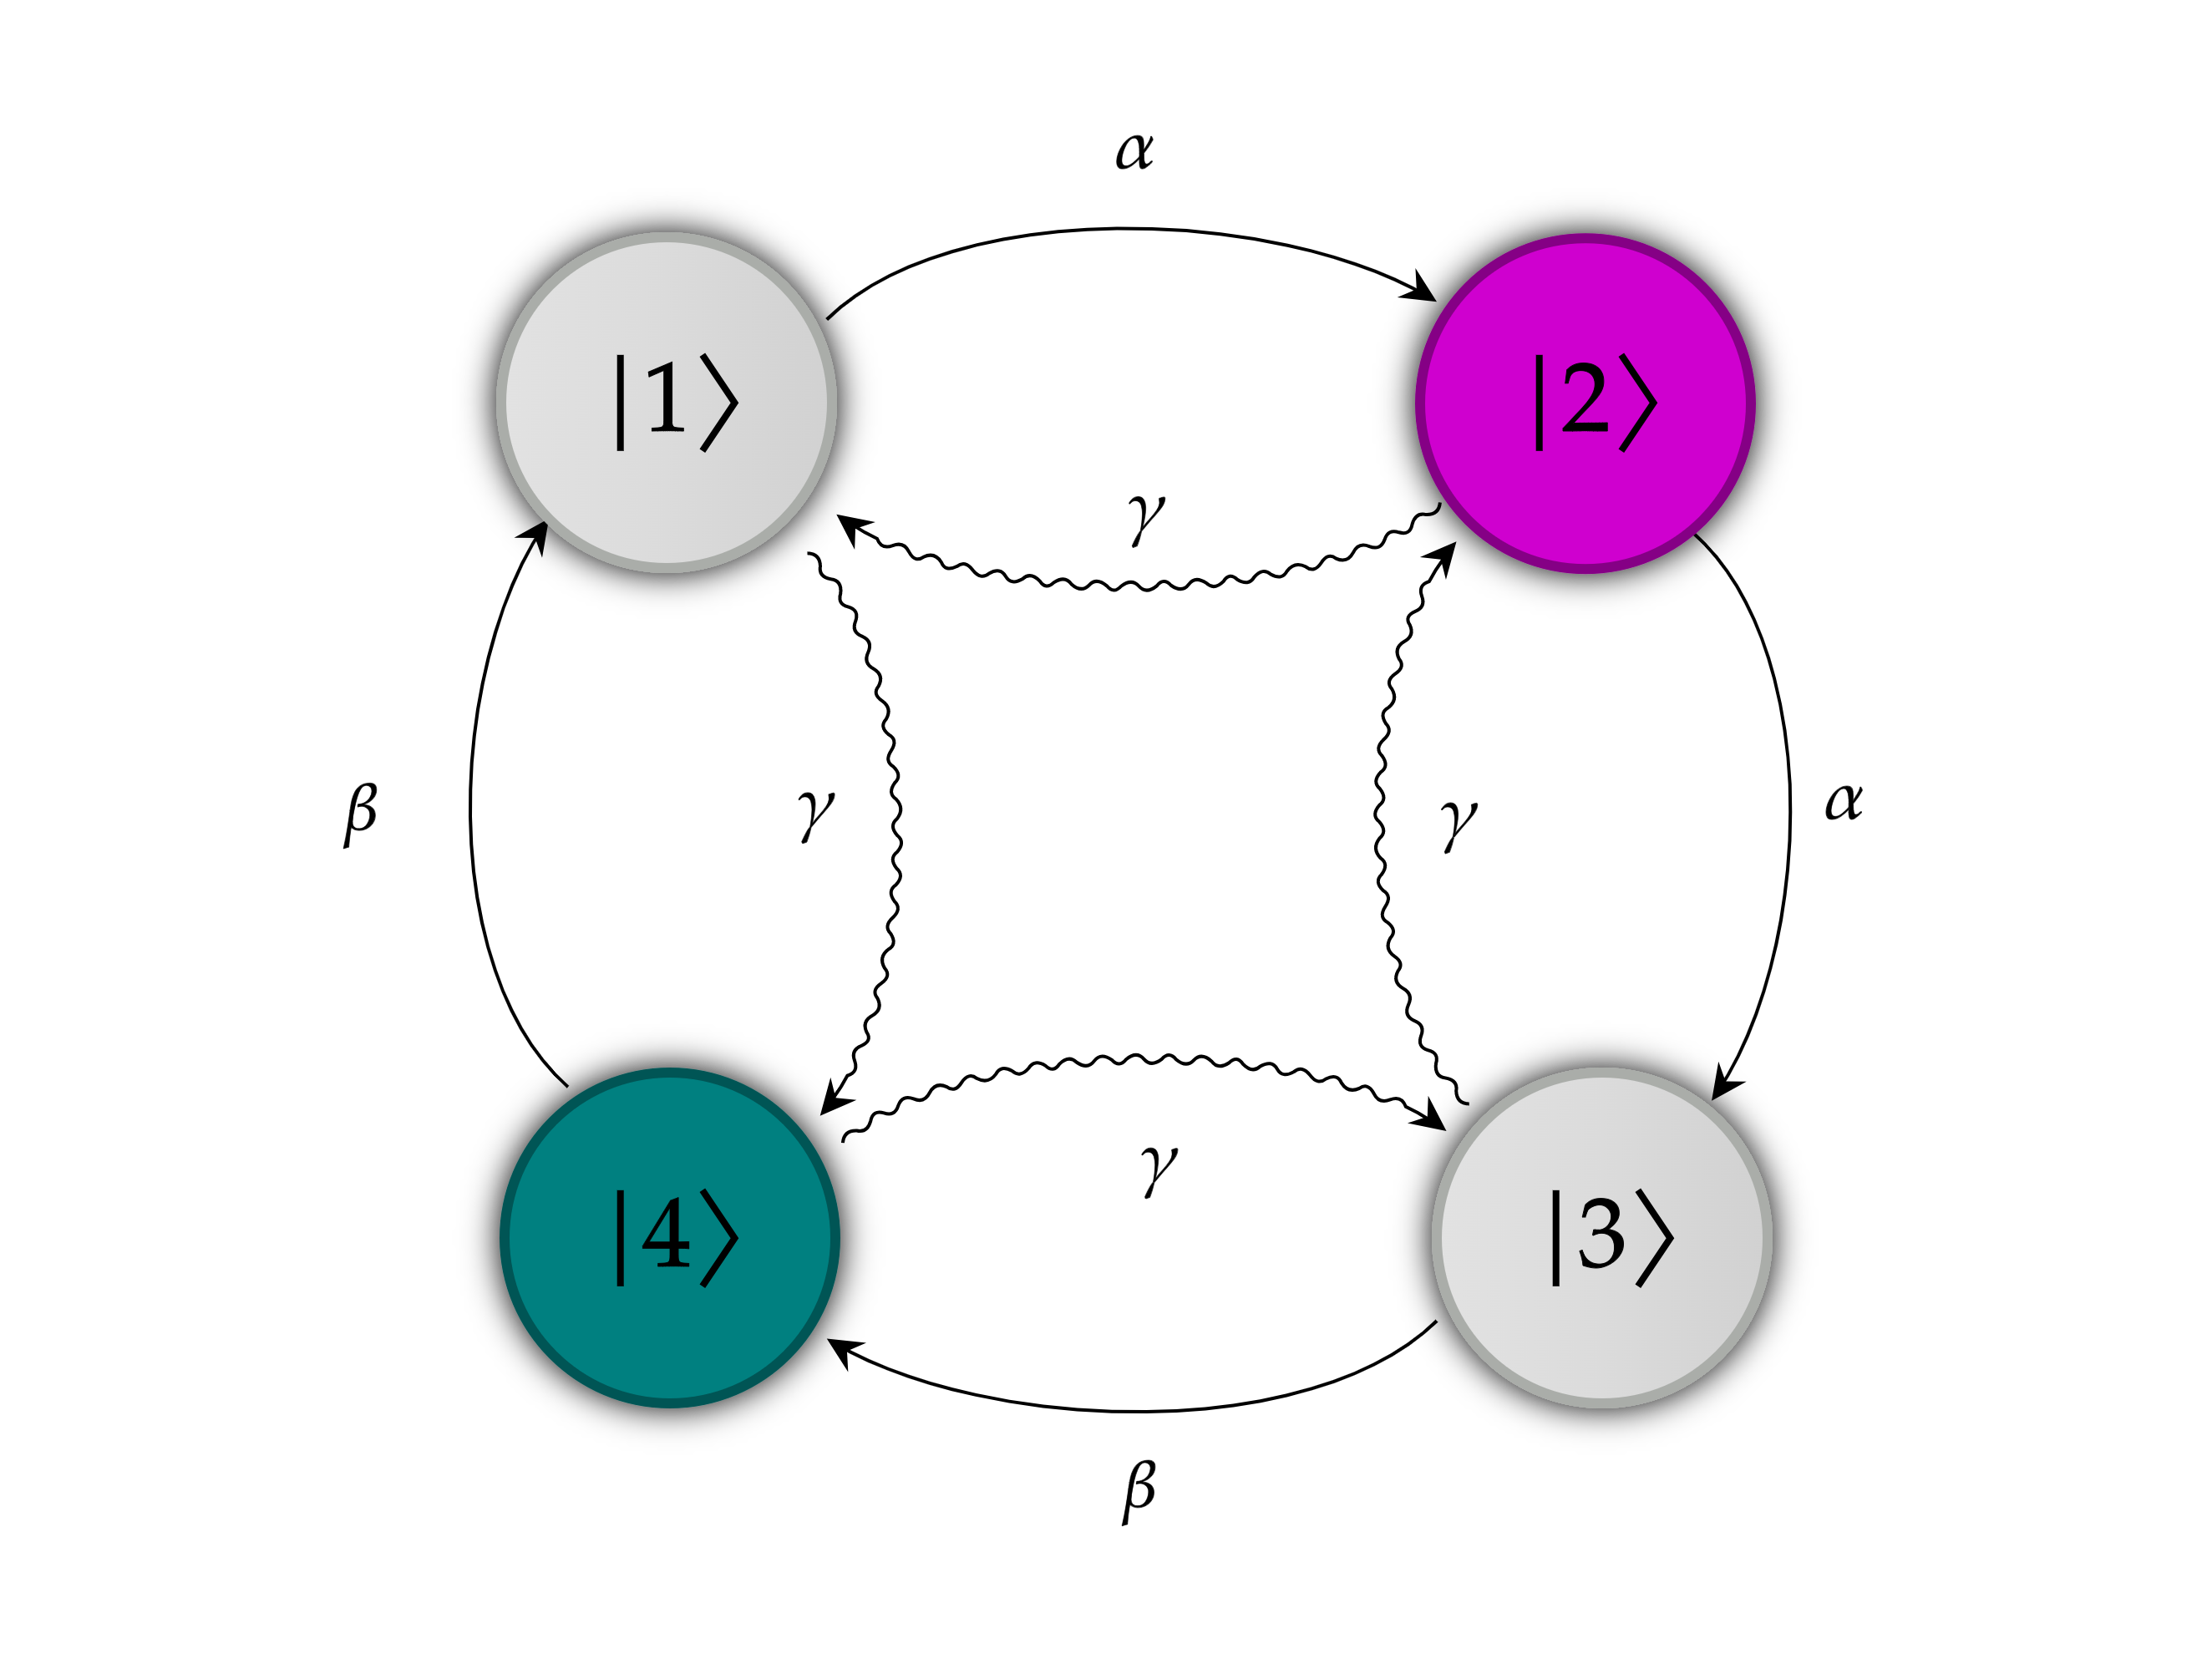
\includegraphics[width = \textwidth]{figures/waiting_room.png}
  \caption{Granular waiting room}
  \label{granular_fig}
\end{subfigure}
\begin{subfigure}[b]{0.49\textwidth}
  \centering
  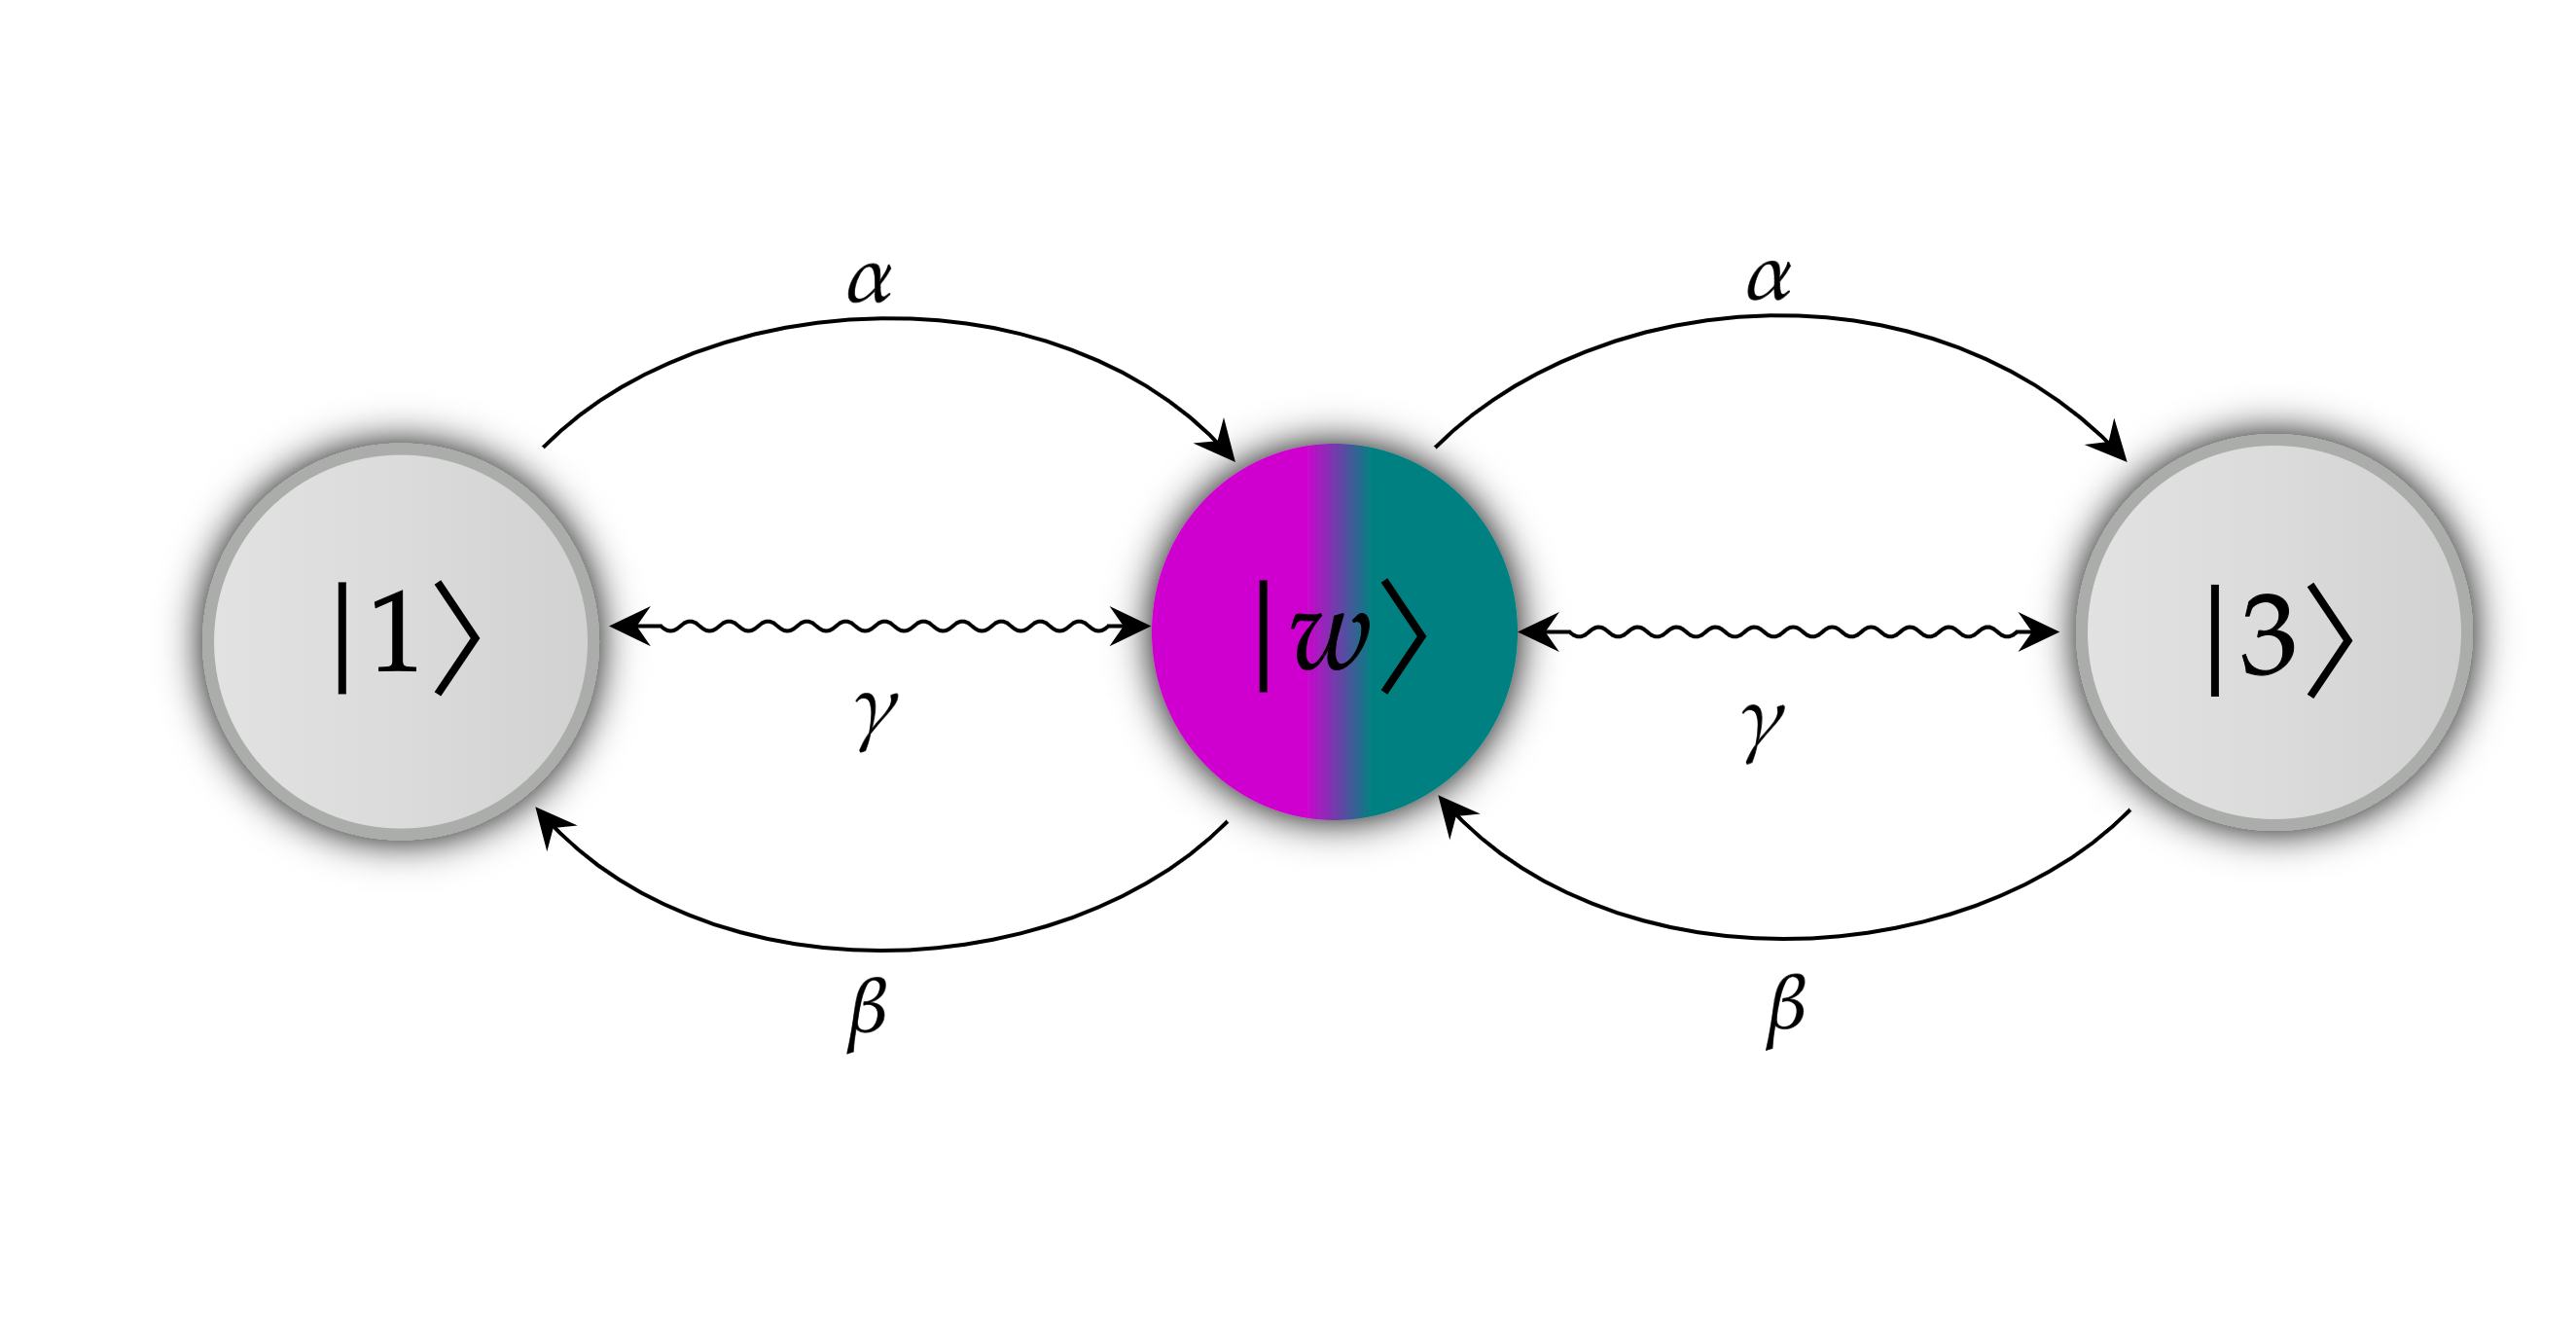
\includegraphics[width = \textwidth]{figures/wait_room_coarse.png}
  \caption{The waiting room}
  \label{coarse_grained_fig}
\end{subfigure}
\caption{\footnotesize Subfigure \ref{granular_fig} shows the granular Waiting Room (WR) system while \ref{coarse_grained_fig} shows the WR. Note that in the WR, there is no sense of cycle direction, i.e., to complete a cycle a particle must always traverse the state-space in the same order. This is in contrast to the granular WR where, starting from any state, a particle can cycle in the clockwise or anticlockwise directions. Depending on the values of the parameters $\alpha,\beta,$ and $\gamma$ this can lead to non-zero flux in the steady state of the granular WR. Meanwhile the WR cannot accommodate any net current in its steady state.}
\label{system_desc_fig}
\end{figure}

The system depicted in Figure \ref{granular_fig} is a Markov process with transition matrix

\begin{equation}
  W = W_{i \rightarrow j} = \begin{pmatrix}-\alpha - \gamma && \alpha && 0 && \gamma \\
\gamma && -\alpha - \gamma && \alpha && 0 \\
0 && \gamma && -\beta-\gamma && \beta \\
\beta && 0 && \gamma && -\beta - \gamma \end{pmatrix}.
\end{equation}

Henceforth we shall call this the granular `Waiting Room' (WR) system. As in Section \ref{two_state_path_prob}, it is possible to write down the density of paths around any given path by conditioning on the number of jumps made by a particle in the granular (WR) system. The added complication in this case is that the density will not only depend on the number of jumps, but also on the type of each jump (e.g. the density of paths making one jump of the type $\ket{1} \rightarrow \ket{2}$ is different to those making one jump of the type $\ket{1} \rightarrow \ket{4}$).

\begin{wrapfigure}{R}{0.4\textwidth}
    \centering
    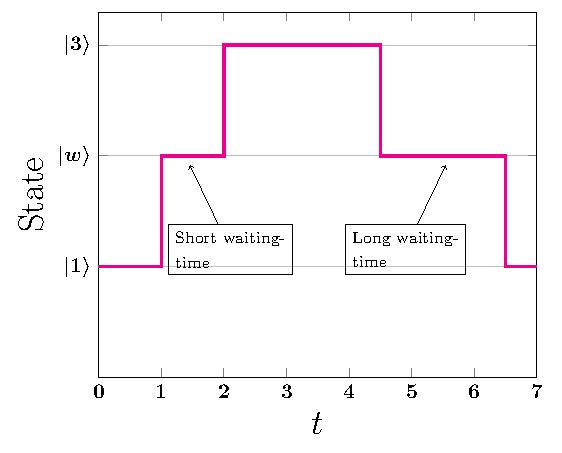
\includegraphics[width = 0.35\textwidth]{figures/waiting_room_sample_path.pdf}
    \caption{ \footnotesize A typical path for the WR system. For this path we assume $\alpha > \beta > \gamma$. The particle jumps from state $\ket{1}$ to $\ket{w}$ at $t = 1$ then to $\ket{3}$ at $t = 2$. It then climbs back down to $\ket{w}$ and eventually to $\ket{1}$. Since the system is much more likely to be in $\ket{2}$ if it has entered $\ket{w}$ from $\ket{1}$ (as it does at time $t = 1$), the expected waiting time in this case is much smaller than the case where the system enters $\ket{w}$ from $\ket{3}$ (as it does at $t = 4.5$), in which case it is most likely to have entered state $\ket{4}$ in the granular description. It is clear from this picture that the forward and reverse paths have different statistics.}
    \label{fig:coarse_grained_sample_path}
\end{wrapfigure}

From this granular WR system we obtain the WR system by collapsing the states $\ket{2}$ and $\ket{4}$ together as in Figure \ref{coarse_grained_fig}. The combination state obtained by this procedure we shall call $\ket{w}$. This coarse-grained system is no longer Markov since observed waiting times of the particle in $\ket{w}$ inform the inferred state of the system. It is also intuitively clear that the coarse-grained system has non-zero entropy production along its paths. See for example Figure \ref{fig:coarse_grained_sample_path} which shows a cartoon of a sample path. This cartoon makes evident the fact that the statistics of the forward and reverse paths are not equivalent. Our goal is to calculate the long-time expectation value for the Kullback-Leibler divergence of the coarse-grained paths. In doing so, we will assume that the system occupies its stationary state throughout. The most important implication of this assumption is that the time evolution of the measure of the process will no longer contribute to the entropy production as it did for the telegraph process in Section \ref{chapter:telegraph}. 

Each state in the granular system has an exponential waiting-time distribution $\psi_{\ket{i}}(t)$. This is distinct from the distribution of a transition $\ket{i} \rightarrow \ket{j}$ which we denote by $\psi_{ij}(t)$. The probability that a transition away from $\ket{i}$ is of the type $\ket{i} \rightarrow \ket{j}$ is then

\begin{equation}
    P_{ij} = \int_0^\infty \psi_{i j}(t)dt.
\end{equation}

The waiting time distribution conditioned on a given transition is then the normalised distribution $\psi_{ij}(t)/P_{ij}$. For example, using the methodology from Section II, we derive for state $\ket{1}$

\begin{align}
    \begin{split}
        \psi_{\ket{1}}(t) &= (\alpha + \gamma) e^{-(\alpha + \gamma)t},\\
        \psi_{12}(t) &= \alpha e^{-(\alpha + \gamma)t},\\
        \psi_{14}(t) &= \gamma e^{-(\alpha + \gamma)t},
    \end{split}
\end{align}

whereby $P_{12} = \frac{\alpha}{\alpha + \gamma}$, and $P_{14} = \frac{ \gamma}{ \alpha + \gamma}$ follow straightforwardly. Note that $\psi_{12}$ and $\psi_{14}$ are not normalised. The stationary distribution of the granular WR is given by 

\begin{align}\label{granular}
\begin{split}
\mu_1 &= \frac{1}{Z} \left(\alpha \alpha\beta^2 + \gamma(\beta^2 +\beta\gamma + \gamma^2) \right),\\
\mu_2 &= \frac{1}{Z}\left(\gamma^3 + \alpha(\beta^2 + \beta\gamma + \gamma^2)\right),\\ 
\mu_3 &= \frac{1}{Z}\left(\alpha\gamma^2 + \gamma^3 +\alpha^2(\beta+\gamma)\right),\\ 
\mu_4 &= \frac{1}{Z}\left(\alpha^2\beta +\alpha\beta\gamma+\gamma^2(\beta+\gamma)\right),\\
Z &= 2\alpha\beta(\alpha + \beta) +(\alpha+\beta)^2\gamma+2(\alpha+\beta)\gamma^2 +4\gamma^3.
\end{split}
\end{align}

The granular WR is a Markov chain, so we may calculate its steady-state entropy production rate according to \cite{schnakenberg1976network}

\begin{align}
\entpp_G = r\mathcal{A},
\end{align}

where $r$ is the \textit{clockwise} current of the system as seen in Figure \ref{granular_fig}, and 

\begin{align}
\mathcal{A} = \log\left (\frac{\alpha^2\beta^2}{\gamma^4}\right)
\end{align}

is the cycle affinity. Let $r_{ij} = r_{i \rightarrow j}$ be the current from $\ket{i}$ to $\ket{j}$. Then 
\begin{align}
r_{12} = \alpha \mu_1 - \gamma \mu_2 = \frac{1}{Z}(\alpha^2\beta^2-\gamma^2).
\end{align}
On the other hand, a simple application of Kirchoff's law yields, 
\begin{align}
r_{12} = r_{23} = r_{34} = r_{41},
\end{align}
hence $r = r_{12}/4$ and 
\begin{align}\label{granular-waiting-entropy-close}
\entpp^g = \frac{\alpha^2\beta^2-\gamma^4}{4Z}\log\left(\frac{\alpha^2\beta^2}{\gamma^4} \right).
\end{align}

We stress that in the WR, the state $\ket{w}$ does not indicate a particular combination state of $\ket{2}$ and $\ket{4}$, but any convex linear combination state $a\ket{2} + b\ket{4}$. The observer only has access to $\ket{w}$, but they may infer a probabilistic combination of $\ket{2}$ and $\ket{4}$ based on the system's history. In particular, if a state $\ket{\bar{w}} = a\ket{2} + b\ket{4}$ is inferred at $t = 0$, and the system has made no jumps in time $t$, then it occupies the combination state 

\begin{align}\label{waiting-room-timeevol}
\ket{\bar{w}(t)} = \frac{1}{a e^{-(\alpha + \gamma)t} + b e^{-(\beta + \gamma)t}}\left (a e^{-(\alpha + \gamma)t}\ket{2} + b e^{-(\beta + \gamma)t}  \ket{4}\right).
\end{align}

We may say that $\ket{w}$ is an \emph{observed} or observable state of the system, while $\ket{\bar{w}(t)}$ is an \emph{inferred} state.  

\subsection{Discrete Time Treatment}
\subsubsection{Path-Histories and Gluing Scheme}
\label{subsection:path-histories}

We will first treat this system in discrete time with time step $\tau$. Write $M = \mathds{1} + \tau W$ for the stochastic matrix of the discretised process. To avoid burdensome notation, we will write $(\ket{i}, m)$, for $i \in \{1, w, 3 \}$ and $m \in \bN \cup \{0\}$ to mean that the system was in state $\ket{i}$ for time $m\tau$. For any path $\omega$ beginning in $\ket{1}$ and ending in $\ket{3}$ the history of $\omega$ can be written

$$\{(\ket{1}, n_1), (\ket{w}, n_2), (\ket{3}, n_3), (\ket{w}, n_4), (\ket{1}, n_5), \ldots (\ket{3}, n_N)\}.$$

For example, if the path is given by $\omega = \ket{1}\xrightarrow{3}{} \ket{w} \xrightarrow{2}{} \ket{1} \xrightarrow{5}{} \ket{w} \xrightarrow{4}{} \ket{3}$ then we will have $n_1 = 3, n_2 =2, n_3 = n_4 = 0, n_5 = 5, n_6 = 4$.  Given a history in the form $\mathcal{P} = \{i_1, i_2, i_3, \ldots, i_N\}$ in the granular system, where the $i_k$ are states, we know that the probability of the path described by $\mathcal{P}$ is given by

$$\bP(\mathcal{P}) = \bra{i_1}M\ket{i_2}\bra{i_2}M\ket{i_3}\ldots\ket{i_{N-1}}\bra{i_{N-1}}M\ket{i_N}.$$

Let now $\bar{\mathcal{P}} = \{(\ket{i},2),(\ket{w},2),(\ket{j},2)\}$, $i,j \in \{1,3\}$ be a path in the coarse grained system. The particle jumping from $\ket{i}$ to $\ket{w}$ may have entered state $\ket{2}$ or $\ket{4}$, so the path probability for $\bar{\mathcal{P}}$ can be written

\begin{equation}
  \bP (\bar{\mathcal{P}}) = \bra{i}M\ket{i}\bra{i}M\bigg(\ket{2}\bra{2}+\ket{4}\bra{4}\bigg)M\ket{j}\bra{j}M\ket{j}
\end{equation}

To simplify the act of summing up over large subsets of paths, we would like to factorise the bracket on the RHS of the above to write

\begin{equation}\label{wrong_exper}
    \bra{i}M\ket{i}\bra{i}M\big(\ket{2}+\ket{4}\big)\big(\bra{2}+\bra{4})M\ket{j}\bra{j}M\ket{j}
\end{equation}

but note that (\ref{wrong_exper}) gives rise to invalid paths such as

$$\bra{i}M\ket{i}\bra{i}M\ket{2}\bra{4}M\ket{j}\bra{j}M\ket{j}. $$

This path is invalid because it ends the third time step in state $\ket{2}$ but begins the fourth time step in $\ket{4}$. This is not allowed since no time elapses between the end of one time step and the beginning of the next. To resolve this issue we shall use a `gluing' scheme. Denoting by $\bar{z}$ the complex conjugate of $z$, We write

\begin{equation}
  \bP (\bar{\mathcal{P}}) = \frac{1}{2\pi}\int_{\abs{z} \leq 1}d^2z\bra{i}M\ket{i}\bra{i}M\bigg(z\ket{2} + \ket{4}\bar{z}\bigg)\bigg(\bra{2}\bar{z}+ \bra{4}z \bigg)M\ket{j}\bra{j}M\ket{j},
\end{equation}

making use of the fact that

\begin{equation}
  \int_{\abs{z}\leq 1} d^2z \:z^2 = 0, \quad \quad \int_{\abs{z}\leq 1}d^2z \:\abs{z}^2 = 2\pi.
\end{equation}

If we now define

\begin{align}
  J_n \coloneqq \frac{1}{(2\pi)^n} \int_{\abs{z_1} \leq 1}d^2z_1\int_{\abs{z_1} \leq 1}d^2z_2\ldots \int_{\abs{z_n} \leq 1}d^2z_n \big(z_1\ket{2} + \ket{4}\bar{z}_1\big)&\big(\bra{2}\bar{z}_1+ \bra{4}z_1 \big)M\ldots \nonumber \\  & M\big(z_n\ket{2} + \ket{4}\bar{z}_n\big)\big(\bra{2}\bar{z}_n+ \bra{4}z_n \big),
\end{align}

then the probability of any path can be easily written in terms of the $J_n$'s. Considering again the path $\omega$ with history $\{(\ket{1}, n_1), (\ket{w}, n_2), (\ket{3}, n_3), (\ket{w}, n_4), (\ket{1}, n_5), \ldots (\ket{3}, n_N)\}$, we can now write

\begin{align}\label{simple_glued_path_prob}
  \bP(\omega) = \bra{1}M\ket{1}^{n_1}\bra{1}MJ_{n_2}M\ket{3}\bra{3}M\ket{3}^{n_3}\ldots \bra{1}MJ_{n_{N-1}}M\ket{3}\bra{3}M\ket{3}^{n_N}
\end{align}

This is still not the form we will use to find the expectation value of the Kullback-Leibler divergence, however the above expression does make clear a very important qualitative feature of the entropy production in the WR system. Studying the RHS of Equation (\ref{simple_glued_path_prob}), we note that the only scalar terms which are not stable under time reversal are those of the form $\bra{1}MJ_{n_i}M\ket{3}$ and $\bra{3}MJ_{n_i}M\ket{1}$. Hence, writing $\omega^\ast$ for the time reversed path corresponding to $\omega$, we have

\begin{equation}
  \frac{\bP(\omega)}{\bP(\omega^\ast)} = \frac{\bra{1}MJ_{n_2}M\ket{3}}{\bra{3}MJ_{n_2}M\ket{1}}\frac{\bra{1}MJ_{n_4}M\ket{3}}{\bra{3}MJ_{n_4}M\ket{1}}\ldots\frac{\bra{1}MJ_{n_{N-1}}M\ket{3}}{\bra{3}MJ_{n_{N-1}}M\ket{1}}.
\end{equation}

Taking the logarithm this is

\begin{equation}\label{where_prod_entropy}
  \log\left(\frac{\bP(\omega)}{\bP(\omega^\ast)} \right) = \log \left(\frac{\bra{1}MJ_{n_2}M\ket{3}}{\bra{3}MJ_{n_2}M\ket{1}} \right) + \log \left(\frac{\bra{3}MJ_{n_4}M\ket{1}}{\bra{1}MJ_{n_4}M\ket{3}} \right) + \ldots
  \log \left ( \frac{\bra{1}MJ_{n_{N-1}}M\ket{3}}{\bra{3}MJ_{n_{N-1}}M\ket{1}}\right).
\end{equation}

Equation \ref{where_prod_entropy} says that the entropy produced along $\omega$ is precisely the entropy produced along the sections of $\omega$ where the system travels from $\ket{1}$ to $\ket{3}$ (or vice versa) through $\ket{w}$. In particular, no terms of the form $\bra{1}MJ_{n_i}M\ket{1}$ or $\bra{3}MJ_{n_i}M\ket{3}$ appear in the logarithm, which is to say that if an excursion away from state $\ket{1}$ (respectively $\ket{3}$) ends before visiting state $\ket{3}$ (respectively $\ket{1}$) then \textit{it will not contribute to the entropy production of the path.}

Another important implication is that the expectation $ \bE\left[ \log\left(\frac{\bP(\omega)}{\bP(\omega^\ast)}\right)\right]$ breaks down into (relatively) simple sums. Letting $\Omega$ be the space of all paths for the coarse-grained system, We have

\begin{align}\label{broken_expec}
    \bE\left[ \log\left(\frac{\bP(\omega)}{\bP(\omega^\ast)}\right)\right] &= \sum_{\Omega} \bP(\omega)\log\left(\frac{\bP(\omega)}{\bP(\omega^\ast)}\right) \nonumber\\
    &= \sum_{\Omega} \bP(\omega)\log\left(\frac{\bra{1}MJ_{n_4}M\ket{3}}{\bra{3}MJ_{n_4}M\ket{1}}\right) +  \sum_{\Omega} \bP(\omega)\log\left(\frac{\bra{1}MJ_{n_{2}}M\ket{3}}{\bra{3}MJ_{n_{2}}M\ket{1}}\right) + \ldots \nonumber \\ &\qquad + \sum_{\Omega} \bP(\omega)\log\left(\frac{\bra{1}MJ_{n_{N-1}}M\ket{3}}{\bra{3}MJ_{n_{N-1}}M\ket{1}}\right).
\end{align}

This decomposition motivates the splitting of paths into sections that travel from $\ket{1}$ to $\ket{3}$ and vice-versa. Such sections we shall call half cycles.

\subsubsection{Half Cycles}
\label{subsection:half-cycles}

Let us define the stopping times

\begin{align}
    \begin{split}
  T_3 &= \inf\{n > 0: \ket{x_n} = \ket{3} \}, \\
  T_1 &= \inf\{ n > 0: \ket{x_n} = \ket{1} \}.
    \end{split}
\end{align}

Certainly, $\bE(T_3 \; | \; \ket{x_0} = \ket{1}) < \infty$.\footnote{Since the underlying granular WR is a finite Markov chain, i.e., it is recurrent.} So, we may ask \textit{what is the expected entropy production, $\mathcal{S}_{1 \rightarrow 3}$, up to time $T_3$, beginning from $\ket{1}$?}

The probability for any path from $t = 0$ to $T_3$ can be written

\begin{equation}\label{half-cycle-prob}
\bP(\omega) = \bra{x_0 = 1}m_1\ket{1}\bra{1}MJ_{n_1}M\ket{1}\bra{1}m_2\ket{1}\ldots\bra{1}m_N\ket{1}\bra{1}MJ_{n_N}M\ket{3}.
\end{equation}

Here the $m_i$ and the $n_i$ are the duration, in time steps, of the $i$-th visit to $\ket{1}$ and $\ket{w}$ respectively. $\bra{1}m\ket{1}$ denotes the path segment

\begin{equation}
    \bra{1}m\ket{1} = \underbrace{\bra{1}M\ket{1}\bra{1}M\ldots M\ket{1}}_{\text{$m$ steps}}.
\end{equation}

Now, at time $T_1$ the an observer of the WR has access to the same description as an observer of the granular WR, hence the process can be thought of as restrating at time $T_1$.\footnote{See Section \ref{chapter:classification} for a discussion} Likewise at $T_3$. Therefore the times $m_i > 0$ and $n_i > 0$ are independent. Eqn. (\ref{half-cycle-prob}) is the probability of a path which takes $N$ excursion from $\ket{1}$ before visiting $\ket{3}$. Let us define the state

\begin{equation}\label{w1_comb_state}
    \ket{w_1} = \frac{\alpha}{\alpha + \gamma} \ket{2} +  \frac{\gamma}{\alpha + \gamma} \ket{4}.
\end{equation}
$\ket{w_1}$ is the \emph{inferred} state of the system immediately after a jump $\ket{1} \rightarrow \ket{w}$. This is as opposed to $\ket{w}$ which is the \emph{observed} state. Beginning from $\ket{w_1}$ the probability that the next jump is to $\ket{3}$ is given by

\begin{align}
\begin{split}
P(\ket{w_1}\rightarrow \ket{3}) &= \frac{\alpha}{\alpha + \gamma} P(\ket{2} \rightarrow \ket{3}) + \frac{\gamma}{\alpha + \gamma} P(\ket{4} \rightarrow \ket{2}) \\
&= \frac{\alpha^2}{(\alpha + \gamma)^2} +  \frac{\gamma^2}{(\alpha + \gamma)(\beta +\gamma)} \eqqcolon p
\end{split}
\end{align}


Let $\mathcal{N}$ be the random variable indicating the number of excursions made from $\ket{1}$ before $\ket{3}$ is reached. Then $\mathcal{N}$ is a geometric r.v. such that

\begin{align}
\begin{split}
P\left(\mathcal{N} = N\right) &= p(1-p)^{N-1} \\
\bE \mathcal{N} &= 1/p.
\end{split}
\end{align}

Observe that

\begin{align}
\sum_{n_i,m_i}^\infty \bra{1}m_1\ket{1}\bra{1}MJ_{n_1}M\ket{1}\ldots\bra{1}m_N\ket{1}\bra{1}MJ_{n_N}M\ket{3} = P(\mathcal{N} = N).
\end{align}

Then we will have for the entropy production up to time $T_3$,

\begin{align}\label{half-cycle-EP}
\small
\begin{split}
    \mathcal{S}_{1 \rightarrow 3} &= \sum_{\Omega}\bP(\omega)\log\left ( \frac{\bra{1}MJ_{n_N}M\ket{3}}{\bra{3}MJ_{n_N}M\ket{1}}\right) \\
    &= \sum_{N=1}^\infty \sum_{m_i,n_i}^\infty \bra{ 1}m_1\ket{1}\bra{1}MJ_{n_1}M\ket{1}\ldots\bra{1}m_N\ket{1}\bra{1}MJ_{n_N}M\ket{3} \log\left ( \frac{\bra{1}MJ_{n_N}M\ket{3}}{\bra{3}MJ_{n_N}M\ket{1}}\right) \\
    &= \left[\sum_{N=1}^\infty \sum_{m_i, n_i}\bra{1}m_i\ket{1}\ldots\bra{1}m_{N-1}\ket{1}\bra{1}MJ_{n_{N-1}}M\ket{1} \right] \sum_{m_N,n_N}^\infty \bra{1}m_N\ket{1}\bra{1}MJ_{n_N}M\ket{3}\log\left( \frac{\bra{1}MJ_{n_N}M\ket{3}}{\bra{3}MJ_{n_N}M\ket{1}}\right) \\
    &= \left(\sum_{N=1}P(\mathcal{N} \geq N)\right)\sum_{m,n}^\infty \bra{1}m\ket{1}\bra{1}MJ_{n}M\ket{3}\log\left( \frac{\bra{1}MJ_{n}M\ket{3}}{\bra{3}MJ_{n}M\ket{1}}\right) \\
    &= \bE \mathcal{N} \sum_{m,n}^\infty \bra{1}m\ket{1}\bra{1}MJ_{n}M\ket{3}\log\left( \frac{\bra{1}MJ_{n}M\ket{3}}{\bra{3}MJ_{n}M\ket{1}}\right) \\
    &= \frac{1}{p} \sum_{m,n}^\infty \bra{1}m\ket{1}\bra{1}MJ_{n}M\ket{3}\log\left( \frac{\bra{1}MJ_{n}M\ket{3}}{\bra{3}MJ_{n}M\ket{1}}\right).
\end{split}
\end{align}

Now, using the same methodology as in Section II, we obtain

\begin{align}
\bra{1}m\ket{1}\bra{1}MJ_{n}M\ket{3} \xrightarrow{\tau \rightarrow \rmd t} \rmd t_1 \rmd t_2 \alpha^2 e^{-(\alpha + \gamma)t_1}\left(e^{-(\alpha + \gamma)(t_2-t_1)} + \frac{\gamma^2}{\alpha^2}e^{-(\beta+\gamma)(t_2-t_1)}\right).
\end{align}

Moreover, using the definition of $J_n$ we have

% \begin{align}
% \bra{1}MJ_{n}M\ket{3} = \alpha \tau \bra{2}MJ_{n-1}M\ket{3} + \gamma \tau \bra{4}MJ_{n-1}M\ket{3},
% \end{align}

% and similar for $\bra{3}MJ_{n}M\ket{1}$ such that in the continuous-time limit (\ref{half-cycle-EP}) becomes

We must proceed with caution in evaluating the logorithm $\log\left( \frac{\bra{1}MJ_{n}M\ket{3}}{\bra{3}MJ_{n}M\ket{1}}\right)$ in the continuous time limit. Naively, one may think that in the continuous time limit $\bra{1}MJ_nM\ket{3}$ becomes the density of paths making a transition $\ket{1} \rightarrow \ket{w}$ at time $t = 0$ and proceeding to visit $\ket{3}$ during this excursion. These are precisely the paths initialised at $\ket{w_1}$ which have $T_3 < T_1$. The density of such paths is 

\begin{align}\label{naive-density}
\bP(\ket{w_1}\xrightarrow{t} \ket{3}) = \left(\frac{\alpha^2}{\alpha + \gamma}e^{-(\alpha +\gamma)t} + \frac{\gamma^2}{\alpha+ \gamma} e^{-(\beta + \gamma)t}\right)\rmd t.
\end{align}

Notice that (\ref{naive-density}) is not normalised. However, in writing 

\begin{align} 
\log\frac{\bP(\omega)}{\bP(\omega^\ast)} = \log\left( \frac{\bra{1}MJ_{n_N}M\ket{3}}{\bra{3}MJ_{n_N}M\ket{1}}\right)
\end{align}

we have implicitly assumed that the forward path visits $\ket{3}$ for the first time on exactly the $N$-th excursion, i.e. the particle \textit{must} visit $\ket{3}$ during this excursion. Hence the density we seek is in fact 

\begin{align}
\bra{1}MJ_{n_N}M\ket{3} \xrightarrow{t}\bP \left [\ket{w_1} \xrightarrow[]{t}\ket{3} \; \bigg \lvert \; T_3 < T_1\right] = \frac{1}{p}\left(\frac{\alpha^2}{\alpha + \gamma}e^{-(\alpha +\gamma)t} + \frac{\gamma^2}{\alpha+ \gamma} e^{-(\beta + \gamma)t}\right)\rmd t,
\end{align}

which is a normalised density. Similarly, and for the same reasons, we have the limit 

\begin{align}
\bra{3}MJ_{n_N}M\ket{1} \xrightarrow{t}\bP \left [\ket{w_3}\xrightarrow[]{t}\ket{1} \; \bigg \lvert \; T_1 < T_3\right] =\frac{1}{p^\ast}\left(\frac{\beta^2}{\beta + \gamma}e^{-(\beta +\gamma)t} + \frac{\gamma^2}{\beta+ \gamma} e^{-(\alpha + \gamma)t}\right)\rmd t,
\end{align}

where

\begin{equation}
p^\ast = \frac{\beta^2}{(\beta + \gamma)^2}+ \frac{\gamma^2}{(\beta+\gamma)(\alpha + \gamma)}
\end{equation}

is the probability that a particular excursion from $\ket{3}$ visits $\ket{1}$ before returning to $\ket{3}$. So, in the continuous time limit 
\begin{align}\label{1to3_EP}
\begin{split}
\mathcal{S}_{1\rightarrow 3} &= \frac{1}{p}\int_0^\infty \rmd t_2 \int_0^{t_2} \rmd t_1 \alpha^2 e^{-(\alpha + \gamma)t_1}\left(e^{-(\alpha + \gamma)(t_2-t_1)} + \frac{\gamma^2}{\alpha^2}e^{-(\beta+\gamma)(t_2-t_1)}\right)\\
&\quad \quad \quad \log\left(\frac{p^\ast\alpha^2(\beta + \gamma)}{p\beta^2(\alpha + \gamma)}\frac{e^{-(\alpha + \gamma)(t_2-t1)}+ \gamma^2/\alpha^2e^{-(\beta +\gamma)(t_2-t_1)}}{e^{-(\beta + \gamma)(t_2-t_1)} + \gamma^2/\beta^2 e^{-(\alpha + \gamma)(t_2-t_1)}} \right)\\ 
& = \frac{1}{p}\frac{\alpha^2}{\alpha + \gamma} \int_0^\infty \rmd s \left(e^{-(\alpha + \gamma)s} + \frac{\gamma^2}{\alpha^2}e^{-(\beta+\gamma)s}\right)\log\left(\frac{p^\ast\alpha^2(\beta + \gamma)}{p\beta^2(\alpha + \gamma)}\frac{e^{-(\alpha + \gamma)s}+ \gamma^2/\alpha^2e^{-(\beta +\gamma)s}}{e^{-(\beta + \gamma)s} + \gamma^2/\beta^2 e^{-(\alpha + \gamma)s}} \right)
\end{split}
\end{align}

By symmetry, $\mathcal{S}_{3\rightarrow 1}$ is given by the integral

\begin{align}\label{3to1_EP}
\small
\begin{split}
\mathcal{S}_{3\rightarrow 1} = \frac{1}{p^\ast}\frac{\beta^2}{\beta + \gamma} \int_0^\infty \rmd s \left(e^{-(\beta + \gamma)s} + \frac{\gamma^2}{\beta^2}e^{-(\alpha+\gamma)s}\right)\log\left(\frac{p\beta^2(\alpha + \gamma)}{p^\ast\alpha^2(\beta + \gamma)}\frac{e^{-(\beta + \gamma)s}+ \gamma^2/\beta^2e^{-(\alpha +\gamma)s}}{e^{-(\alpha + \gamma)s} + \gamma^2/\alpha^2 e^{-(\beta + \gamma)s}} \right).
\end{split}
\end{align}

The entropy production rate of the WR is given by

\begin{align}
    \entpp^w = \frac{S_{1\rightarrow 3} + S_{3 \rightarrow 1}}{\bE_1T_3 + \bE_3T_1}.
\end{align}

The expectation $\bE_1T_3$ is the expectation value of $T_3$ given the particle is initialised in $\ket{1}$. This is the product of the expected number of excursions required to reach $\ket{3}$, equal to $1/p$, and the expected time taken for each excursion (including the time spent in $\ket{1}$). So,

\begin{align}
\begin{split} 
\bE_1T_3 &= \frac{1}{p} \bigg( \bE(\text{time spent in $\ket{1}$ during a visit}) + \bE (\text{time spent in $\ket{w_1}$ during a visit})\bigg)\\
&= \frac{1}{p}\left(\frac{1}{\alpha + \gamma} + \left (\frac{\alpha}{(\alpha +\gamma)^2} + \frac{\gamma}{(\alpha + \gamma)(\beta + \gamma)} \right)\right),
\end{split}
\end{align}

and similarly,

\begin{align}
\bE_3T_1 &= \frac{1}{p^\ast}\left(\frac{1}{\beta + \gamma} + \frac{\beta}{(\beta +\gamma)^2} + \frac{\gamma}{(\beta + \gamma)(\alpha + \gamma)} \right).
\end{align}

\subsection{Discussion}

\subsubsection{Entropy Production Results}

Figure \ref{fig:CG_waiting_room_entropy_prod} shows the entropy production rate of the WR process plotted against $\gamma/\beta$ for several values $\alpha/\beta$. The most salient features are the \text{finite} maximum of entropy production at $\gamma = 0$, the asymptotic approach to zero in the limit of large $\gamma$, and the intermediate dip which gives rise to zero entropy production at $\gamma/\beta = \sqrt{\alpha/\beta}$ . 

Since the case $\gamma = 0$ provides the most asymmetric cycle rates in the waiting room, it is unsurprising that the WR also has its maximum of entropy production at this point. In the granular system, however, setting $\gamma = 0$ results in infinite entropy production, since 'backwards' cycles (i.e. counterclockwise in Figure \ref{granular_fig}) are not possible in this case. Meanwhile the coarse grained system has a finite maximum of entropy production. This is because the particle must travel through $\ket{w}$ on its way during any half-cycle, regardless of the value of $\gamma$. Hence it is not possible to deterministically discern forward trajectories from reverse trajectories. This is in line with the general result \cite{maes2003time,}

\begin{align}\label{coarse-grained-inequality}
\entpp \geq \entpp_C,
\end{align}

where $\entpp$ is the entropy production of any system and $\entpp_C$ is the entropy production rate with some degrees of freedom hidden from the observer. 

As $\gamma$ grows large it masks the asymmetry in the waiting-time distributions of $\ket{w_1}$ and $\ket{w_2}$ , hence $\entpp^w$ approaches zero. How quickly the WR entropy production disappears is inversely related to  $\alpha/\beta$. Here again the granular WR and WR exhibit qualitatively different behaviours. For the granular WR, the current and cycle affinity approaches infinity as $\gamma$ goes to infinity, hence $\entpp^g$ diverges in this limit also. 

The entropy production of the WR is entirely due to asymmetric waiting-time distributions for $\ket{w_1}$ and $\ket{w_3}$ (see Subsection \ref{subsection:mechanism-wating-room}).  Supposing the WR observed in state $\ket{w_1(t)}$ or $\ket{w_2(t)}$ (given by Equation (\ref{w-evolutions})), the probability that the underlying granular WR occupies $\ket{2}$ is

\begin{align}
\bP\bigg( \ket{x(t)} = \ket{2} \: \bigg\lvert \: \ket{w_1(t)}\bigg) =& \frac{\alpha e^{-(\alpha + \gamma)t} }{\alpha e^{-(\alpha + \gamma)t}+ \gamma e^{-(\beta + \gamma)t}} \\ 
\bP\bigg( \ket{x(t)} = \ket{2} \: \bigg\lvert \: \ket{w_3(t)}\bigg) =& \frac{\gamma e^{-(\alpha + \gamma)t}}{\beta e^{-(\beta + \gamma)t} + \gamma e^{-(\alpha +\gamma)t}},
\end{align}

The statistics of the forward and reverse paths will be equal whenever the time-evolutions of these probabilities are indistinguishable. Let $\alpha = k\beta$. We have the ratio of probabilities 

\begin{align}\label{time-evolution-ratio}
\begin{split} 
\frac{\bP_{\ket{w_1}}(\ket{2})}{\bP_{\ket{w_3}}(\ket{2})} &= \left(\frac{k\beta e^{-(k\beta + \gamma)t} }{k\beta e^{-(\alpha + \gamma)t}+ \gamma e^{-(\beta + \gamma)t}}\right)\left(\frac{\gamma e^{-(k\beta + \gamma)t}}{\beta e^{-(\beta + \gamma)t} + \gamma e^{-(k\beta +\gamma)t}}\right)^{-1} \\
&= \frac{1}{k}\frac{\frac{\gamma}{\beta} \left(k + \frac{\gamma}{\beta} e^{-((1-k)\beta +\gamma)t}\right)}{e^{-((1-k)\beta +\gamma)t} + \frac{\gamma}{\beta}}.
\end{split}
\end{align}

For the time-evolutions to be indistinguishable, this ratio must equal unity. From (\ref{time-evolution-ratio}), we see that this condition is satisfied only when $\gamma/\beta = \sqrt{k}$. This explains the zero of entropy production at $\sqrt{\alpha/\beta}$ seen in Figure \ref{fig:CG_waiting_room_entropy_prod}. Indeed, since detailed balanced is satisfied in the granular WR  when $\gamma/\beta = \sqrt{\alpha/\beta}$, i.e. that process produces no entropy, Inequality (\ref{coarse-grained-inequality}) demands that the WR also produces no entropy in this case.

\begin{figure}
\centering
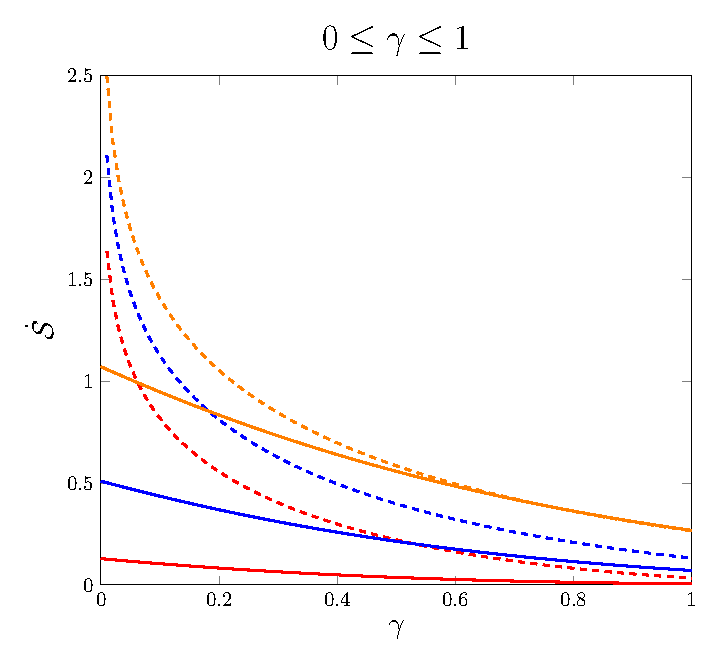
\includegraphics[width=0.32\textwidth]{figures/waiting_room_ent1.pdf}
%
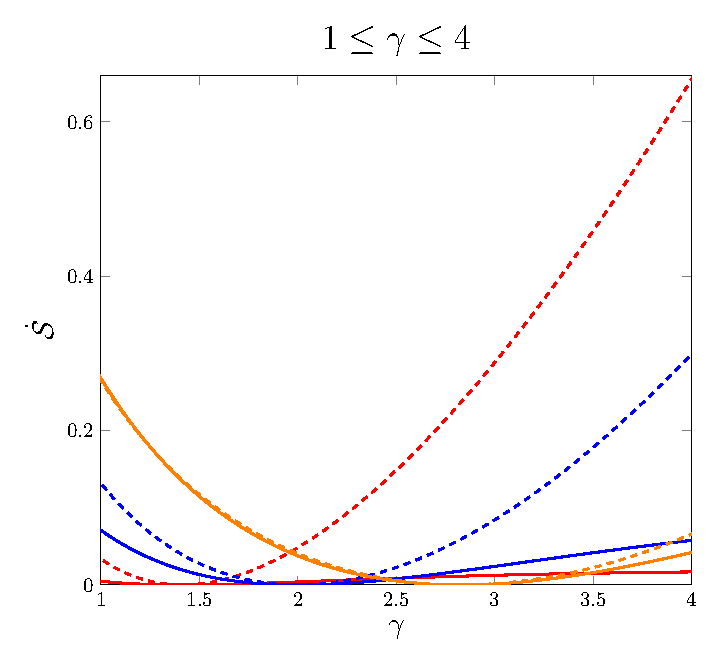
\includegraphics[width=0.32\textwidth]{figures/waiting_room_ent2.pdf}
%
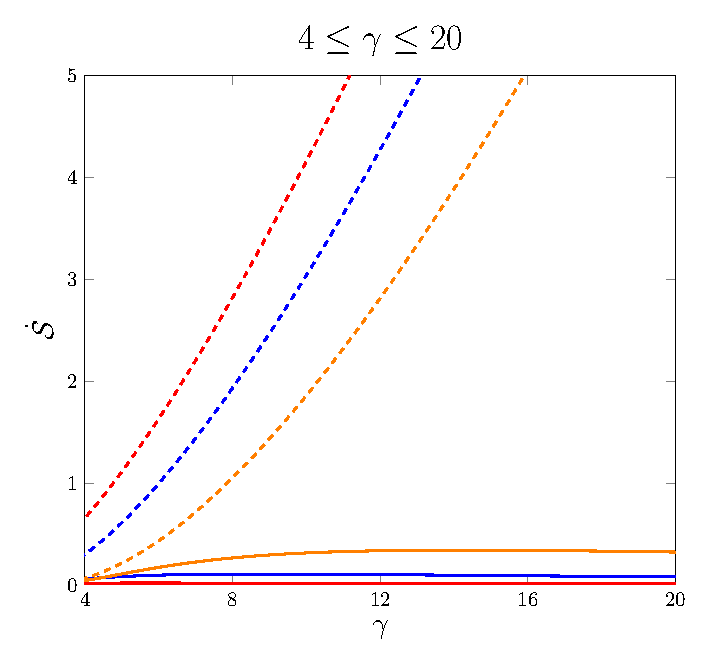
\includegraphics[width=0.32\textwidth]{figures/waiting_room_ent3.pdf}
%
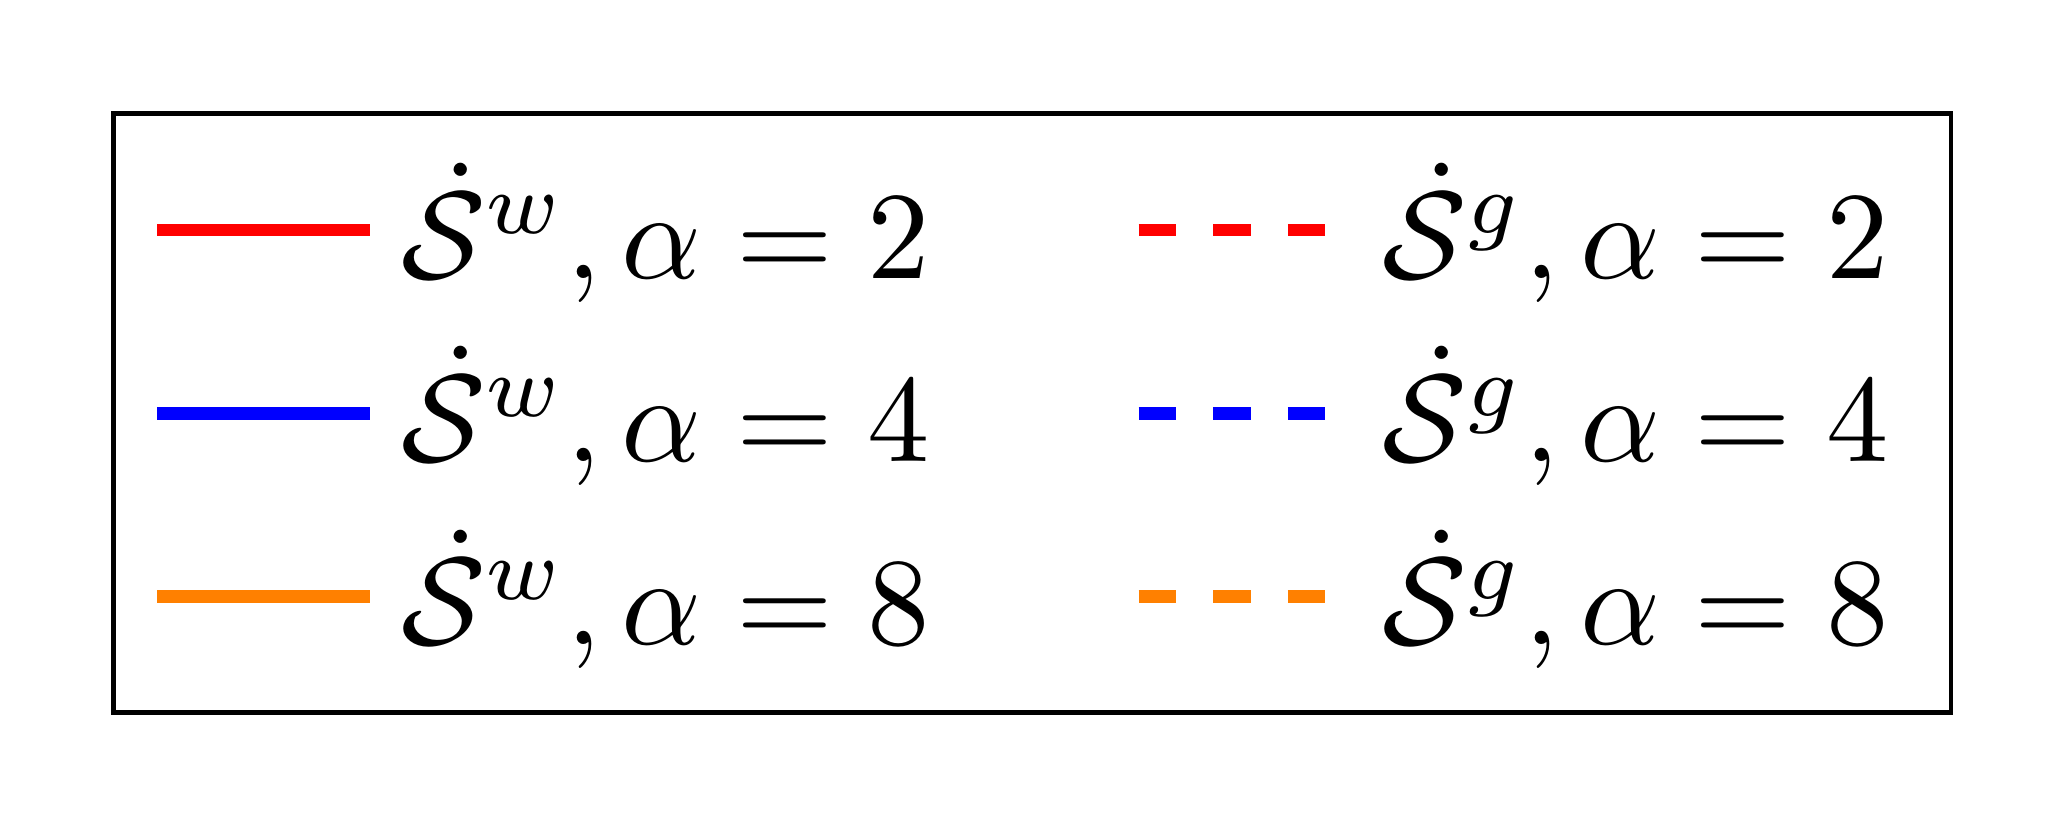
\includegraphics[width = 0.25\textwidth]{figures/waiting_room_entLegend.png}
\caption{\footnotesize Plots of $\entpp^w$ and $\entpp^g$ against $\gamma$ for different values of $\alpha$. Here we have set $\beta$ to unity and expressed $\gamma$ and $\alpha$ in multiples of $\beta$. Notice the different vertical scales. There is a zero of entropy production at $\gamma = \sqrt{\alpha}$ for both systems. $\entpp^w$ and $\entpp^g$ display qualitatively different behaviours in the limits as $\gamma \rightarrow 0$ and $\gamma \rightarrow \infty$.}
\label{fig:CG_waiting_room_entropy_prod}
\end{figure}

\subsubsection{Mechanism of Entropy Production}\label{subsection:mechanism-wating-room}

The dynamic entropy production of a continuous-time semi-Markov chain along non-equilibrium trajectories, $\entpp$ can be split into two contributions \cite{martinez2019inferring}

\begin{align}\label{entropy-split}
\entpp = \entpp_{\text{aff}} + \entpp_{\text{wtd}}.
\end{align}

$\entpp_{\text{aff}}$ results from what are called the cycle affinities of the system. If $\Gamma$ is the incidence graph of a semi-Markov chain, and $\mathcal{C}$ is a closed loop on $\Gamma$, then we define the cycle affinity, $\mathcal{A}_{\mathcal{C}}$, as

\begin{align}\label{cycle-affinity}
\mathcal{A}_{\mathcal{C}} = \log \prod_{(i\rightarrow j) \in \mathcal{C}} \frac{a_{ij}}{a_{ji}},
\end{align}

where $a_{ij}$ is the transition rate for $i \rightarrow j$ and we are are using the convention that $\log(\frac{0}{0}) = 0$. By dynamic reversibility, $a_{ij} > 0$ implies $a_{ji} > 0$, so $\mathcal{A}_{\mathcal{C}}$ is well-defined. Letting $r_{\mathcal{C}}$ be the rate at which the cycle $\mathcal{C}$ is observed in the long-time limit, we have \cite{van2022thermodynamic}

\begin{equation}
\entpp_{\text{aff}} = \sum_{\mathcal{C}} r_{\mathcal{C}}\mathcal{A}_{\mathcal{C}}
\end{equation}

$\entpp_{\text{wtd}}$ arises from asymmetric waiting-time distributions in semi-Markov systems. These waiting-time distributions carry information about the history of the system. For example, as the WR system transitions from $\ket{3}$ to $\ket{w}$, it enters the combination state

\begin{align}
\ket{w_3} = \frac{\beta}{\beta+\gamma}\ket{4} + \frac{\gamma}{\beta + \gamma}\ket{2},
\end{align}

which is distinct from the state $\ket{w_1}$ defined in (\ref{w1_comb_state}). The states $\ket{w_1}$ and $\ket{w_3}$ have different waiting-time distributions according to their time evolutions,

\begin{align}\label{w-evolutions}
\begin{split}
\ket{w_1(t)} &= \frac{1}{\alpha e^{-(\alpha + \gamma)t}+ \gamma e^{-(\beta + \gamma)t}}\left (\alpha e^{-(\alpha + \gamma)t}\ket{2} + \gamma e^{-(\beta + \gamma)t}\ket{4}\right) \\
\ket{w_3(t)} &= \frac{1}{\beta e^{-(\beta + \gamma)t} + \gamma e^{-(\alpha +\gamma)t}}\left (\gamma e^{-(\alpha + \gamma)t}\ket{2} + \beta e^{-(\beta + \gamma)}\ket{4} \right)
\end{split}
\end{align}

An observer viewing the process in reverse will observe state $\ket{w_3}$ when $\ket{w_1}$ occurs in the forward process. The distinct waiting-time distributions then give rise to entropy production which is captured in Eqns. (\ref{1to3_EP}) \& (\ref{3to1_EP}). In fact, $\entpp_{\text{wtd}}$ is the only contribution to the entropy production of the WR process. Cycles such as $\mathcal{C}_1 = \ket{1} \rightarrow \ket{w} \rightarrow \ket{1}$, which do not navigate the whole phase space, will not contribute to entropy production because they have zero cycle affinity. We have rates $\alpha + \gamma$ for the transition $\ket{1} \rightarrow \ket{w}$ and $\beta + \gamma$ for the transition $\ket{w} \rightarrow \ket{1}$, hence,

\begin{align}
\mathcal{A}_{\mathcal{C}_1} = \log \left( \frac{\alpha + \gamma}{\beta + \gamma}\frac{\beta + \gamma}{\alpha + \gamma}\right) = 0.
\end{align}

and likewise for any other cycle that does not explore the entire phase space. A similar calculation will show that in fact \textit{all} cycles of the WR system have zero affinity. The underlying physical intuition is that if a cycle includes an edge $(i \rightarrow j)$ then it necessarily includes the reversed edge $(j \rightarrow i)$. Hence, the forward and reverse trajectories include the same transitions, albeit in a different order. For the granular waiting room the situation is reversed.

Consider a clock-wise cycle of the granular system shown in Figure \ref{granular_fig}, beginning from $\ket{1}$ and making transitions
\begin{align}
\ket{1}\xrightarrow{} \ket{2}\xrightarrow{t_2} \ket{3}\xrightarrow{t_3} \ket{4}\xrightarrow{t_4} \ket{1},
\end{align}

where $t_i$ is the time spent occupying a state before transitioning away from it. The transition $\ket{1} \rightarrow \ket{2}$ occurs at $t=0$ and $\ket{4} \rightarrow \ket{1}$ at the final observation time $t = T$. In reverse time, the observed sequence of states is,

\begin{align}
\ket{1}\rightarrow\ket{4}\xrightarrow[]{t_4}\ket{3}\xrightarrow{t_3}\ket{2}\xrightarrow{t_2}\ket{1}.
\end{align}

In reverse time, the observed sequence of transitions is different, but the time interval spent in each state remains unchanged. Moreover, the waiting-time distribution for each state is independent of the particle's history. For these reasons, we have

\begin{align}
\entpp^g_{\text{wtd}} = 0
\end{align}

in the granular system. In summary, we have 

\begin{align}\label{ent-prod-mech}
\entpp^g = \entpp^g_{\text{aff}}, \; \; \entpp^w = \entpp^w_{\text{wtd}}.
\end{align}

We have already discussed how the quantitative behaviour of $\entpp^w$ is different from that of $\entpp^g$ as $\gamma$ is varied. Equation (\ref{ent-prod-mech}) shows that the two arise from completely separate mechanisms. Hence, coarse graining affects not only the degree of entropy production, but also its mechanism. 





% Since the Markov description of the granular waiting room is stable under time reversal, the waiting time in any state

\section{Unrequited Love}\label{chapter:UL1}

\textit{\textbf{Note}: for this section only, we shall use the convention $W = W_{ij} = W_{i \leftarrow j}$ for the transition matrices, such that the stationary probability vector $P_{\infty}$ is now a right eigenvector of $e^{tW}$. In this convention we have $\bra{j}M\ket{i} = M_{ij}$.}

\textit{In this section we derive an expression for the path probabilities of the elusive unrequited love system. We then anticipate an extension of the generating function approach to evaluating these probabilities in closed form.}
\subsection{System Description}

We couple a second Poisson process to a symmetric telegraph process described in Section \ref{chapter:telegraph}. A first particle, call it the leader, jumps independently between states $\ket{1}$ and $\ket{2}$. A second particle, call it the follower, shares this phase space, but it is coupled to the first particle. That is, the probability of a transition $\ket{i} \rightarrow \ket{j}$ for the follower depends on the state of the leader. The phase space of the two particle system is $\mathcal{X} = \{ \ket{11}, \ket{12}, \ket{22}, \ket{21}\}$ where $\ket{x_Ax_B} = \ket{11}$ is the state where both particles are in state $\ket{1}$ of their marginal system and so on. $\ket{x_A}, \ket{x_B}$ denotes the state of the leader and the follower, respectively. The two particle ensemble we shall call the granular Unrequited Love (UL) system. The time evolution of the granular UL system is governed by the master equation

\begin{align}
\dot{P}(t) = e^{tW}P(t), \; \; \;  W = \begin{pmatrix} -\alpha - \beta & \alpha & \beta + \gamma & 0 \\
  \alpha & -\alpha -\beta -\gamma & 0 & \beta \\
  \beta & 0 & -\alpha-\beta-\gamma & \alpha \\
  0 & \beta+\gamma & \alpha & -\alpha-\beta\end{pmatrix}.
\end{align}

\begin{wrapfigure}{R}{0.45\textwidth}
\centering
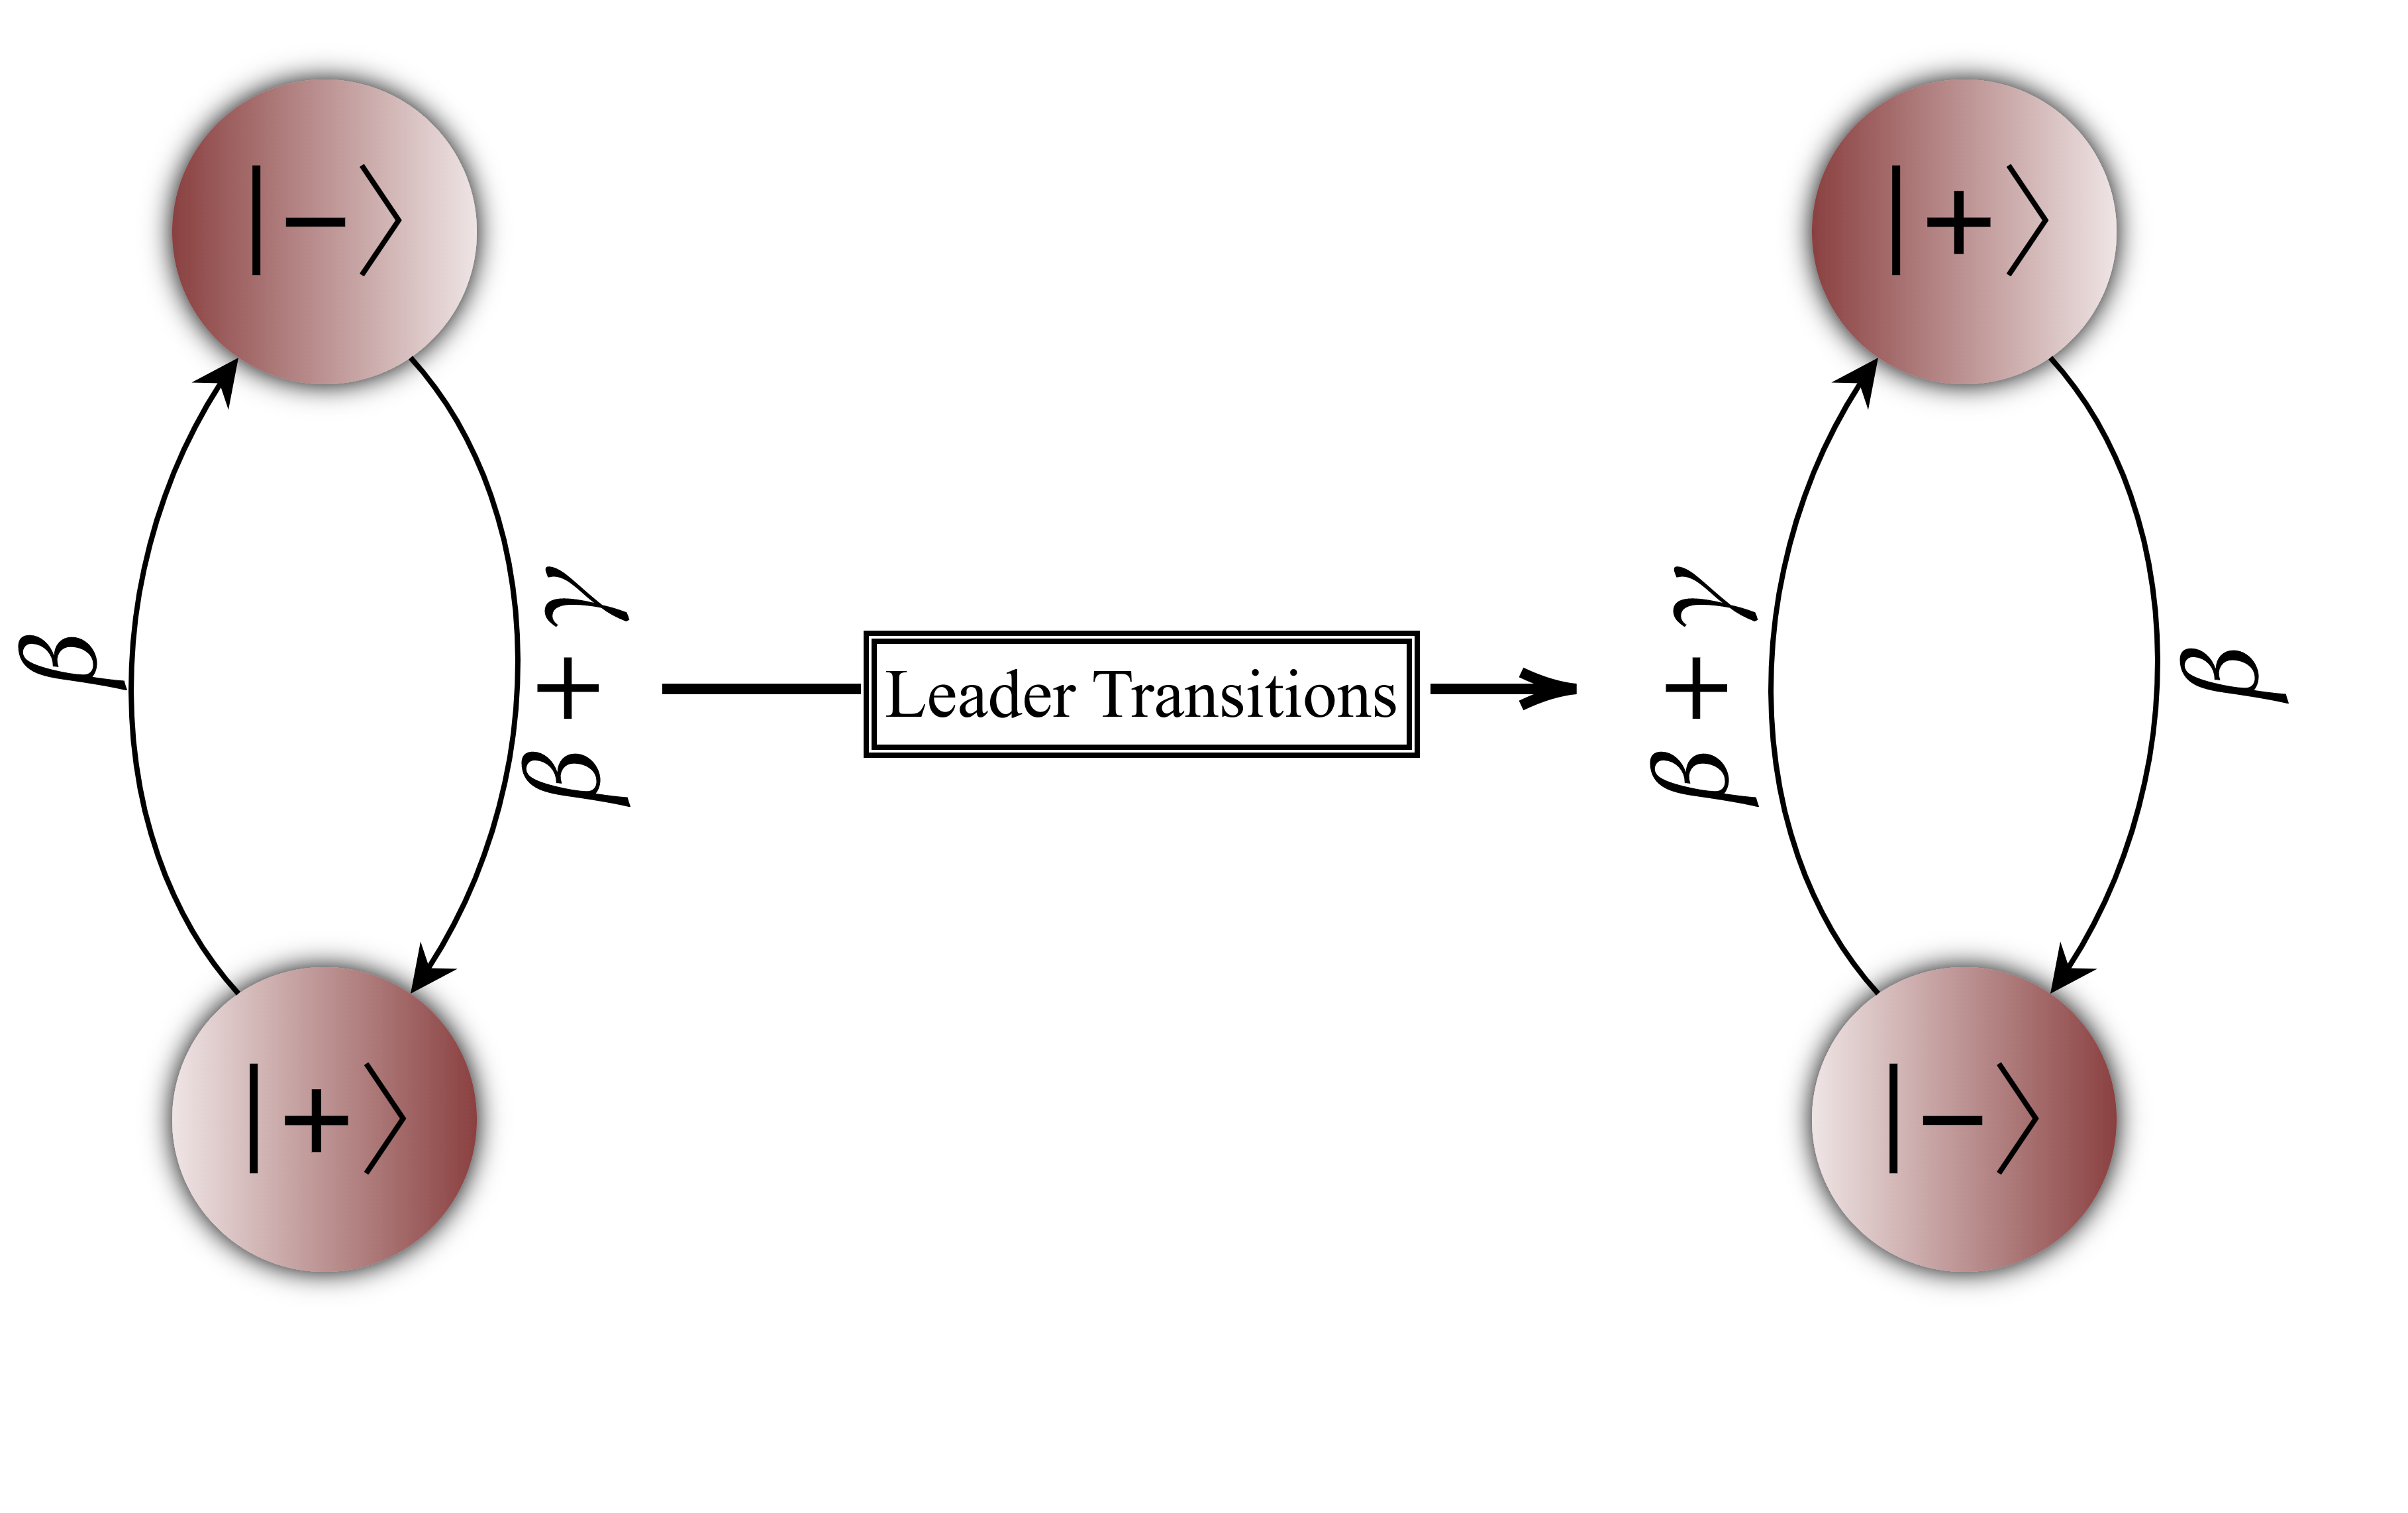
\includegraphics[width = 0.4\textwidth]{figures/follower_pov.png}
\caption{\footnotesize From the point of view of the follower particle, the states $\ket{1}$ and $\ket{2}$ are completely symmetric. The only asymmetry is brought about by the transitions of the leader which, in effect, switch the follower's preference for one state over the other. In this figure, the leader particle at first occupies the bottom state, meaning that the follower prefers it. Once the leader transition to the top state, the follower tends also to favour that state in its transitions. In this way, either of the state $\ket{1}$ or $\ket{2}$ can play the role of $\ket{+}$ as seen here.}
\label{follower-pov}
\end{wrapfigure}

With respect to the phase space, $W$ has the basis ordering $e_1 = \ket{11}$, $e_2 = \ket{21}$, $e_3 = \ket{12}$, and $e_4 = \ket{22}$, so that, for example, $W_{12}$ is the rate for the transition $\ket{21} \rightarrow \ket{11}$. As usual $\omega \in \Omega$ denotes a single path for the entire ensemble. We shall denote the leader's and follower's path by $\omega_A \in \Omega_A$ and $\omega_B \in \Omega_B$ respectively. Let $M = \mathds{1} + \tau W$ be the stochastic matrix of the discretised process. We intend to take the limit $\tau \rightarrow \rmd t$. Let us also write $M$ in block form 

\begin{align}
M = \begin{pmatrix} M_1 & M_2 \\ 
M_3 & M_4\end{pmatrix}.
\end{align}


The reason for this representation will become clear presently. We shall make the UL process non-Markov by hiding the leader's path from the observer, i.e. the observer shall only have access to $\omega_B$ and not to $\omega_A$. In this case, the observer cannot observe the states $\ket{11}$, $\ket{12}$, $\ket{21}$, and $\ket{22}$ individually. They may only observe convex combinations of the form $a\ket{11} + b\ket{21}$ and $a\ket{22} + b\ket{12}$. This coarse-grained system we will call the Unrequited Love (UL) process. When the observer measures $x_B = \ket{1}$ at time $t=0$, we deduce that the UL system is in the combination state $1/2 \ket{11} + 1/2 \ket{21}$. The normalisation factor is $1/2$ because the leader has no preference for either state. But note that this state can evolve non-trivially with time depending on the observed path $\omega_B$. The longer the follower is observed to stay in $\ket{1}$, the more likely it is that the underlying state of the granular UL system is $\ket{11}$, since, in a small time interval, the follower is less likely to transition away from $\ket{11}$ than from $\ket{21}$.\footnote{See the evolution equation for the states $\ket{w_1(t)}, \ket{w_3(t)}$ in Eqn. (\ref{w-evolutions})}

\begin{figure}
  \begin{subfigure}[b]{0.49\textwidth}
  \centering
  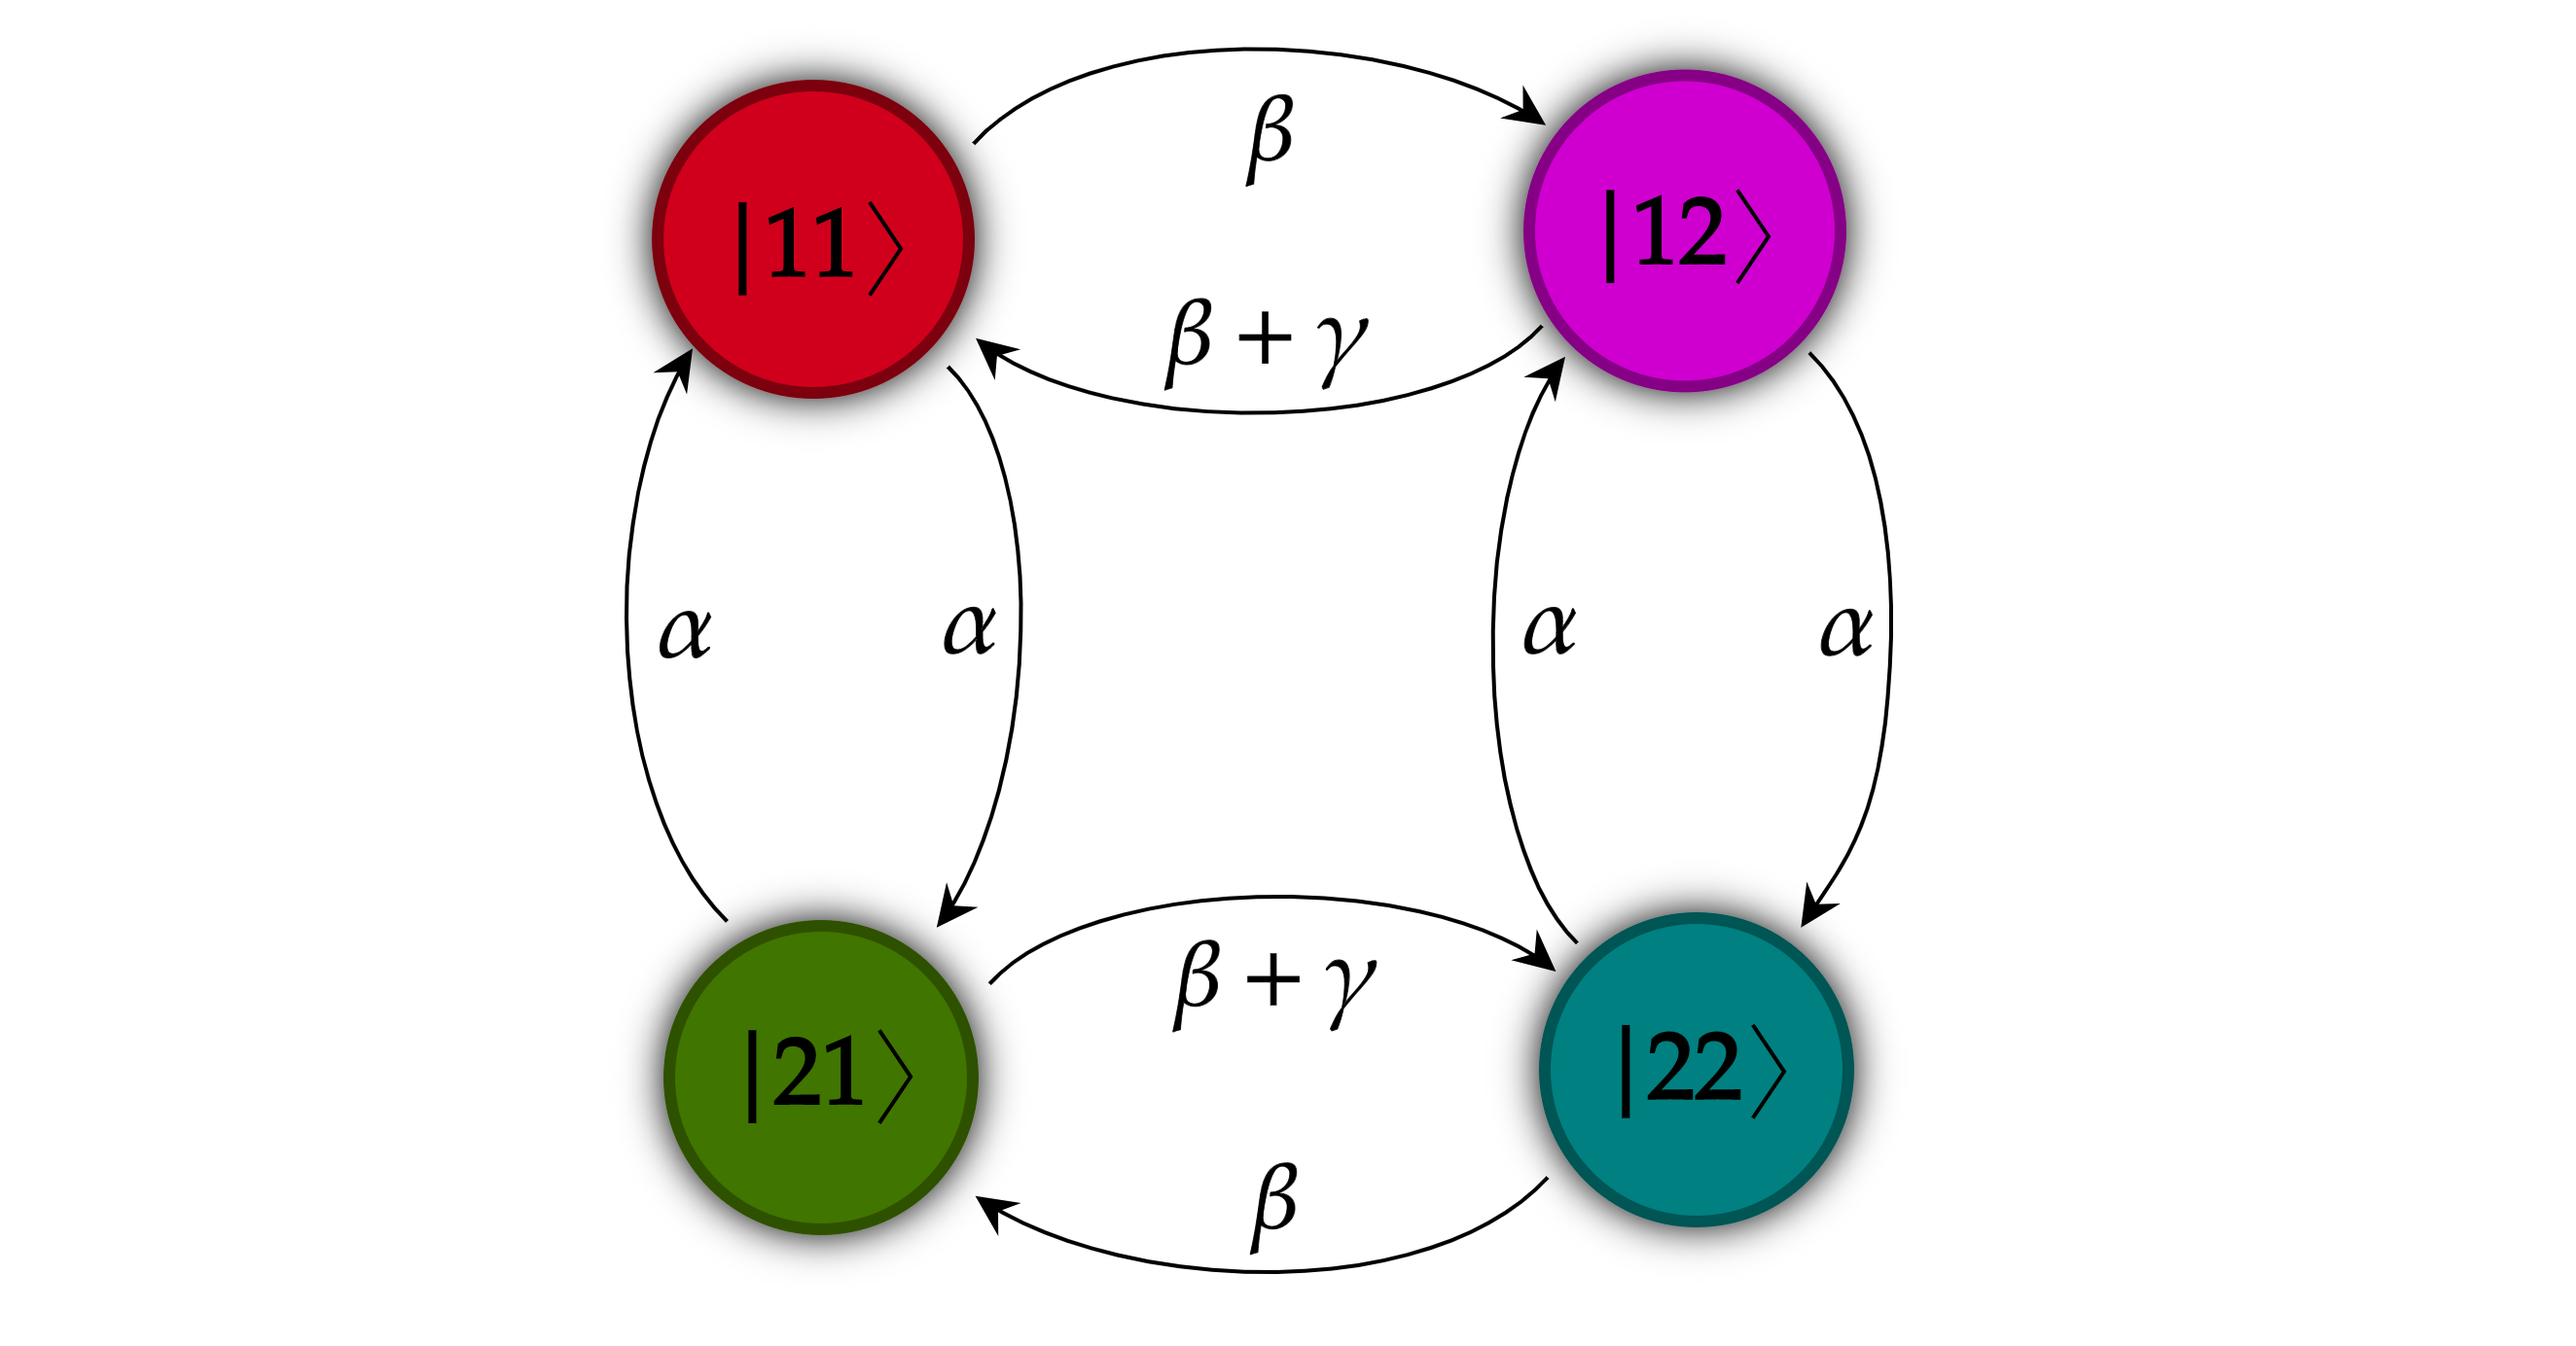
\includegraphics[width = \textwidth]{figures/UL_granular.png}
  \caption{Granular UL process}
  \label{granular_UL}
\end{subfigure}
\begin{subfigure}[b]{0.49\textwidth}
  \centering
  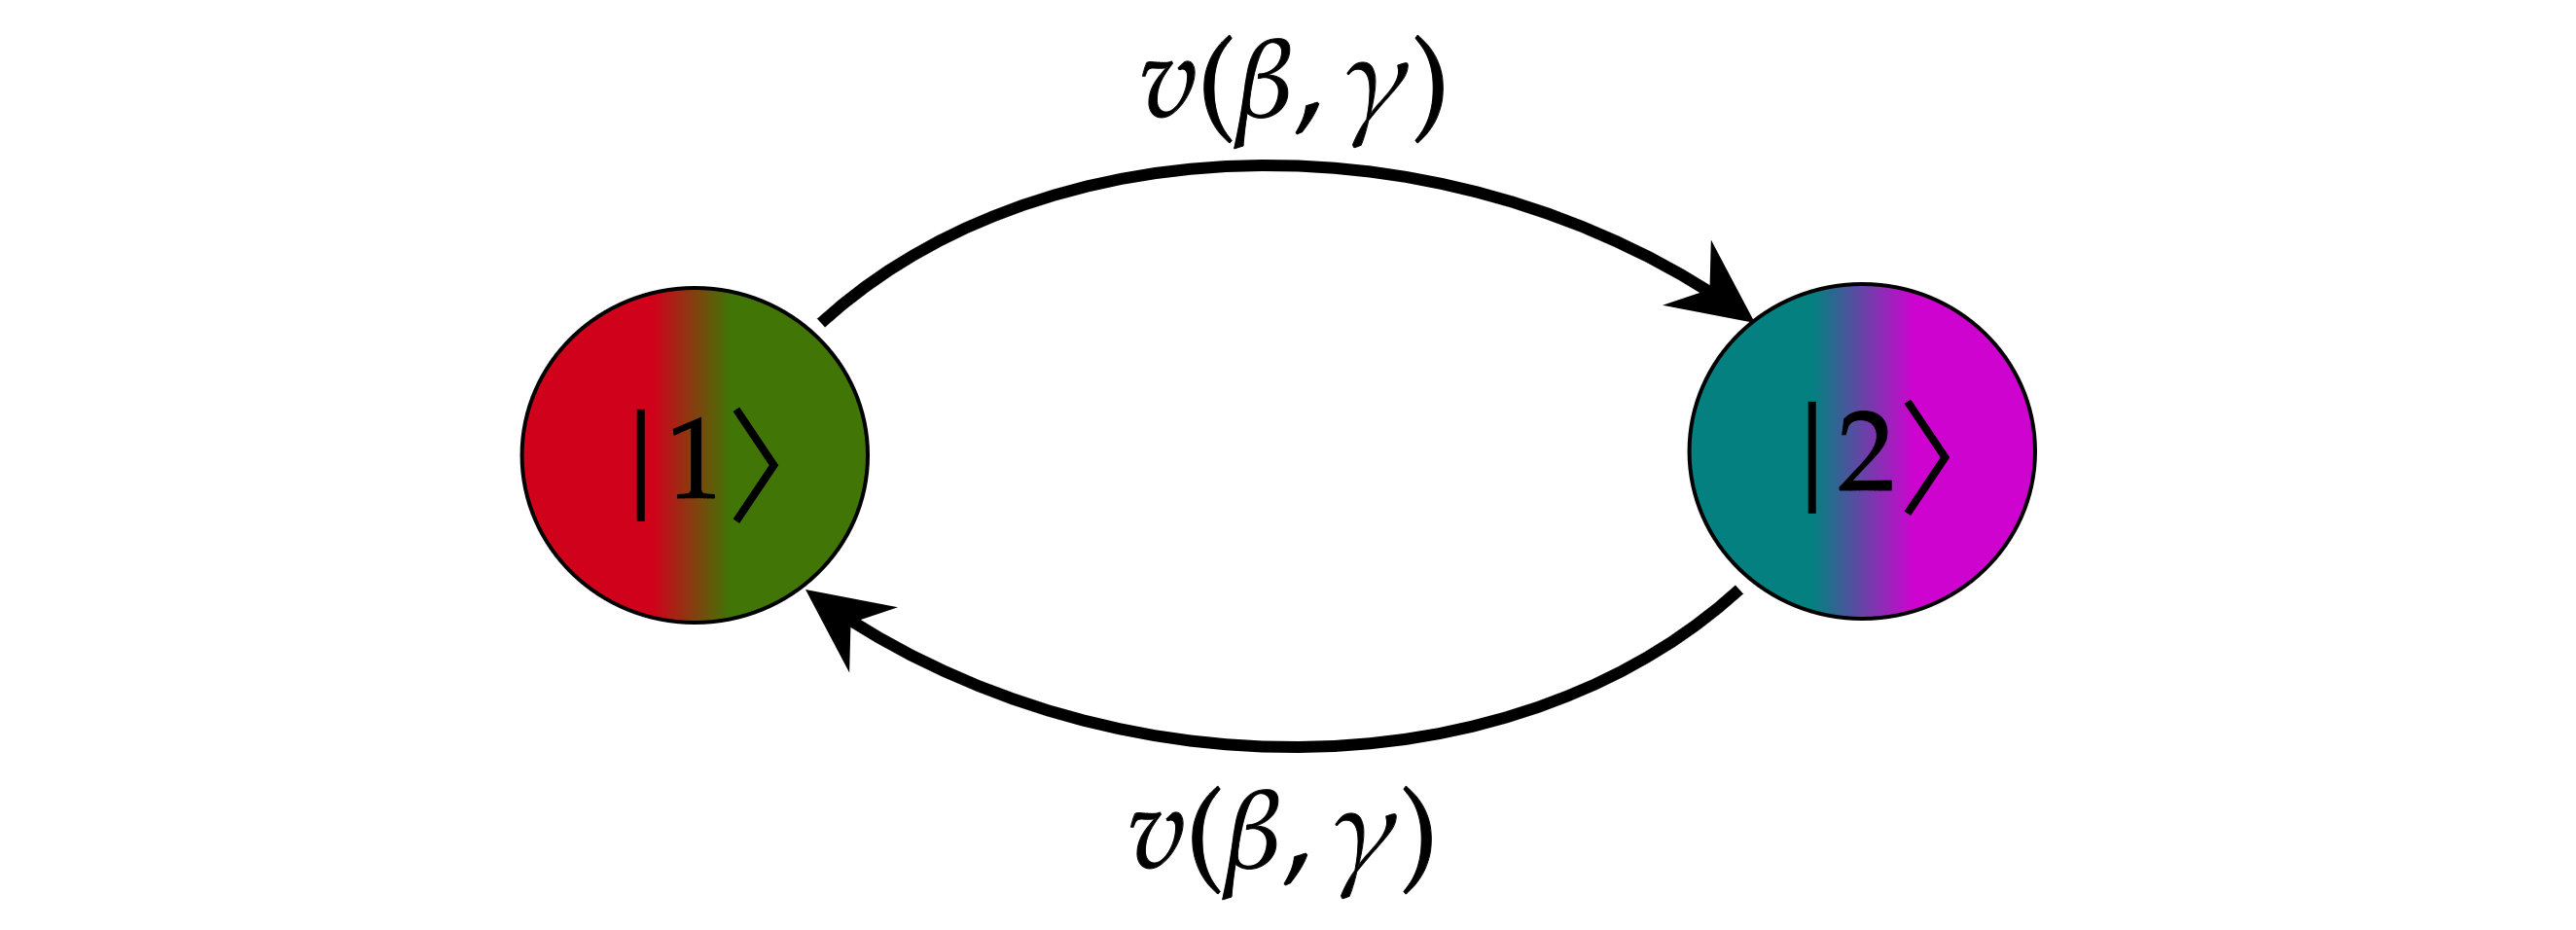
\includegraphics[width = \textwidth]{figures/UL.png}
  \caption{UL process}
  \label{coarse_grained_UL}
\end{subfigure}
\caption{\footnotesize Subfigure \ref{granular_UL} shows the layout of the granular UL system. The granular UL is a four-state continuous-time Markov chain. \ref{coarse_grained_UL} shows the states of the granular UL system collapsed together to give the UL process. In this picture, the follower hops between states $\ket{1}$ and $\ket{2}$ with some effective rate $v(\beta,\gamma)$. If one observes the UL system throughout the interval $[0,T]$, then the rate $v = v(t, \beta, \gamma)$ will be a process driven by the leader. See also Figure \ref{follower-pov}}
\label{system_desc_fig_UL}
\end{figure}


\subsection{Path Probability Derivation}

The probability of a path $(\omega_A, \omega_B)$ is 

\begin{align}
\bP(\omega_A, \omega_B) = \bra{x^1_Ax^1_B}M\ket{x^2_Ax^2_B}\ldots M\ket{x^N_Ax^N_B},
\end{align}

where $x^i_j$ is the state of particle $j$ at the $i$-th time step. Our aim is to derive the marginal probability of $\omega_B$ 

\begin{align}
\bP(\omega_B) = \sum_{\omega_A \in \Omega_A} \bP(\omega_A,\omega_B).
\end{align}

This will be  the probability accessible to the observer, since $\omega_A$ is hidden from them. We will perform this sum by summing over the possible trajectories of the leader at each step. For example, if $N=3$ and $\omega_B = \{\ket{1},\ket{1} , \ket{1}\} $, then

\begin{align}\label{path-prob-example}
\begin{split}
\bP(\omega_B) &= \frac{1}{2}\left (\bra{11} + \bra{21}) \right)M\left(\ket{11}\bra{11} + \ket{21}\bra{21}\right)M\left (\ket{11} + \ket{21} \right)\\
&= \frac{1}{2} \left (\bra{11} + \bra{21}\right) \begin{pmatrix}M_1 & 0 \\ 
M_3 & 0\end{pmatrix}M\left (\ket{11} + \bra{21} \right)\\ 
&= 1-2(\beta + \gamma/2)\tau + \mathcal{O}(\tau^2),
\end{split}
\end{align}

where we have used the fact that

\begin{align}
\ket{11}\bra{11} = \begin{pmatrix} 1 & & & \\ 
& 0 & & \\ 
& & 0 & \\ 
& & & 0\end{pmatrix}, \; \; \; \ket{21}\bra{21} = \begin{pmatrix} 0 & & & \\ 
& 1 & & \\ 
& & 0 & \\ 
& & & 0\end{pmatrix}.
\end{align}

The matrix blocks $M_1$ and $M_2$ contain all the information about transitions away from the states $\ket{11}$, $\ket{21}$, hence they appear when the CGUL system is in a combination of these states. Likewise, $M_2$ and $M_4$ will appear in the sum whenever the path indicates that the CGUL occupies $a\ket{22} + b\ket{12}$. Note also that the parameter $\alpha$ does not appear on the LHS of Eqn (\ref{path-prob-example}) since the nuisance paths of the leader have been summed over. 

Suppose now that the path $\omega_B$, composed of $t/\tau = N = \sum m_i$ total steps, is such that the follower spends $m_1$ steps in $\ket{1}$, $m_2$ steps in $\ket{2}$, then again  $m_3$ steps in $\ket{1}$ and so on until the path ends with the follower in $\ket{1}$ for $m_{L+1}$ steps (such that there are a total of $L$ transitions for the follower). Then we can write the path probability of $\omega_B$ as

\begin{align}
\bP(\omega_B) &= \frac{1}{2}\left(\bra{11} + \bra{21} \right)\begin{pmatrix} M_1 & 0 \\ M_3 & 0 \end{pmatrix}^{m_1-1}\begin{pmatrix} 0 & M_2 \\ 0 & M_4 \end{pmatrix}^{m_2}\ldots\begin{pmatrix} M_1 & 0 \\ M_3 & 0 \end{pmatrix}^{m_{L+1}-1}M\left (\ket{11} + \ket{21} \right) \\ 
\label{before-sum}
&= \frac{1}{2}\begin{pmatrix} 1 & 1 & 0 & 0\end{pmatrix}\begin{pmatrix} M_1 & 0 \\ M_3 & 0 \end{pmatrix}^{m_1-1}\begin{pmatrix} 0 & M_2 \\ 0 & M_4 \end{pmatrix}^{m_2}\ldots\begin{pmatrix} M_1 & 0 \\ M_3 & 0 \end{pmatrix}^{m_{L+1}-2}M \begin{pmatrix} 1 \\ 1 \\ 0 \\ 0 \end{pmatrix} \\ 
\label{after-sum}
&= \begin{pmatrix}1 & 1 \end{pmatrix} M_1^{m_1-1}M_2M_4^{m_2-1}M_3M_1^{m_3-1}\ldots M_3M_1^{m_{L+1}-1}\begin{pmatrix} 1 \\ 1\end{pmatrix} \\\label{path-density} &\eqqcolon \begin{pmatrix}1 & 1 \end{pmatrix}\phi\begin{pmatrix} 1 \\ 1\end{pmatrix}.
\end{align}

In Appendix \ref{appendix:recovering} we show how (\ref{after-sum}) follows from (\ref{before-sum}). If $t_i$ is the time of the $i$-th transition, we shall define $\tilde{t}_i = t_i - t_{i-1}$ such that $\sum_i \tilde{t}_i = t$. Here we use the convention $t_0 = 0$ and $t_{L+1} = t$. The $\tilde{t}_i$'s are the times spent in a state before transitioning. The limit $\tau \rightarrow \rmd t$ is equivalent to $N \rightarrow \infty$. Taking this limit while keeping the ratios $m_i/N$ fixed, for $j = 1,4$ we have 

\begin{align}
\lim_{N\rightarrow \infty} M_j^{m_i} =  \lim_{N\rightarrow \infty} ( 1+ \frac{t}{N}W_j)^{Nm_i/N} = e^{\tilde{t}_iW_j},
\end{align}

where $W_j$ is the $j$-th block of the matrix $W$ and $ \sum t_i = t$. On the other hand, for $j=2,3$, and in the limit of large $N$, we have $M_j \rightarrow W_j \rmd t $. For the rest of this section, we will abuse the notation to denote $\tilde{t}_i$ by $t_i$. So, in the large $N$ limit we have\footnote{See the derivation of the path probability in Section \ref{chapter:telegraph}}

\begin{align}
M_1^{m_i}M_2 \rightarrow \rmd t_i e^{t_iW_1}W_2, \; \; \; M_4^{m_i}M_3 \rightarrow \rmd t_i e^{t_iW_4}W_3.
\end{align}

Hence we have the limit 

\begin{align}\label{phi-limit}
\lim_{N\rightarrow \infty} \phi = \rmd t_1 \ldots \rmd t_L e^{t_1W_1}W_2e^{t_2W_4}W_3\ldots W_3e^{t_{L+1}W_1}.
\end{align}

In the sequel we will suppress the infinitesimals $\rmd t_1 \ldots \rmd t_L$ for brevity. Evaluating this product of matrices will give the density of paths that make $L$ transitions in time $t$. In general finding a closed form for (\ref{phi-limit}) is not trivial. We outline here our most promising approach. 

We will assume that $\gamma^2/\alpha^2, \gamma^2/\beta^2 \ll 1$ and we will ignore contribution of these orders. We first note the commutation relation

\begin{align}
\begin{split}
  e^{t_i W_4}W_3 &= W_3e^{t_i W_4} + \left[e^{t_i W_4}, W_3\right]  \\
  &=  W_3e^{t_i W_4} + (\alpha\gamma)\frac{2\sinh\left(\frac{t_i}{2}\sqrt{4\alpha^2+\gamma^2}\right)}{\sqrt{4\alpha^2+\gamma^2}} \begin{pmatrix} 0 && 1 \\ -1 && 0 \end{pmatrix}  \\
  &=  W_3e^{t_i W_4} + \gamma\sinh(\alpha t_i)  \begin{pmatrix} 0 && 1 \\ -1 && 0 \end{pmatrix} + \mathcal{O}(\gamma^2/\alpha^2).
 \end{split}
\end{align} 

Using this, and the fact that $W_2W_3 = \beta(\beta +\gamma)\mathds{1}$, we rewrite (\ref{phi-limit}) as 

\begin{align}\label{limit-phi-prod}
\begin{split}
\lim_{N\rightarrow \infty}\phi &= \left(\prod_{i=1}^{L/2}\left(e^{t_{2i-1} W_1} W_2 W_3
    e^{t_{2i} W_4} + \gamma\sinh(at_{2i}) e^{t_{2i-1} W_1} W_2\begin{pmatrix} 0 && 1 \\ -1 && 0 \end{pmatrix} \right)\right)e^{t_{L+1} W_1} \\
    &=  \left(\prod_{i=1}^{L/2}\left(\beta(\beta+\gamma)e^{t_{2i-1} W_1}e^{t_{2i} W_4} + \gamma(\beta+\gamma) \sinh(\alpha t_{2i})e^{t_{2i-1} W_1}\begin{pmatrix} 0 && 1 \\ -\beta/(\beta+\gamma) && 0 \end{pmatrix} \right)\right)e^{t_{L+1} W_1}.
\end{split}
\end{align}

By the binomial theorem, it follows that
\begin{align}
\lim_{N\rightarrow \infty}\phi = \left(\sum_{k=0}^{L/2} \beta^{L/2}(\beta +\gamma)^{L/2}\left(\frac{\gamma}{\beta}\right)^k\tilde{\phi}_k\right) e^{t_{L+1} W_1}
\end{align}

for appropriate matrices $\tilde{\phi}_k$. Each term in the above has a  coefficient proportional to $\gamma^k/\beta^k$ for some $k = 0, 1,\ldots L/2 $. Ignoring terms that have $k \geq 2$, we arrive at 

\begin{align} 
\lim_{N\rightarrow \infty}\phi = \phi_0 + \phi_1 + \mathcal{O}(\gamma^2/\beta^2),
\end{align}

where $\phi_0$ is the leading order term and $\phi_1$ is the sum of first order terms in $\gamma/\beta$. In Appendix \ref{appendix:recovering} we show that the contribution of $\phi_1$ to the path density (\ref{path-density}) is in fact $\mathcal{O}(\gamma^2/\beta^2, \gamma^2/\alpha\beta)$. It remains to evaluate

\begin{align}
\phi_0 = \rmd t_1 \ldots \rmd t_L \beta^{L/2}(\beta + \gamma)^{L/2}e^{t_1 W_1}e^{t_2 W_4}e^{t_3 W_1}\ldots e^{t_L W_4}e^{t_{L+1} W_1}.
\end{align}

Consider the basis of $\mathfrak{sl}(2)$ given by 

\begin{equation}
  H = \begin{pmatrix}1 && 0 \\ 0 && -1 \end{pmatrix}, \; \; X_+ = \begin{pmatrix}0 && 1 \\ 1 && 0 \end{pmatrix}, \;\; X_- = \begin{pmatrix}0 && -1 \\ 1 && 0 \end{pmatrix},
\end{equation}

and define the two families of indexed operators given by 

\begin{align}
  a_m = \left(\frac{m\gamma}{2\alpha}H + X_+ \right), \; \;
  b_m = \left(\mathds{1} + \frac{m\gamma}{2\alpha}X_-\right), \; \; m\in \bZ.
\end{align}

Notice that $a_m$ and $b_m$ are traceless for all $m$. Using this definition, we can write $W_1 = a_1 - (\alpha + \beta + \gamma/2) \mathds{1}$ and $W_4 = a_{-1} - (\alpha + \beta + \gamma/2)\mathds{1}$. Hence, by Proposition \ref{mat-exp-lemma}, `

\begin{align}\label{W1-exponential}
e^{t_iW_1} &= e^{-(\alpha +\beta+\gamma/2)t_i}\left(\cosh(\alpha t_i)\mathds{1} + \sinh(\alpha t_i) a_1 \right) + \mathcal{O}(\gamma^2/\alpha^2) \\
\label{W4-exponential}
e^{t_iW_4} &= e^{-(\alpha +\beta+\gamma/2)t_i}\left(\cosh(\alpha t_i)\mathds{1} + \sinh(\alpha t_i) a_{-1} \right) + \mathcal{O}(\gamma^2/\alpha^2).
\end{align}

Moreover, up to $\mathcal{O}(\gamma^2/\alpha^2)$, the following operator algebra holds\footnote{This means that, e.g., $a_ma_n = b_{n-m} + \mathcal{O}(\gamma^2/\alpha^2)$.}

\begin{align} 
a_ma_n &= b_{n-m} \\
  a_mb_n &= a_{m+n} \\
  b_na_m &= a_{m-n} \\
  b_nb_m &= b_{m+n}.
\end{align}

Using this algebra, any sequence of operators $a_{i_1}\ldots a_{i_N}$ where $i_n = 1, -1,$ is equal either to $b_m$ or $b_ma_1$ for some $m \in \bZ$. For example
\begin{align}
a_1a_{-1}a_{1} = (a_1a_{-1})a_{1} = b_{-2}a_{1}.
\end{align}

Note also that $a_ma_m = b_0 = \mathds{1}$, hence

\begin{align}
\begin{split}
b_ma_{\pm 1} &= b_ma_{\pm 1}a_{\mp 1}a_{\mp 1} \\
&= b_mb_{\mp 2} a_{\mp 1}\\
&= b_{m \mp 2}a_{\mp 1}.
\end{split}
\end{align}

Using (\ref{W1-exponential}) and (\ref{W4-exponential}) we can write for $\phi_0$

\begin{align}\label{phi0_factorised}
\begin{split}
\phi_0 &= \rmd t_1 \ldots \rmd t_L \beta^{L/2}(\beta + \gamma)^{L/2} e^{-(\alpha + \beta +\gamma/2)t}\bigg(\cosh(\alpha t_1)\mathds{1} + \sinh(\alpha t_1) a_1 \bigg)\bigg(\cosh(\alpha t_2)\mathds{1} + \sinh(\alpha t_2) a_{-1} \bigg)\\
&\quad \quad \ldots\bigg(\cosh(\alpha t_{L+1})\mathds{1} + \sinh(\alpha t_{L+1}) a_1 \bigg) \\ 
&= \rmd t_1 \ldots \rmd t_L \beta^{L/2}(\beta + \gamma)^{L/2}e^{-(\alpha + \beta +\gamma/2)t}\left (\prod_i \cosh(\alpha t_i) \right)\bigg( \mathds{1} + \tanh(\alpha t_1) a_1\bigg)\bigg( \mathds{1} + \tanh(\alpha t_2) a_{-1}\bigg)\\ &\quad \quad \quad \quad \ldots\bigg(\mathds{1} + \tanh(\alpha t_{L+1})a_1\bigg)  
\end{split}
\end{align}

If the leader has a very slow transition rate, then the distribution of time between two transitions of the follower approaches a double exponential distribution. When $\alpha$ is comparable to $\beta$, the underlying waiting-time distribution for the follower alternates depending on the state of the leader. The appearance of hyperbolic functions in $\alpha t_i$ indicates an averaging of these double exponential distributions. Indeed, when $\alpha \ll \beta$, we expect that $\alpha t_i \ll 1$ hence $\tanh (\alpha t_i) \approx 0$, and we are left with a double exponential distribution for each transition. It is doubtful, however, if considering the case $\alpha \ll \beta$ systematically will be of much physical relevance. Since we have already assumed $\gamma \ll \alpha, \beta$, imposing this new condition would constrain the analysis to those cases where $\gamma \ll \alpha \ll \beta$.

It is difficult to progress much further with the evaluation of $\phi_0$ into closed form. The chief difficulty is that, since the waiting times of the follower contain information about the position of the leader, the $t_i$ are not independent random variables. However, understanding products of the form $e^{t_1A}e^{t_2B}\ldots e^{t_LA}$ is of some mathematical interest (see for example \cite{friedland1994product, cohen1982eigenvalue}). So, in the interest of extending the analysis, we will recast Eqn. (\ref{phi0_factorised}) into a form which resembles a generating function, allowing combinatorial techniques to be used in future work. Define  $w_i = \tanh(\alpha t_i)$. Then From Eqn. (\ref{phi0_factorised}), we surmise that 

\begin{align}\label{phi0-prop-to}\small
\phi_0 &\propto e^{-(\alpha + \beta +\gamma/2)t}\left (\prod_i \cosh(\alpha t_i) \right)\bigg( \mathds{1} + \tanh(\alpha t_1) a_1\bigg)\bigg( \mathds{1} + \tanh(\alpha t_2) a_{-1}\bigg)\nonumber\\ &\quad \quad \quad \quad\ldots\bigg(\mathds{1} + \tanh(\alpha t_{L+1})a_1\bigg) \\ 
&= e^{-(\alpha + \beta +\gamma/2)t}\left(\prod_i \frac{1}{\sqrt{1-w_i^2}} \right)\left(\sum_{m = -L/2}^{L/2}c^0_m(w_i)b_m + \sum_{m = -L/2}^{L/2}c^1_m(w_i)b_ma_1\right)
\end{align}

where we have used the identity 

\begin{align}
\tanh^2 x + \sech^2 x = 1.
\end{align}

Recall that the RHS of (\ref{phi0-prop-to}) was obtained by expanding the product $e^{t_1 W_1}e^{t_2 W_4}e^{t_3 W_1}\ldots e^{t_L W_4}e^{t_{L+1} W_1}$. The equality 

\begin{align}\label{generating-function}
\bigg( \mathds{1} + w_1 a_1\bigg)\bigg( \mathds{1} + w_2 a_{-1}\bigg)\ldots\bigg(\mathds{1} + w_{L+1}a_1\bigg) =\left(\sum_{m = -L/2}^{L/2}c^0_m(w_i)b_m + \sum_{m = -L/2}^{L/2}c^1_m(w_i)b_ma_1\right)\label{generating-function}
\end{align}


resembles a generating function, with the chief difference that the $a_{\pm1}$'s do not commute. In every case, $c_m^k(w_i)$ is a polynomial in the $w_i$'s such that $w_j$ can only appear once in each term of the polynomial for fixed $j$. Further simplifications can be made if one assumes that the $t_i$ (and hence the $w_i$) are i.i.d. random variables. 

\subsection{Discussion}
The above analysis of the UL process demonstrates how a path-space approach to coarse-grained processes is in general highly non-trivial. This appears to be especially true of what we shall later venture to call `Lego brick processes' (See Section \ref{chapter:classification}).
Generating functions are an established method in combinatorics. They are usually used to count the subsets of a certain description from a set of given size. It is hoped that the method of generating functions can be extended to count permutations (rather than simply subset) of a given description. A method of counting the permutations of the operators $a_1$ and $a_{-1}$ in the expansion of the LHS of Eqn. (\ref{generating-function}) would provide a path forward for evaluating the coefficients $c^k_m(w_i)$ in closed form. 

An important limitation of the derivation above is that we have kept $L$ fix throughout. In particular, we have not considered the case of large $L$. At several stages in the derivation, we ignore terms of order $\mathcal{O}(\gamma^2/\beta^2)$ or above without considering how these terms scale with $L$. Consider, for example, the expression 

\begin{align}
\lim_{N\rightarrow \infty}\phi = \left(\sum_{k=0}^{L/2} \beta^{L/2}(\beta +\gamma)^{L/2}\left(\frac{\gamma}{\beta}\right)^k\tilde{\phi}_k\right) e^{t_{L+1} W_1}.
\end{align}

We go on to ignore terms in the above that are $\mathcal{O}(\gamma^2/\beta^2)$ or smaller. This means ignoring $\tilde{\phi}_{k}$ for $k \geq 2$. If $L$ is small, then this will not present any problems. However, taking note of Eqn. (\ref{phi-limit}), as $L$ grows large, $\tilde{\phi}_k$ grows as 

\begin{align}
\tilde{\phi}_k \sim \binom{L/2}{k} \sim (L/2)^k, \quad L \gg k.
\end{align}

This is because there are $\binom{L/2}{k}$ terms of order $\mathcal{O}(\gamma^k/\beta^k)$ in the expansion for $\phi$. So, in general, a perturbative approach to the path probabilities of the UL process will need to treat the limits of small $\gamma$ and large $L$ concurrently. If we confine ourselves to small observation time $t$, then the total probability of making $L \gg 1$ jumps is small, so the analysis presented heretofore holds. \newpage
\section{Coarse-grained Diffusion Processes}\label{chapter:RnT}
\textit{ \textbf{Acknowledgment:} the work in this section was done in close collaboration with Jacob Knight and Gunnar Pruessner}

\textit{In this section we derive a novel pertubative approach to calculating the entropy production of coarse-grained diffusion process. We then apply this technique to find the leading order contribution to the entropy production rate of an asymmetric Run-and-Tumble particle.}
\subsection{System Description}
Let $w(t)$ be any stochastic process. Consider a self-propelled particle whose motion is governed the SDE 

\begin{align}\label{main-langevin}
    \rmd x_t = \nu w(t)\rmd t +\sqrt{2D}\rmd B_t, \quad x(0) = 0,
\end{align}

where $\nu$ is a dimensionless book-keeping parameter and $B_t$ is a Brownian motion independent of $w(t)$, i.e. a Gaussian process such that
\begin{align}\label{white-noise-prop}
\begin{split}
\bE B_t &= 0 \\ 
\bE B(t)B(s) &= \min(t,s).
\end{split}
\end{align}

In the sequel, Equation (\ref{main-langevin}) and its solution will be understood in the It\^{o} sense. For the perturbation theory that follows, $w(t)$ is a generic process. Later, we will specialise to the case where $w(t)$ is an asymmetric telegraph process, such that $x(t)$ is an asymmetric Run-and-Tumble (RnT) process. An RnT process consists of intervals of constant propulsion in a fixed direction (a `run') marked by stochastic changes in the direction of propulsion (a `tumble'). In general, both the timing of tumbling events and the subsequent direction of propulsion are stochastic. In our case, $x(t)$ will be a one-dimensional RnT process where a tumbling event corresponds to a reversal in the direction of propulsion, but the timing of these events remains random. 

Here we consider the entropy production of the process $x(t)$ when $w(t)$ is hidden from the observer. Under a description that excludes the state of $w(t)$, the process $x(t)$ is no longer Markov. This is because, in general, the history of $x(t)$ contains information about the state of $w(t)$, which in turn drives the future of $x(t)$. Hence, the future, when conditioned on the present, is not independent of the past. 

This set-up is a departure from the previous sections where we have considered discrete-state, continuous-time systems. We will develop a perturbative approach for calculating the entropy production of (\ref{main-langevin}) when $w(t)$ is hidden. 

\subsection{Perturbation Theory}\label{methods}

Recall that the quantity of interest is 

\begin{align}
\entpp = \lim_{T\rightarrow \infty}\frac{1}{T}\bE \left [\log \frac{\bP[x(t)]}{\bP[x^\ast(t)]} \right],
\end{align}

where $T$ is the observation time, $\bP[x(t)]$ is the density of forward paths and $\bP[x^\ast(t)]$ is the density of reverse paths. The generator for the process $x(t)$ is 
\begin{align}
\mathcal{L} = D \frac{\rmd^2}{\rmd x^2} + \nu w(t)\frac{\rmd}{\rmd x}, 
\end{align}

so the Onsanger-Machlup function for $x(t)$ is given by \cite{capitaine1995onsager}\cite[see Chapter VI, Section 9]{ikeda1989stochastic}

\begin{align}
L(\dot{\varphi},x) = L(\dot{\varphi}) = -\frac{1}{4D}(\dot{\varphi}-\nu w(t)),
\end{align}
% The Onsanger-Machlup function for the Wiener process states that\cite{capitaine1995onsager}
hence, letting $\varphi(t)$ be any $\mathcal{C}_2$ curve such that $\varphi(0) = 0$, we have
\begin{align}
 \lim_{\epsilon \rightarrow 0} \frac{\bP\left (\norm{x - \varphi}_\infty < \epsilon  \right)}{\bP\left (\norm{x}_\infty < \epsilon  \right)} &= \exp \left (-\frac{1}{4D} \int_0^T (\dot{\varphi}(t)-\nu w(t))^2 \rmd t \right) ,
\end{align}

where $\norm{x}_\infty = \sup_{t \in [0,T]}\abs{x(t)}$ is the supremum norm on the space of continuous functions $\mathcal{C}_0([0,T], \bR)$. With some abuse of notation, we write this statement as 

\begin{align}\label{varphi-cond-prob}
\bP\left [\varphi(t)\: \lvert w(t) \right] \propto \exp \left (-\frac{1}{4D} \int_0^T (\dot{\varphi}(t) - \nu w(t))^2 \rmd t \right),
\end{align}

Equation (\ref{varphi-cond-prob}) expresses the probability that $x(t)$ will fall into a small `tube' around $\varphi(t)$ given a particular trajectory for $w(t)$. In this way, the process $x(t)$ endows the space $\mathcal{C}_2([0,T],\bR)$ with a measure which we shall denote by $\bP[\varphi(t)]$. In the interest of brevity, we introduce the notation 

\begin{align}
\begin{split}
        \Overline{F[w,\varphi]}&=\int \mathrm{D}[w(t)]\bP\left[w(t)\right]F(w,\varphi), \\
        \langle F[w,\varphi] \rangle &= \int \mathrm{D}[\varphi(t)]\bP\left [ \varphi(t) \right]F[w,\varphi],
\end{split}
\end{align}

Such that $\bE F[w,\varphi] = \left\langle \Overline{F[w,\varphi]} \right\rangle$. Here $F$ is any functional of $w$ and $\varphi$ and the notation $\mathrm{D}[\cdot]$ is used to denote a functional integral. Using this notation, we have 

\begin{align}
\begin{split}
\bP[\varphi(t)] = \Overline{\bP\left[\varphi(t)|w(t)\right]} &\propto \Overline{\exp \left\{-\frac{1}{4D} \int_0^T  \left(\dot{\varphi}-\nu w\right)^2 \rmd t \right\}}\\ 
&=  \exp \left(-\frac{1}{4D} \int_0^T  \dot{\varphi}^2 \rmd t\right) \Overline{\exp \left(-\frac{1}{4D} \int_0^T  (-2\dot{\varphi}\nu w + \nu^2 w^2) \rmd t\right)}.
\end{split}
\end{align}

Expanding the RHS of the above in small $\nu$, we discover that 

\begin{align}\label{forward-path-prob}
\small
\begin{split}
\bP[\varphi(t)] \propto &\exp \left(-\frac{1}{4D} \int \rmd t \dot{\varphi}(t)^2 \right) \bigg[1+\frac{\nu}{2D}\int \rmd t \Overline{w(t)}\dot{\varphi}(t) \\ &+ \nu^2 \left(-\frac{1}{4D}\int \rmd t \Overline{w^2(t)} + \frac{1}{8D^2}\int \rmd t_1 \rmd t_2 \Overline{w(t_1)w(t_2)}\dot{\varphi}(t_1)\dot{\varphi}(t_2)\right) \\
     &+ \nu^3 \left( -\frac{1}{8D^2}\int \rmd t_1\rmd t_2 \Overline{w^2(t_1)w(t_2)}(\dot{\varphi}(t_2) + \frac{1}{48D^3}\int \rmd t_1 \rmd t_2 \rmd t_3 \Overline{w(t_1)w(t_2)w(t_3)}\dot{\varphi}(t_1)\dot{\varphi}(t_2)\dot{\varphi}(t_3) \right) + \mathcal{O}(\nu^4) \bigg],
\end{split}
\end{align}

The time-reversed process, call it $x^\ast_t$ is governed by the same dynamics as the forward process given in Eqn (\ref{main-langevin}), however, the initial condition $x^\ast(0)$ is no longer fixed at zero, but can take on any value $x^\ast(0)= x_0 \in \bR$.\footnote{In fact the initial condition for the reverse process is not deterministic. It is given by the law of the process $x_t$ defined in (\ref{main-langevin}) at time $t = T$. But here we are concerned with the entropy production due to time-symmetry violations at the level of paths, hence we ignore the contribution due to the time-evolution of the distribution of $x_t$.} Letting $\varphi^\ast(t)$ be a $\mathcal{C}_2$ curve satisfying the initial condition $\varphi(0) = x_0$, we have 

\begin{align}
 \lim_{\epsilon \rightarrow 0} \frac{\bP\left (\norm{x^\ast - \varphi^\ast}_\infty < \epsilon  \right)}{\bP\left (\norm{x^\ast-x_0}_\infty < \epsilon  \right)} &= \exp \left (-\frac{1}{4D} \int_0^T (\dot{\varphi}(t)-\nu w(t))^2 \rmd t \right),
\end{align}
so as before
\begin{align}\label{reverse-path-prob}
\begin{split}
\bP[\varphi^\ast(t)] = \Overline{\bP\left[\varphi^\ast(t)|w(t)\right]} &\propto \Overline{\exp \left\{-\frac{1}{4D} \int_0^T  \left(\dot{\varphi}^\ast-\nu w\right)^2 \rmd t \right\}}\\ 
&=  \exp \left(-\frac{1}{4D} \int_0^T  (\dot{\varphi}^\ast)^2 \rmd t\right) \Overline{\exp \left(-\frac{1}{4D} \int_0^T  (-2\dot{\varphi}^\ast\nu w + \nu^2 w^2) \rmd t\right)},
\end{split}
\end{align}

and expanding in $\nu$ we obtain

\begin{align}\label{reverse-path-prob}
\small
\begin{split}
\bP[\varphi^\ast(t)] \propto &\exp \left(-\frac{1}{4D} \int \rmd t \dot{\varphi}^\ast(t)^2 \right) \bigg[1+\frac{\nu}{2D}\int \rmd t \Overline{w(t)}\dot{\varphi}^\ast(t) \\ &+ \nu^2 \left(-\frac{1}{4D}\int \rmd t \Overline{w^2(t)} + \frac{1}{8D^2}\int \rmd t_1 \rmd t_2 \Overline{w(t_1)w(t_2)}\dot{\varphi}^\ast(t_1)\dot{\varphi}^\ast(t_2)\right) \\
     &+ \nu^3 \left( -\frac{1}{8D^2}\int \rmd t_1\rmd t_2 \Overline{w^2(t_1)w(t_2)}(\dot{\varphi}^\ast(t_2) + \frac{1}{48D^3}\int \rmd t_1 \rmd t_2 \rmd t_3 \Overline{w(t_1)w(t_2)w(t_3)}\dot{\varphi}^\ast(t_1)\dot{\varphi}^\ast(t_2)\dot{\varphi}^\ast(t_3) \right) + \mathcal{O}(\nu^4) \bigg].
\end{split}
\end{align}

For a specific trajectory of $x_t$, we may identify $x^\ast(t) = x(T-t)$ and hence $\varphi^\ast(t) = \varphi(T-t)$. By translational symmetry, there is

\begin{align}
\frac{\bP(\norm{x}_\infty < \epsilon) }{\bP(\norm{x^\ast-x_0}_\infty < \epsilon)} = 1
\end{align}

for all $\epsilon > 0$, hence the constants of proportionality in Eqns. (\ref{forward-path-prob}) and (\ref{reverse-path-prob}) are equal. Hence we can write 

\begin{align}\label{reverse-path-prob-expanded}
\small
\begin{split}
\bP[\varphi^\ast(t)] = \bP[\varphi(T-t)] \propto &\exp \left(-\frac{1}{4D} \int \rmd s \dot{\varphi}(s)^2 \right) \bigg[1-\frac{\nu}{2D}\int \rmd s \Overline{w(s)}\dot{\varphi}(s) \\ &+ \nu^2 \left(-\frac{1}{4D}\int \rmd s \Overline{w^2(s)} + \frac{1}{8D^2}\int \rmd s_1 \rmd s_2 \Overline{w(s_1)w(s_2)}\dot{\varphi}(s_1)\dot{\varphi}(s_2)\right) \\
     &+ \nu^3 \bigg( \frac{1}{8D^2}\int \rmd s_1\rmd s_2 \Overline{w^2(s_1)w(s_2)}\dot{\varphi}(s_2) \\&- \frac{1}{48D^3}\int \rmd s_1 \rmd s_2 \rmd s_3 \Overline{w(s_1)w(s_2)w(s_3)}\dot{\varphi}(s_1)\dot{\varphi}(s_2)\dot{\varphi}(s_3)\bigg) + \mathcal{O}(\nu^4) \bigg],
\end{split}
\end{align}

where we have made use of the change of variable $s = T-t$. Observe that in the expansion for the reverse path probability in (\ref{reverse-path-prob-expanded}), terms that are odd in $\dot{\varphi}$ have opposite signs to their counterpart in the expansion (\ref{forward-path-prob}). On the other hand, terms that are even in $\dot{\varphi}$ have the same sign in both expressions. Since the constants of proportionality in (\ref{forward-path-prob}) and (\ref{reverse-path-prob}) are equal, we have the path-wise entropy production rate functional

\begin{align}
\dot{S}[\varphi]  \coloneqq \frac{1}{T}\log \frac{\bP[\varphi]}{\bP[\varphi^\ast]} = \frac{1}{T}\log \frac{\bP[\varphi(t)]}{\bP[\varphi(T-t)]}.
\end{align}

Upon expanding $S[\varphi]$ in $\nu$ and taking note of cancellations one obtains 

\begin{equation}\small\label{onepath}
\begin{split}
 \dot{S}[\varphi(t)] = & \frac{1}{T}\log\left(\frac{\bP\left[\dot{\varphi}(t)\right]}{\bP\left[\dot{\varphi}(t)^\ast\right]}\right) \\= & \frac{\nu}{TD}\int_0^T\rmd t\dot{\varphi}(t)\Overline{w(t)} \\
 &+ \frac{\nu^3}{T} \bigg[\frac{1}{4D^2} \int_0^T \rmd t_1 \rmd t_2 \Overline{w(t_1)}\cdot\Overline{w(t_2)^2}\dot{\varphi}(t_1) + \frac{1}{24D^3}\int_0^T \rmd t_1 \rmd t_2 \rmd t_3 \Overline{w(t_1)w(t_2)w(t_3)}\dot{\varphi}(t_1)\dot{\varphi}(t_2)\dot{\varphi}(t_3)\\
  &- \frac{1}{8D^3}\int_0^T \rmd t_1 \rmd t_2 \rmd t_3 \Overline{w(t_1)}\cdot \Overline{w(t_2)w(t_3)}\dot{\varphi}(t_1)\dot{\varphi}(t_2)\dot{\varphi}(t_3)\bigg] + \mathcal{O}(\nu^4)
\end{split}
\end{equation}

We now make the following claim without proof. \\

\textit{\textbf{Claim:}
The autocorrelators of $\dot{\varphi}$ are equal to the autocorrelatros of $\nu w$ except possibly on the diagonal set $\{(t_1,\ldots,t_n): t_1 = t_2 \ldots = t_n\}$, i.e.,}

\begin{align}
\langle \dot{\varphi}(t_1)\ldots\dot{\varphi}(t_n)\rangle = \nu^n\Overline{w(t_1)\ldots w(t_n)} + K(t_1)\mathds{1}_{\{t_1 =t_2 \ldots =t_n\}}.
\end{align}

\textit{where $K$ is an unknown function and $\mathds{1}_A$ is the indicator function of $A$.}

As a consequence of the Stone-Weierstrass theorem $x(t)$ can be approximated arbitrarily well by $\mathcal{C}_2$ functions (in the sense of $\norm{\cdot}_\infty$). Hence, $\dot{\varphi}(t)$ can be viewed as a smooth approximation of the increments of $x(t)$.\footenote{A most crucial question here is ``In what sense does $\dot{\varphi(t)}$ approximate the increments of $x(t)$?'' Answering this question would make rigorous the intuition we have outlined in support of the claim.} The increments of $x(t)$ are composed of contribution of the form $\nu w(t)\delta t$ plus Brownian increments. Brownian increments from disjoint time segments are independent. Hence the claim. Assuming the claim, the expected entropy production rate is

\begin{align}\label{expected-entropy-gen}
\begin{split}
\entpp &= \lim_{T\rightarrow \infty}\langle \dot{S}[\varphi] \rangle \\ 
&= \frac{\nu^2}{TD}\int_0^T\rmd t\left(\Overline{w(t)}\right)^2 \\
 &+ \frac{\nu^4}{4TD^2} \int_0^T \rmd t_1 \rmd t_2 \Overline{w(t_2)^2}\cdot\left(\Overline{w(t_1)}\right)^2\\ 
 &+ \frac{\nu^6}{T}\bigg[\frac{1}{24D^3}\int_0^T \rmd t_1 \rmd t_2 \rmd t_3 \left(\Overline{w(t_1)w(t_2)w(t_3)}\right)^2\\
  &- \frac{1}{8D^3}\int_0^T \Overline{w(t_1)}\cdot \Overline{w(t_2)w(t_3)}\cdot\Overline{w(t_1)w(t_2)w(t_3)}\bigg] + \mathcal{O}(\nu^8)
\end{split}
\end{align}

In obtaining this expression for $\entpp$ we have ignored terms of the form $K(t_1)\mathds{1}_{\{t_1 = t_2 \ldots = t_n\}}$ since the set $\{t_1 = t_2 \ldots = t_n\}$ has zero measure. If the process $w(t)$ has zero mean (i.e. zero current), $\Overline{w(t)} = 0$, then Eqn. (\ref{expected-entropy-gen}) reduces to 

\begin{align}\label{zero-mean-entropy}
\entpp = \frac{\nu^6}{24TD^3}\int_0^T \rmd t_1 \rmd t_2 \rmd t_3 \left(\Overline{w(t_1)w(t_2)w(t_3)}\right)^2 + \mathcal{O}(\nu^8)
\end{align}


\subsection{Asymmetric RnT Process}\label{subsection:asymmetric-RnT}

We now specialise to the case where $w(t)$ is a mean-zero asymmetric telegraph process. The telegraph process $w(t) \in \{w_+, w_-\}$ evolves according to 

\begin{align}
\begin{split}
\bP(w(t+\delta t) = w_+ | w(t) = w_-) &= \alpha_- \delta t \\ 
\bP(w(t+\delta t) = w_- | w(t) = w_+) &= \alpha_+ \delta t.
\end{split}
\end{align}

for $\alpha_+, \alpha_- \geq 0$ and for small time $\delta t$, and the mean-zero condition 

\begin{align}\label{zero-mean}
    \Overline{w(t)} = \frac{w_+\alpha_- + w_-\alpha_+}{\alpha_+ + \alpha_-} = 0,
\end{align}

is satisfied. 

\begin{figure}
\centering
\subfloat[Asymmetric telegraph process.\label{telegraph_diagram}]{%
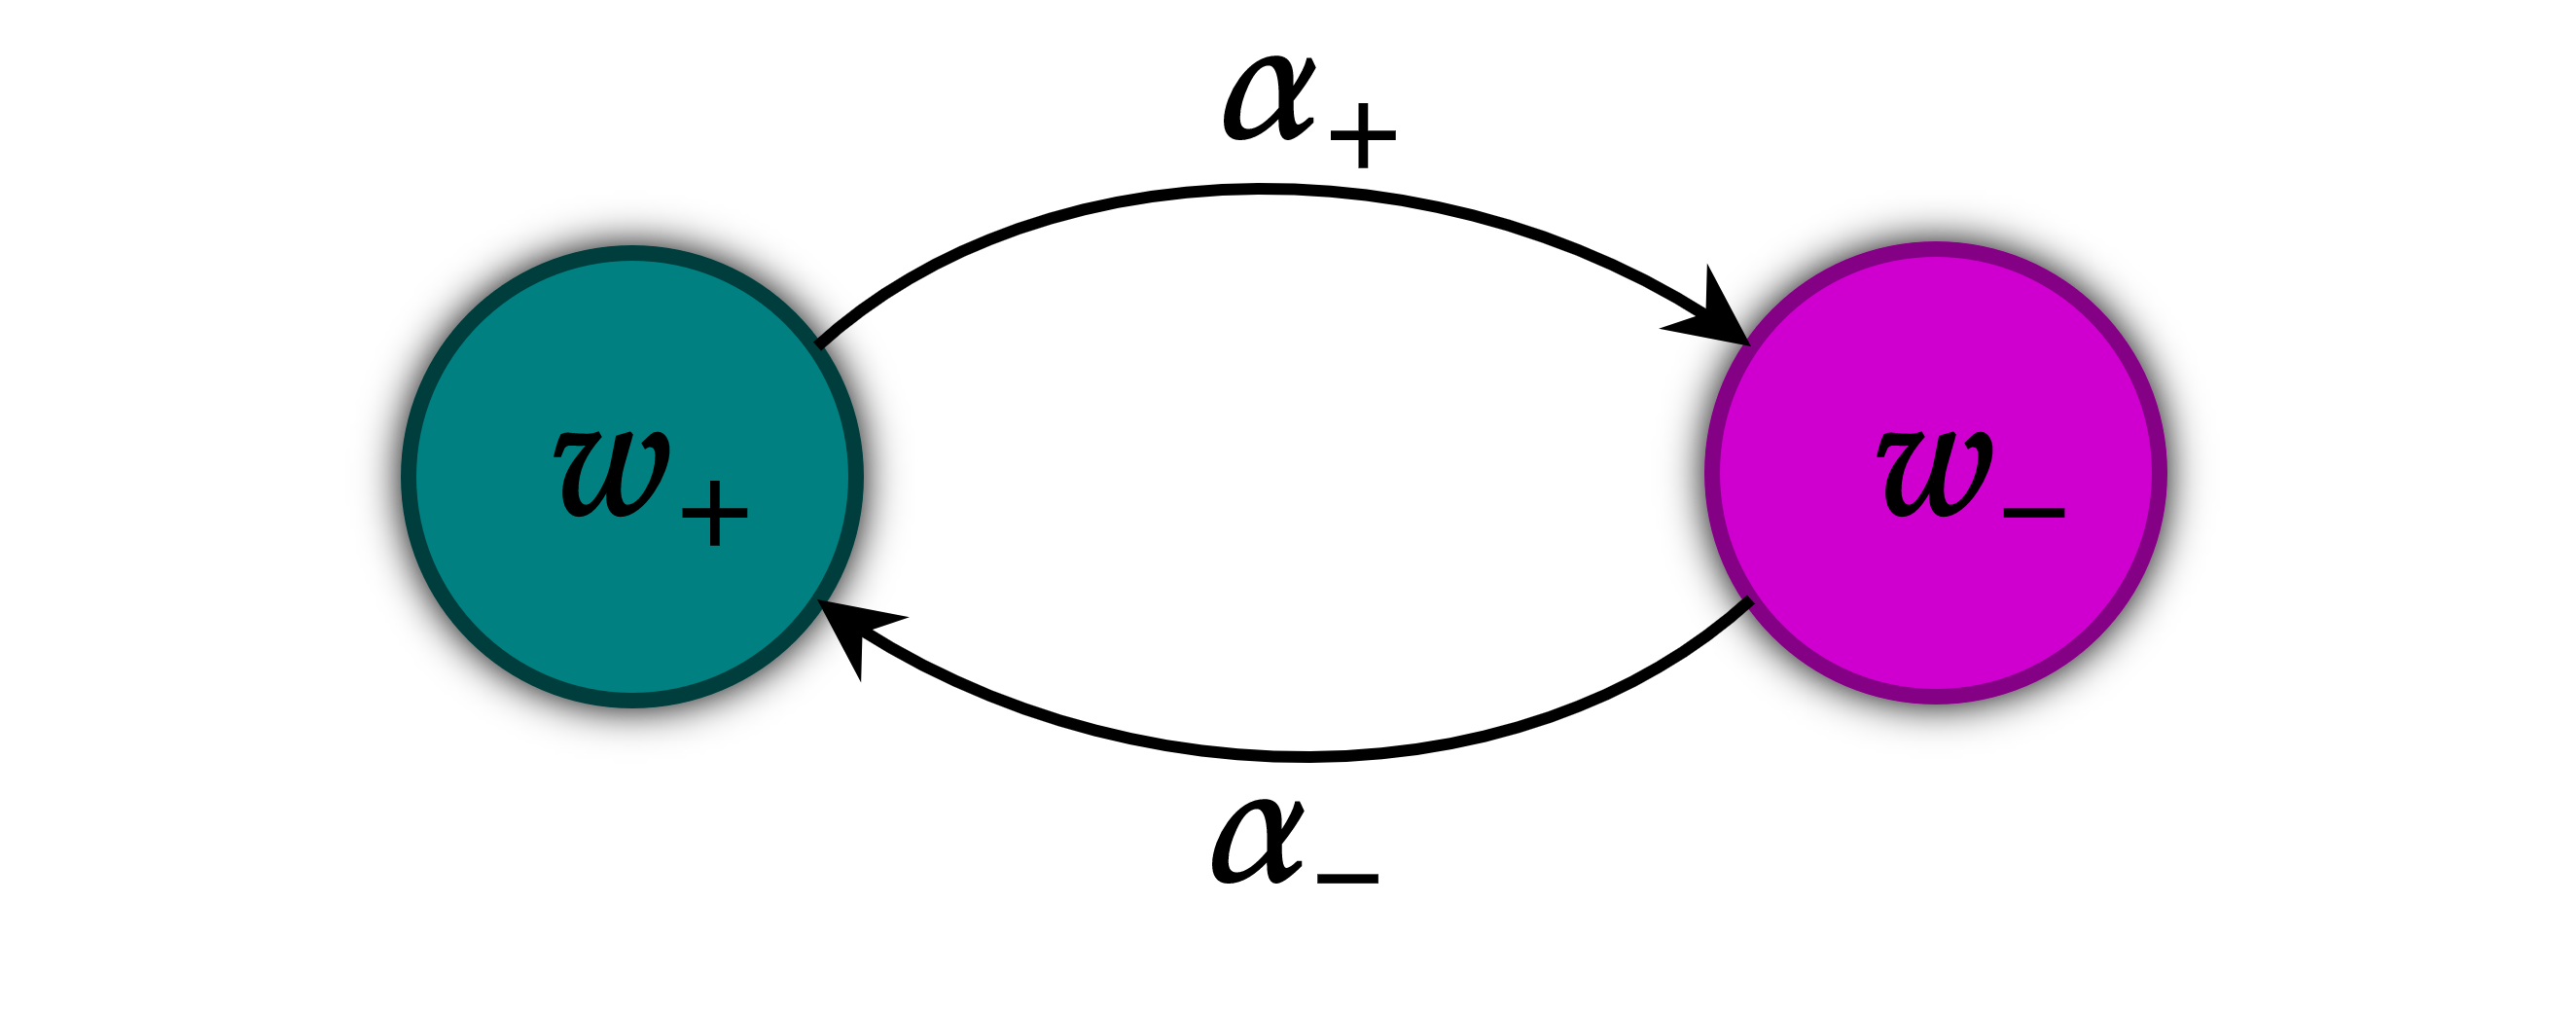
\includegraphics[width = 0.49\textwidth]{figures/tele-diagram-w3.png}}
\hfill
\subfloat[A Sample path for the asymmetric RnT particle.\label{sample_path}]{%
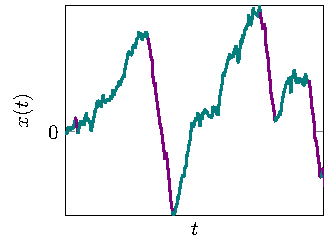
\includegraphics[width = 0.49\textwidth]{figures/RnT_sample_path.pdf}
}
\caption{\footnotesize Subfigure \ref{telegraph_diagram} shows a diagram of the telegraph process $w(t)$ as discussed in Subsection \ref{subsection:asymmetric-RnT}. In the +ve state, the particle has self-propulsion $\nu w_+$, and in the -ve state the self-propulsion is $\nu w_-$. Since $\Overline{w} = 0$, we have $\alpha_+w_- + \alpha_-w_+ = 0$. Subfigure \ref{sample_path} depicts a sample path for the particle governed by (\ref{main-langevin}) where $w(t)$ is an asymmetric telegraph process with zero mean. The green and purple line segments indicates the state of the driving telegraph process, corresponding to velocities $w_+$ and $w_-$ respectively. For this sample path we have set $\abs{w_-/w_+}= 5$.}
\label{figure1}
\end{figure}

According to Eqn. (\ref{zero-mean-entropy}), the leading order contribution to the entropy production rate of $x_t$ is 

\begin{align}\label{RnT-entroppy-int}
\entpp = \frac{\nu^6}{24TD^3}\int_0^T \rmd t_1 \rmd t_2 \rmd t_3 \left(\Overline{w(t_1)w(t_2)w(t_3)}\right)^2. 
\end{align}

In order to calculate the three-time correlation $\Overline{w(t_1)w(t_2)w(t_3)}$, begin from the master equation for the evolution of $w(t)$, 

\begin{equation}
\frac{\rmd}{\rmd t}\begin{pmatrix}
p_+(t) \\
p_-(t)
\end{pmatrix} =
\begin{pmatrix}
-\alpha_+ & \alpha_- \\
\alpha_+  & -\alpha_-
\end{pmatrix}
\begin{pmatrix}
p_+(t) \\
p_-(t)
\end{pmatrix}.
\end{equation}

Here $p_+(t)$ is the probability of the event $w(t) = w_+$ and $p_-(t)$ is the probability of the event $w(t) = w_-$. Solving this system with appropriate boundary conditions, one obtains the propagators  

\begin{equation}\label{elements}
    \begin{split}
        P_{++}(t) &= \frac{1}{\alpha_+ + \alpha_-} \left(\alpha_- + \alpha_+ e^{-(\alpha_+ + \alpha_-)t}\right) \\
        P_{-+}(t) &= \frac{1}{\alpha_+ + \alpha_-} \left(\alpha_+ - \alpha_+ e^{-(\alpha_+ + \alpha_-)t}\right) \\
        P_{+-}(t) &= \frac{1}{\alpha_+ + \alpha_-} \left(\alpha_- - \alpha_- e^{-(\alpha_+ + \alpha_-)t}\right) \\
        P_{--}(t) &= \frac{1}{\alpha_+ + \alpha_-} \left(\alpha_+ + \alpha_- e^{-(\alpha_+ + \alpha_-)t}\right) \\
    \end{split}
\end{equation}
where $P_{ij}(t)$ is the probability of $w(t)$ taking a value $w_i$ having been initialised at $t=0$ with value $w_j$, for $i,j \in \{+ , -\}$. The three-time correlation function of $w(t)$ is then 

\begin{equation}\label{3time}
\begin{split}
    \Overline{w(t_3)w(t_2)w(t_1)} =& \mathds{1}_{\{t_3>t_2>t_1\}}
 \begin{pmatrix}
1 & 1\\
\end{pmatrix}
M_{w}(t_3-t_{2})M_{w}(t_2-t_{1})
\begin{pmatrix}
w_+P_{+}\\
w_-P_{-}
\end{pmatrix}\\
&+\mathds{1}_{\{t_2>t_3>t_1\}}
 \begin{pmatrix}
1 & 1\\
\end{pmatrix}
M_{w}(t_2-t_{3})M_{w}(t_3-t_{1})
\begin{pmatrix}
w_+P_{+}\\
w_-P_{-}
\end{pmatrix} + \cdots
\end{split}
\end{equation}

where $P_{+/-}=\lim_{t \to \infty} P_{++/--}(t)$ are the stationary probabilities of $w(t)$ taking the value $w_{+/-}$ and $\mathds{1}_{\{t_3>t_2>t_1\}}$ are indicator functions which impose time-ordering. The transition matrix $M_w(t)$ is given by 

\begin{align}
    M_{w}(t) &= \begin{pmatrix}
w_+P_{++}(t) & w_+P_{+-}(t) \\
w_-P_{-+}(t)  & w_-P_{--}(t)
\end{pmatrix} \\ 
&= M_{w0} + M_{w1}e^{-(\alpha_+ + \alpha_-)t},
\end{align}

where 
\begin{align}
\begin{split}
M_{w0} &= \frac{1}{\alpha_+ + \alpha_-} \begin{pmatrix}
        w_+\alpha_- & w_+\alpha_- \\
        w_-\alpha_+ & w_-\alpha_+
        \end{pmatrix} \\
        M_{w1} &= \frac{1}{\alpha_+ + \alpha_-} \begin{pmatrix}
        w_+\alpha_+ & -w_+\alpha_- \\
        -w_-\alpha_+ & w_-\alpha_-
        \end{pmatrix}.
\end{split}
\end{align}

Eqn. (\ref{3time}) can be simplified using the relation 

\begin{equation}\label{3time2}
     \begin{pmatrix}
1 & 1\\
\end{pmatrix}M_{w0} = M_{w0}
\begin{pmatrix}
w_+P_{+}\\
w_-P_{-}
\end{pmatrix} = 0.
\end{equation}

The three-time correlation $\Overline{w(t_1)w(t_2)w(t_3)}$ is then given by 

\begin{equation}
\begin{split}
        \Overline{w(t_3)w(t_2)w(t_1)} &= \mathds{1}_{\{t_3>t_2>t_1\}}
 \begin{pmatrix}
1 & 1\\
\end{pmatrix}
M_{w1}^2
\begin{pmatrix}
w_+P_{+}\\
w_-P_{-}
\end{pmatrix} e^{-(\alpha_+ + \alpha_-)(t_3-t_1)} +  \\ &\quad \quad \mathds{1}_{\{t_2>t_3>t_1\}}
 \begin{pmatrix}
1 & 1\\
\end{pmatrix}
M_{w1}^2
\begin{pmatrix}
w_+P_{+}\\
w_-P_{-}
\end{pmatrix} e^{-(\alpha_+ + \alpha_-)(t_2-t_1)}\\
&= \frac{\alpha_+ \alpha_- (\alpha_+ w_+ + \alpha_- w_-)(w_+ - w_-)^2}{(\alpha_+ + \alpha_-)^3}\times \\ &\quad \quad \Big[ e^{-(\alpha_+ + \alpha_-)(t_3-t_1)}\mathds{1}_{\{t_3>t_2>t_1\}} + e^{-(\alpha_+ + \alpha_-)(t_2-t_1)}\mathds{1}_{\{t_2>t_3>t_1\}} + \cdots \Big]
\end{split}
\end{equation}

Using this expression in Eqn. (\ref{RnT-entroppy-int}), we obtain

\begin{align}
    \begin{split}
     \dot{\mathcal{S}}=  \frac{\nu^6}{4\cdot3!\cdot T D^3}\Bigg[\frac{\alpha_+ \alpha_- (\alpha_+ w_+ + \alpha_- w_-)(w_+ - w_-)^2}{(\alpha_+ + \alpha_-)^3}\Bigg]^2 \int_0^T\rmd t_1\rmd t_2\rmd t_3\Big[ & e^{-(\alpha_+ + \alpha_-)(t_3-t_1)}\mathds{1}_{\{(t_3>t_2>t_1\}} \\&+ e^{-(\alpha_+ + \alpha_-)(t_2-t_1)}\mathds{1}{\{t_2>t_3>t_1\}} + \cdots \Big]^2,
\end{split}
\end{align}

which evaluates to
\begin{align}
    \begin{split}
 \dot{\mathcal{S}}&=  \frac{\nu^6}{4\cdot3!\cdot T D^3}\Bigg[\frac{\alpha_+ \alpha_- (\alpha_+ w_+ + \alpha_- w_-)(w_+ - w_-)^2}{(\alpha_+ + \alpha_-)^3}\Bigg]^2\cdot 6 \int_0^T\rmd t_3\int_0^{t_3}\rmd t_2\int_0^{t_2}\rmd t_1  e^{-2(\alpha_+ + \alpha_-)(t_3-t_1)}\\
 &=\frac{\nu^6}{16 T D^3}\cdot \frac{\alpha_+^2 \alpha_-^2 (\alpha_+ w_+ + \alpha_- w_-)^2(w_+ - w_-)^4}{(\alpha_+ + \alpha_-)^8}
\end{split}
\end{align}

Finally, we use the zero-mean condition (\ref{zero-mean}) to obtain 

\begin{align}\label{RnT-ent}
\dot{\mathcal{S}}=-\frac{\nu^6}{16D^3}\cdot\frac{w_+^3w_-^3}{\alpha_+\alpha_-}\left(\frac{\alpha_+-\alpha_-}{\alpha_+ + \alpha_-}\right)^2
\end{align}

We may furthermore define the geometric average transitions rate $\bar{\alpha}= \sqrt{\alpha_+\alpha_-}$ and the geometric average speed $\bar{\omega} = \sqrt{\abs{w_+w_-}}$ to arrive at 

\begin{align}
  \dot{\mathcal{S}} = \frac{\nu^6}{16D^3}\frac{\bar{w}^6}{\bar{\alpha}^2}\left(\frac{1-\lambda}{1+\lambda}\right)^2,
\end{align}

where 

\begin{equation}
  \lambda \coloneqq \abs{\frac{w_-}{w_+}} = \frac{\alpha_-}{\alpha_+}.
\end{equation}

\subsection{Discussion}
\subsubsection{Entropy Production Results}

In Subsection \ref{methods} we present a perturbative framework for calculating the entropy production of self-propelling particles subject to a potential. In general, obtaining a closed form expression may be difficult when using this framework. However, in particular cases of interest, such as when the net current is zero, the calculations simplify considerably, allowing us to obtain closed-form expressions for the leading order contributions to entropy production.

In Subsection \ref{subsection:asymmetric-RnT} we derive the leading order contribution to the entropy production for a free asymmetric RnT particle. This is given by

\begin{equation}\label{RnT-ent-geom}
  \dot{\mathcal{S}} = \frac{\nu^6}{16D^3}\frac{\bar{w}^6}{\bar{\alpha}^2}\left(\frac{1-\lambda}{1+\lambda}\right)^2,
\end{equation}

where $\bar{w} = \sqrt{\abs{w_+w_-}}$ and $\bar{\alpha} = \sqrt{\alpha_+\alpha_-}$ are the geometric average speed and transition rate respectively, and

\begin{equation}
  \lambda \coloneqq \abs{\frac{w_-}{w_+}} = \frac{\alpha_-}{\alpha_+}.
\end{equation}

Eqn. (\ref{RnT-ent-geom}) illuminates the dependence of $\dot{\mathcal{S}}$ on the ratio of the speeds, $\lambda$. The entropy production disappears at $\lambda = 1$ as expected. For fixed values of $\bar{w}$ and $\bar{\alpha}$ the maximum entropy production

\begin{equation}\label{max_entropy}
  \dot{\mathcal{S}}_{\text{max}} = \frac{\nu^6}{16D^3}\frac{\bar{w}^6}{\bar{\alpha}^2}
\end{equation}

is achieved in the limit as $\lambda \rightarrow \infty$. This is consistent with the `Unexpected state mechanism' which we subsequently propose in Subsection \ref{EPmechanism}. The limit as $\lambda \rightarrow 0$ requires careful treatment. If this limit is taken by keeping $w_+, \alpha_+$ fixed and sending $w_-,\alpha_- \rightarrow 0$, then the resulting process will have zero entropy production. If, on the other hand the limit $\lambda \rightarrow 0$ is taken by fixing $w_-$ and sending $w_+ \rightarrow \infty$, the resulting process tends towards infinite entropy production. When $\lambda = 0$, we have that in the stationary state 
$\mathcal{P}\left[w(t) = w_-\right] = 1$, and hence as $w(t)$ approaches its equilibrium state, $x(t)$ behaves as an unforced Brownian motion with zero entropy production.

In the strong diffusion regime where $D \gg \bar{w}^2/\bar{\alpha}$, the noise dominates the self-propulsion kinetics and the entropy production disappears. In other words, the entropy production becomes negligible whenever $\bar{\alpha} \gg \bar{w}^2/D$. The factor $\bar{w}^2/D$ is analogues to the $v^2/D$ term which appears in the entropy production of a diffusion process with constant self-propulsion speed $v$\cite{cocconi2020entropy}. When the condition $\bar{\alpha} \gg \bar{w}^2/D$ is satisfied, the high transition rate effectively masks the self-propulsion of the particle, resulting in reduced entropy production.

\subsubsection{Entropy Production Mechanism}\label{EPmechanism}

\begin{wrapfigure}{R}{0.5\textwidth}
    \centering
    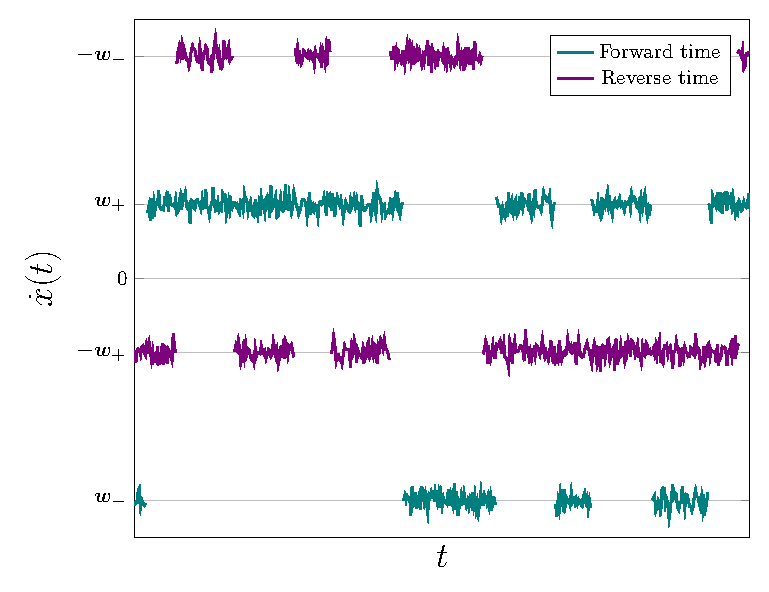
\includegraphics[width = 0.45\textwidth]{figures/unexpected_state.pdf}
    \caption{\footnotesize The observed velocities for a sample path of the asymmetric RnT process when time is run forwards (green/blue) and backwards (purple). Entropy production arises because time reversal results in the `unexpected' states $-w_-$ and $-w_+$ for the velocity. Maintaining these states has a high probability cost in terms of the noise, hence the different statistics of forward and reverse paths. Note that the forward path is simply the sum of a telegraph process and white noise, so it is time reversible. It is precisely the appearance of unexpected velocity states under time reversal that results in entropy production.} 
   \label{unexpeced_states}
\end{wrapfigure}

We have shown that the process $x(t)$ defined by (\ref{main-langevin}) has non-zero entropy production in its steady-state, even when $w(t)$ is hidden from the observer. However, the underlying telegraph process, $w(t)$, and white noise, $\xi(t)$, \textit{are} time reversible. Explicitly, the process defined by

\begin{equation}
\dot{y}(t) = \nu w(T-t) + \xi(T-t), \quad y(0) = 0, t \in [0, T]
\end{equation}

 has identical statistics to the process defined by (\ref{main-langevin}).  This provokes the following question: how can time-reversible underlying processes give rise to trajectories which are \textit{distinguishable} from their time-reverse? 
 The answer lies in the physical variables to which the processes are coupled. In equation (\ref{main-langevin}), the telegraph process represents a velocity. When time is reversed, not only is the trajectory of the telegraph process reversed, but also the sign of the velocity associated with that state. The result is the appearance of the `unexpected' states $-w_-$ and $-w_+$ in the velocity profile of the particle (figure \ref{unexpeced_states}). These unexpected states can only be maintained through persistent noise against the self-propulsion direction, which incurs a high probability cost according to Eqn. (\ref{varphi-cond-prob}). Put another way, the entropy production of the asymmetric RnT process results from the identity\footnote{This identity is only formal, since $x(t)$ is a.s. not differentiable. It can be interpreted as a statement about the increments of $x(t)$.}

\begin{equation}
\frac{\rmd x}{\rmd s}(s) = -\dot{x}(t),
\end{equation}

where $s = T-t$ is the reverse-time variable. But $-\dot{x}(t)$ does not result from the time reversal of the underlying mechanisms, i.e., the processes $x(s)$ and $y(t)$ are not equal in law. This observation emphasises the need to distinguish between the effect of time-reversal on the time-dependent parts of the dynamics (e.g. telegraphic noise) and the nature of the states themselves, which change in a time-independent way.




\section{Classification of Non-Markov Processes}\label{chapter:classification}
\textit{\textbf{Notational Warning:} In this section $\Omega$ no longer refers to the path space of a stochastic process. Instead, $(\Omega, \mathcal{F}, \bP)$ refers to a generic probability space}

\textit{In this section we conclude the text with a reflection on the nature of the stochastic processes considered. We propose a novel classification of non-Markov processes to guide future research in the area. It is hoped also that the following discussion can help to bridge the gap between the mathematical discipline of Stochastic Processes and the study of such processes in physics.}

By way of reflection and to motivate future study, It is pertinent to present a classification of the types of non-Markov processes considered here. Such a classification is helpful because the class of processes that can be considered non-Markov is very broad. Throughout Sections \ref{chapter:telegraph}-\ref{chapter:RnT} we have developed techniques for analysing processes that fall within the different categories described in this section. In this way, the following categorisation can also guide future work on non-Markov stochastic processes by helping to identifying useful techniques in each case. In the sequel, we shall assume $\mathcal{X}$ to be a \emph{Polish} space (meaning that $\mathcal{X}$ allows a seperable and complete metrisation) and that it is endowed with its Borel $\sigma$-algebra. First, let us recall that a Markov process $X_t: \Omega \times [0,+\infty) \rightarrow \mathcal{X}$, is one that satisfies 

\begin{align}\label{Markov-property}
\bE[f(X_t) \lvert \mathcal{F}_s] = \bE[f(X_t) \lvert X_s], \quad s \leq t.
\end{align}

Here $\mathcal{F}_t = \sigma \left(\{X_s: \, s \leq t \}\right)$ is the $\sigma$-algebra generated by $X_t$ up to time $t$ and $f: \mathcal{X} \rightarrow \bR$ is any bounded measurable function. The classifications that follow are not meant for dividing non-Markov processes into mutually exclusive groups. Indeed, if a process fulfils one classification that does not preclude it from satisfying also the others. Instead, these groupings identify unifying paradigms that will be helpful in the study of non-Markov processes in future.

\subsection{Quasi-Markov Processes}
To motivate this first category, consider the following example from \cite{XuMeiMarkov}. Let $\{Y_n\}_{n=0}^\infty$ be i.i.d random variables taking value in $\{1,2,\ldots, 20\}$. Define $x_0 = Y_0$, $x_1 = Y_1$, and $x_{n+1} = x_n + x_{n-1} + Y_{n+1}$ for $n \geq 1$. Also define $z_n = (x_n, x_{n-1})$. It is easily checked that $x_n$ is not Markov -for example $x_2$ depends on $x_0$ and $x_1$ which are themselves independent- while $z_n$ is Markov. In this example, the non-Markov nature of $x_n$ is rather trivial. It is a matter of description. The process can be made Markov by simply keeping a record of its history up to a constant time before the present. This is achieved with the r.v. $z_n$. 

More generally, let $T \in [0, \infty)$ be a constant time. Define the future of $X_t$, $\mathcal{F}_t^\ast = \sigma\left(\{X_s: s \geq t\}\right)$. Let $X_t$ be a process satisfying 

\begin{align}\label{quasi-Markov}
\bE[f(X_t) \lvert \mathcal{F}_s] = \bE[f(X_t) \lvert \mathcal{F}^\ast_{s-T}\cap\mathcal{F}_s], \quad T \leq s.
\end{align}

We shall refer to processes satisfying Eqn. (\ref{quasi-Markov}) for some $T$ as quasi-Markov processes. The process $x_n$ defined above is a discrete-time quasi-Markov process. Other examples of quasi-Markov processes include time-delayed DEs and Stochastic Differential Delay Equations (SDEEs). For a quasi-Markov process $X_t$, we define the \textit{Markov description} of $X_t$,

\begin{align}\label{Markov-description}
Z_t \coloneqq \left \{X_s\right\}_{s=t}^{t+T} : \Omega \times [0, +\infty) \rightarrow \mathcal{X}^{[0,T]}.
\end{align}

As the name suggests, $Z_t$ is a Markov process. In general it is an infinite dimensional process, but for discrete-time processes it is $T$-dimensional. In the first motivating example for this section, $z_n$ is the Markov description of $x_n$. What we call the Markov description of $X_t$ has been implicitly used to study systems with delayed dynamics using the framework of functional differential equations\cite{kolmanovskii2013introduction,richard2003time}.  When $T = 0$, then $\mathcal{F}^\ast_{s-T}\cap\mathcal{F}_s = \sigma(\{X_s\})$, hence Eqn. (\ref{quasi-Markov}) becomes 

\begin{align}
\bE[f(X_t) \lvert \mathcal{F}_s] = \bE[f(X_t) \lvert X_s], 
\end{align}

so $X_t$ is Markov. We have not not considered any quasi-Markov systems in the preceding sections, nevertheless they comprise an important category of non-Markov processes. 

\subsection{Semi-Markov Processes}
By way of comparison with a quasi-Markov process, consider the `Waiting Room' (WR) process described in Section \ref{chapter:waiting-room}. Refer to Section \ref{chapter:waiting-room} for a full description of this process. Here we let $R_t$ denote the WR process. The state-space for this process is $\mathcal{X} = \{\ket{1},\ket{3}, \ket{w(t)} = a(t)\ket{2} + b(t)\ket{4} \}$ where $0<a(t),b(t)<1$ and $a(t)+b(t) =1$. Whenever the system occupies states $\ket{1}$ or $\ket{3}$, its evolution is independent of the past. However, when the system occupies $\ket{w}$ its time evolution depends on the past up to the last instance when either of the states $\ket{1}$ or $\ket{3}$ were observed (see Eqn. (\ref{waiting-room-timeevol})). In this case, if we were to use all available information to predict the future of $R_t$, our record keeping would need to extend until the first such instance. But how long ago the process occupied either of $\ket{1}$ or $\ket{3}$ is itself a stochastic variable. This is unlike the first example with the process $x_n$. In the case of $x_n$ the time-evolution of the process is affected by a \textit{constant} time-delay. The time-delay in the case of $R_t$ varies stochastically. 

We now let $T$ be a stopping time with respect to the filtration $\{\mathcal{F}_t\}_{t=0}^\infty$. A stopping time\newline $T: \Omega \rightarrow [0, +\infty]$ with respect to $\{\mathcal{F}_t\}_{t=0}^\infty$ is a random variable such that the event $\{T \leq t\}$ is $\mathcal{F}_t$ measurable for all $t$. The stopped $\sigma$-algebra of $X_t$ with respect to $T$ is the set 

\begin{align}
\mathcal{F}_T = \left\{A \in \mathcal{F}_\infty : A \cap \{T \leq t\} \in \mathcal{F}_t, \quad \forall t > 0\right\}\end{align}

Intuitively, $\mathcal{F}_T$ is comprised of all the information about the process $X_t$ up to time $T$. Suppose that $T$ is almost surely finite, $\bP( T < \infty) = 1$. Then we will say that $X_t$ is a semi-Markov process if

\begin{align}\label{semi-Markov-property}
\bE[f(X_{T+t})\lvert\mathcal{F}_T] =  \bE[f(X_{T+t}) \lvert X_T].
\end{align}

for some stopping time $T$. When Eqn. (\ref{semi-Markov-property}) holds for all stopping times $T$ with respect to $\{\mathcal{F}_t\}_{t=0}^\infty $, then $X_t$ is said to have the strong Markov property \cite{durrett2019probability} which is a stronger formulation of the Markov property (Eqn. (\ref{Markov-property})). When a semi-Markov process is restarted at time $T$, then its future, conditioned on the present, is independent of the past. As we shall see in Section \ref{chapter:waiting-room}, a useful technique when considering semi-Markov processes is to restrict to the stopped process $X_{\min(t,T)}$. Since we can think of the process as restarting after time $T$, many quantities of interest are captured adequately by $X_{\min(t,T)}$. 

The WR process is a semi-Markov process. Let 

\begin{align}
T_1 = \inf \{t \geq 0: R_t = \ket{1}\}.
\end{align}

Since the Poisson jump rates away from $\ket{1}$ are independent of how the process came to this state, the semi-Markov property 

\begin{align}
\bE[f(R_{T_1+t})\lvert\mathcal{F}_{T_1}] =  \bE[f(R_{T_1+t}) \lvert R_{T_1} = \ket{1}],
\end{align}

holds. Likewise $R_t$ also obeys the semi-Markov property with respect to the stopping time 

\begin{align}
T_3 = \inf\{ t \geq 0: R_t = \ket{3}\}.  
\end{align}

\subsection{Lego Brick Processes}
 In Section \ref{chapter:UL1} we derive the path probabilities of the `Unrequited Love' (UL) system. This is a two-state Poisson process where the jump rate depends on the state of another Poisson process. We begin with a continuous-time Markov chain taking values in   $\{\ket{11},\ket{12},\ket{21},\ket{22}\}$ and driven by the master equation
 
 \begin{align}
\dot{P}(t) = e^{tW}P(t), \; \; \;  W = \begin{pmatrix} -\alpha - \beta & \alpha & \beta + \gamma & 0 \\
  \alpha & -\alpha -\beta -\gamma & 0 & \beta \\
  \beta & 0 & -\alpha-\beta-\gamma & \alpha \\
  0 & \beta+\gamma & \alpha & -\alpha-\beta\end{pmatrix},
\end{align}

where $\alpha$, $\beta$, and $\gamma$ are positive constants. With respect to the phase space, $W$ has the basis ordering $e_1 = \ket{11}$, $e_2 = \ket{21}$, $e_3 = \ket{12}$, and $e_4 = \ket{22}$, so that, for example, $W_{12}$ is the rate for the transition $\ket{21} \rightarrow \ket{11}$. Denote this Markov-chain by $Z_t$. We then collapse the state $\ket{11}$ into $\ket{12}$ to obtain the coarse-grained state $\ket{1}$. We also collapse $\ket{21}$ with $\ket{22}$ to obtain $\ket{2}$. The resulting two-state process, denoted henceforth by $U_t$, is the UL system. See Section \ref{chapter:UL1} for a more thorough description. 

The process $U_t$ is non-Markov. Indeed, the time spent by $U_t$ in either of the states $\ket{1}$ or $\ket{2}$ informs the observer of the underlying state of $Z_t$. The transition probabilities for $U_t$ are then updated based on the inferred state of $Z_t$. $U_t$ can be viewed as the coupling of two Poisson process in the following sense. Let $N_t$ be a symmetric telegraph process with rate $\alpha$ taking values in $ \{0,\gamma\}$. Then for small time $\delta t$

\begin{align}
\begin{split}
\bP\left(U_{t+\delta t} = \ket{i} \: \lvert \: U_t = \ket{j}, N_t = n  \right) = (\beta + n)\delta t, \quad i \neq j.
\end{split}
\end{align}


This is equivalent to 


\begin{align}
\begin{split}
\bE\left(f\left(U_{t+\delta t}\right)\: \lvert \: U_t = \ket{j}, N_t = n  \right) = f\left(\ket{i}\right)(\beta + n)\delta t - f\left(\ket{j}\right)(1 - (\beta + n)\delta t) , \quad i \neq j.
\end{split}
\end{align}

In other words, the generator of the process $U_t$ is a function of $N_t$. It is in this sense that we speak of the coupling of processes. In Section \ref{chapter:UL1} we were interested in the case where $Y_t$ is hidden fom the observer, meaning the situation where all available information is contained in the filtration generated by $U_t$. In general, let $(X_t,Y_t): \Omega \times [0, +\infty) \rightarrow \mathcal{X}\times \mathcal{Y}$ be a random variable such that $(X_t,Y_t)$ is Markov and moreover, for any $g: \mathcal{Y} \rightarrow \bR$ measurable there holds

\begin{align}
\bE[g(Y_t) \: \lvert \: \sigma(\{X_u,Y_u: u \leq s\})] &= \bE[g(Y_t) \:\lvert \:Y_s], \\
\bE[f(X_t) \: \lvert \sigma(\{X_u,Y_u: u \leq s\})]  &= \bE[f(X_t) \:\lvert \: \sigma(X_s,Y_s) ],
\end{align}

for all $s \leq t$. Such a process we call a `Lego Brick' process (thinking of processes as Lego bricks, $X_t$ is built on top of $Y_t$). The non-trivial cases are those where $\bE[f(X_t) \:\lvert \: \sigma(X_s,Y_s) ] \neq \bE[f(X_t) \:\lvert \: X_s ]$. Identifying $(U_t, N_t)$ with $(X_t, Y_t)$ as in the above, the UL processes is a Lego brick process. Recall the asymmetric RnT process described in Section \ref{chapter:RnT},
\begin{align}
dx_t = w_t \rmd t + \sqrt{2D}dB_t
\end{align}

where $B_t$ is Brownian motion and $w(t,\omega)$ is a stochastic process with bounded measurable sample paths. Here $(x_t, w_t)$ is a Lego brick process. Considering again the generic process $(X_t, Y_t)$, let us call $X_t$ the `follower' (process) and $Y_t$ the `leader' (process). In general, the paths of the follower become non-Markov in the absence of information about the leader. The most intuitive approach in dealing with this complication is to integrate over the paths of the leader. Indeed, this has been our approach in Sections \ref{chapter:UL1} and \ref{chapter:RnT}. This technique makes implicit use of the following proposition from Probability Theory \cite{XueMeiAltman2020}.\footnote{See Appendix A, Proposition A.5 for a proof of this statement.}

\begin{prop} 
Let $X: \Omega \rightarrow \mathcal{X}_1$ be $\mathcal{F}^\prime \subset \mathcal{F}$ measurable and let $Y: \Omega \rightarrow \mathcal{Y}$ be independent of $\mathcal{F}^\prime$. Let $\psi: \mathcal{X}\times \mathcal{Y} \rightarrow \bR$ be $\mathcal{B}(\mathcal{X}) \times \mathcal{B}(\mathcal{Y})$ measurable such that $\bE \abs{\psi(X,Y)} < \infty$. Define $h_\psi(x) \coloneqq \bE[\psi(x,Y)] = \int_\Omega \psi(x,Y(\omega)) \rmd\bP(\omega)$. Then 

\begin{align}
\bE\left[\psi(X,Y) \: \lvert \: \mathcal{F}^\prime\right] = h_\psi(X).
\end{align}
\end{prop}

To apply this result to our generic Lego brick process we identify

\begin{align}
\begin{split}
X &\longleftrightarrow \bE\left[X_t \: \lvert \: X_s \right] \\
Y &\longleftrightarrow \bE\left[Y_t \: \lvert \: Y_s \right] \\ 
\mathcal{F}^\prime &\longleftrightarrow \sigma(X_s).
\end{split}
\end{align}
\section{Conclusion}

The entropy production rate of non-equilibrium systems has been the subject of growing interest in the Stochastic Thermodynamics literature. Theoretical results regarding the entropy production of non-Markov processes have been developed. However, to date no paradigmatic, exactly solvable non-Markov models have appeared in the literature. In order to develop such a model, we investigate the path probabilities and entropy production rate of some candidate systems. 

A path-space formulation for continuous-time, discreet-space Markov chains is developed and validated through recovering the fully time-dependent probability flow and entropy production rate of the telegraph process. To the author's knowledge, this is the first derivation of a closed-form expression for the entropy production of any processes in a path-space framework in the literature on entropy. Although the additional difficulty involved in path-space analysis make this framework inadvisable for dealing with simple Markov chains, the path-space formulation is crucial in the investigation of non-Markov processes where entropy production can arise from asymmetric waiting-time distributions. Hence, the validation of this path-space formulation is an important result for the literature. 

The path-space framework is applied to a coarse-grained Markov chain (the `Waiting Room')  whereby an analytic, closed-form result for the entropy production rate of a non-Markov process is derived. Such a paradigmatic, exactly-solvable non-Markov model represents a step forward for the Stochastic Thermodynamics literature. The entropy production rate for the Waiting Room system is compared with that of the corresponding Markov chain and found to exhibit a number of unexpected features. In particular, the two systems exhibit qualitatively different behaviours in the limits as the reverse rate of the process becomes large or small. The expressions obtained also confirm for these systems a well-established theoretical result regarding the upper bound on the entropy production rate of a coarse-grained process. Moreover, the entropy production of the coarse-grained and the granular systems are found to be due to distinct mechanisms. Hence, the process of coarse-graining is found to affect not only the quantity but also the nature of entropy production. 

We derive the path probabilities of another coarse-grained Markov chain (the `Unrequited Love' system). These probabilities are presented in terms of a generalised generating function . This problem serves well to illustrate the difficulties in analysing non-Markov paths even in relatively simple systems. The main sources of difficulty are the non-trivial dependence of `hidden' processes on observable quantities, and the scaling of pertubative corrections with the number of transitions along a path. 

Moving to a continuous-space setting, a perturbation theory is developed for the entropy production rate of diffusion processes with stochastic, time-dependent drift terms beginning from the relevant Onsanger-Machlup functional. Crucially, This perturbation theory applies in those cases where the process driving the drift term is hidden, i.e. when the observable process is non-Markov. This general perturbation theory is new for the literature. This theory is applied to an asymmetric Run-and-Tumble (RnT) particle and the leading order contribution to the entropy production rate of this process is derived in closed form. In principle, it allows the entropy production rate of a process to be calculated up to arbitrary order whenever its drift is small compared to its diffusion (meaning small $v^2/D$, where $v$ is the characteristic drift and $D$ is the diffusion constant). The entropy production result for the asymmetric RnT particle demonstrates how a system driven by reversible dynamics can give rise to entropy production due to the nature of the physical coupling involved. Inspired by this result, we propose the `Unexpected State' mechanism of entropy production. 

We conclude with a novel classification of non-Markov processes that is intended to identify unifying paradigms and guide future research. In this penultimate section the concrete problems considered previously are presented in an abstract setting more conducive to a Probability Theoretic approach. Likewise our approach to each problem is formulated as it would apply in a general setting. It is hoped that this discussion can begin to bridge the gap between the rapidly advancing theory of Stochastic Processes and the study of stochastic systems in Statistical Physics, in particular Stochastic Thermodynamics. 

In terms of immediate applicability to physical or biological systems, future work must focus on relating the mathematical results presented here back to the key physical concepts of heat, free energy, and work. Once these relationships have been established, experimental work is needed to verify these results in real systems. Future work concerned with the theory of entropy production can use the waiting room system as an anchor to derive the entropy production rate of more complex systems. The perturbation theory derived in Section $\ref{chapter:RnT}$ presents an interesting link with contemporary research in Stochastic Analysis, whereby the theory of rough paths may be invoked to explain how, and in what sense, smooth functions can be understood to approximate a Brownian sample path. 
\section*{Appendices}

\addcontentsline{toc}{section}{Appendices}
\renewcommand{\thesection}{\Alph{subsection}}
\setcounter{subsection}{0}
\subsection{Required Definitions, Theorems, and Lemmas}

We first give the following definition of a matrix function from \cite{higham2008functions}.
\label{appendix:lemmas}
\begin{definition}[Matrix function via Cauchy integral]
For $A \in \bC^{n\times n}$, 

\begin{align}
f(A) \coloneqq \frac{1}{2\pi i}\oint_\gamma f(z)(z\mathds{1} - A)^{-1} \, \rmd z, 
\end{align}

where $f$ is analytic on and inside a closed contour $\gamma$ that encloses the spectrum of $A$. 
\end{definition}

In the above, the integral is taken element-by-element. 

\begin{theorem}[Dominated Convergence Theorem]
Let $(\mathcal{X}, \mathcal{F}, \mu)$ be a measure space. If the sequence of functions $\{f_n\}$ converges pointwise to $f$ on $\mathcal{X}$ and furthermore there exists $\phi \in L^1(\mu)$ such that $\abs{f_n(x)} \leq \abs{\phi(x)}$ for all $x \in \mathcal{X}$ and for all $n$, then 

\begin{align}
\lim_{n\rightarrow \infty} \int_{\mathcal{X}} f_n \,\rmd \mu = \int_{\mathcal{X}} f \,\rmd \mu
\end{align}
\end{theorem}
\begin{proof}
See \cite[\S 44]{kolmogorov2012elements} or any introductory functional analysis textbook.
\end{proof}
\begin{corollary}\label{limit-of-mat}
Let $A \in \bC^{m\times m}$. Then $\lim_{n\rightarrow \infty}(\mathds{1}+\frac{1}{n}A)^n = e^A$.
\end{corollary}
\begin{proof}
Define $f_n(z) = (1 + z/n)^n$. Note that
\begin{equation}
  \abs{(1+\frac{z}{n})^n} \leq (1 + \abs{\frac{z}{n}})^n
\end{equation}

so for a contour $\gamma$ such that $\sup_{z \in \gamma} \abs{z} = M$, we have the inequality

\begin{equation}
  \abs{(1+\frac{z}{n})^n} \leq (1 + \frac{\abs{M}}{n})^n \uparrow e^M
\end{equation}

Now take $\gamma$ to be a simple, closed, positively oriented contour that encloses the spectrum of $A$. Then

\begin{equation}\label{integral_proof}
  (\mathds{1}+\frac{1}{n}A)^n = \frac{1}{2\pi i}\oint_\gamma f_n(\zeta)(\zeta \mathds{1} - A)^{-1}\: d\zeta.
\end{equation}
But $f_n(z) \rightarrow e^z$ pointwise and there exists $M \in \bR$ such that $|f_n| \leq e^M \in L^1(\gamma)$ for all $n$. Now take the limit of (\ref{integral_proof}) as $n \rightarrow \infty$ and apply the dominated convergence theorem to find that

\begin{equation}
\lim_{n\rightarrow \infty} (\mathds{1}+\frac{1}{n}A)^n = e^A
\end{equation}
\end{proof}

\begin{proposition}\label{mat-exp-lemma}
If $X$ is a traceless, $2 \times 2$ matrix, then

  $$ e^X = \cos \sqrt{\det X}\,\mathds{1} + \frac{\sin \sqrt{\det X}}{\sqrt{\det X}}X.$$
\end{proposition}
\begin{proof}
See \cite[\S 1.2]{WulfLiegroups}.
\end{proof}

\begin{proposition}\label{recursion-lemma}
  For $n = 0, 1 ,2 \ldots$, Let $I_n(t,r)$ be the integral

  \begin{equation}
    I_n(t,r)= \int_0^t dt_1\int_{t_1}^t dt_2\ldots \int_{t_{L-1}}^t dt_n \prod_{i \; \text{odd}}^n e^{rt_i} \prod_{i \: \text{even}}^n e^{-rt_i},
  \end{equation}

  with the convention $I_0 = 1$. Then we have the recurrence relation

  \begin{equation}\label{differential_recurrence_odd_proof}
    \dot{I}_{n+1}(t,r) = e^{-rt}  I_n(t,r); \; \; I_{n+1}(0,r) = 0
  \end{equation}

  for odd $n$ and

  \begin{equation}\label{differential_recurrence_even_proof}
    \dot{I}_{n+1}(t,r) = e^{rt}  I_n(t,r); \; \; I_{n+1}(0,r) = 0
  \end{equation}

  for even $n$.

\end{proposition}
\begin{proof}
We will show the odd $n$ case. The case for even $n$ is analogous. The base case $n=1$ is easily checked. For the induction, Note that

\begin{align}
  I_n(t,r) &= \int_0^t e^{rt_1}dt_1\int_{t_1}^t e^{-rt_2}dt_2\ldots \int_{t_{L-1}}^t e^{rt_n}dt_n \\
  &= \int_{[0,t]^n} \mathds{1}_{\{0 < t_1 < \ldots < t_n < t\}}e^{rt_1}e^{-rt_2}\ldots e^{rt_n} dt_n\ldots dt_1 \\
  &= \int^t_0 e^{rt_n} dt_n \ldots \int_0^{t_3}e^{-rt_2}dt_2\int_0^{t_2}e^{rt_1}dt_1.
\end{align}

Then

\begin{equation}\label{integral_recurrence}
  I_{n+1}(t,r) = \int_0^t e^{-rs} ds \int_0^s e^{rt_n} dt_n \ldots \int_0^{t_3}e^{-rt_2}dt_2\int_0^{t_2}e^{rt_1}dt_1 = \int_0^t e^{-rs} I(s,r)ds.
\end{equation}

Differentiating (\ref{integral_recurrence}) gives the result.
\end{proof}

\begin{proposition} 
Let $X: \Omega \rightarrow \mathcal{X}_1$ be $\mathcal{F}^\prime \subset \mathcal{F}$ measurable and let $Y: \Omega \rightarrow \mathcal{Y}$ be independent of $\mathcal{F}^\prime$. Let $\psi: \mathcal{X}\times \mathcal{Y} \rightarrow \bR$ be $\mathcal{B}(\mathcal{X}) \times \mathcal{B}(\mathcal{Y})$ measurable such that $\bE \abs{\psi(X,Y)} < \infty$. Define $h_\psi(x) \coloneqq \bE[\psi(x,Y)] = \int_\Omega \psi(x,Y(\omega)) \rmd\bP(\omega)$. Then 

\begin{align}
\bE\left[\psi(X,Y) \: \lvert \: \mathcal{F}^\prime\right] = h_\psi(X).
\end{align}
\end{proposition}

\begin{proof}
A proof of this theorem is given in \cite{XueMeiAltman2020}, but since this resource is not easily accessible we shall reproduce a modified version of the proof here. 

Let $\tilde{\psi}(x,y) = \mathds{1}_{A}(x)\mathds{1}_{B}(y)$ for $A \in \mathcal{B}(\mathcal{X}), \,B \in \mathcal{B}(\mathcal{Y}) $. Then since $X$ is $\mathcal{F}^\prime$ measurable and $Y$ is $\mathcal{F}^\prime$ independent we have 

\begin{align}
\bE\left[\tilde{\psi}(X,Y) \: \bigg\lvert \: \mathcal{F}^\prime\right] = \mathds{1}_A(X)\bE[\mathds{1}_B(Y)] = h_{\tilde{\psi}}(X).
\end{align}

This shows that $A \times B \in \mathcal{H}$ where 

\begin{align}
\mathcal{H} \coloneqq \left \{C \in \mathcal{B}(\mathcal{X})\times \mathcal{B}(\mathcal{Y}): \: \bE[\mathds{1}_C(X,Y) \: | \: \mathcal{F}^\prime] = h_{\mathds{1}_C}(X)  \right\}.
\end{align}

Indeed, letting $\mathcal{C} = \left\{A \times B: \: A \in \mathcal{B}(\mathcal{X}), \,B \in \mathcal{B}(\mathcal{Y})\right\}$, $\mathcal{C}$ is a $\pi$-system that generates $\mathcal{B}(\mathcal{X})\times \mathcal{B}(\mathcal{Y})$. Moreover the above shows that $\mathcal{C} \in \mathcal{H}$. It is simple to check that $\mathcal{H}$ is a $\lambda$-system. Then, by the $\pi-\lambda$ theorem, $\mathcal{H} = \mathcal{B}(\mathcal{X})\times \mathcal{B}(\mathcal{Y})$. Hence, the claim holds for all simple functions. Now, every $\psi: \mathcal{X}\times \mathcal{Y} \rightarrow \bR$ which is bounded and measurable is the uniform limit of a sequence of simple functions. Hence the claim holds for all $\psi$ by an application of the dominated convergence theorem for conditional expectations. 

\end{proof}

\subsection{Relating to the Unrequited Love Process}
\label{appendix:recovering}
In Chapter \ref{chapter:UL1} we propose a framework for summing over the nuisance paths of the leader particle to derive the marginal probability of the follower's path, $\bP(\omega_B)$.  Here we test the validity of the framework by using it to some over the nuisance paths of the follower to recover the behaviour of the leader particle. We will also explain in more detail the matrix algebra used in Section \ref{chapter:UL1}. 

\subsubsection{Matrix Algebra}
Let 
\begin{align}
M = \begin{pmatrix} M_1 & M_2 \\ M_3 & M_4\end{pmatrix}
\end{align}
where each $M_i$ is a $2 \times 2$ matrix of real numbers. Let us consider the inner product 

\begin{align}\label{inner-prod-sandwich}
\bP(\omega_B) = \frac{1}{2}\begin{pmatrix}1 \\ 1 \\ 0 \\ 0 \end{pmatrix}^T\begin{pmatrix} M_1 & 0 \\ M_3 & 0 \end{pmatrix}^{m_1-1}\begin{pmatrix} 0 & M_2 \\ 0 & M_4 \end{pmatrix}^{m_2}\ldots\begin{pmatrix} M_1 & 0 \\ M_3 & 0 \end{pmatrix}^{m_{L+1}-1}M\begin{pmatrix}1 \\ 1 \\ 0 \\ 0 \end{pmatrix}
\end{align}

as is done in Section \ref{chapter:UL1}. We compute 

\begin{align}
  \begin{pmatrix} M_1 & 0 \\ M_3 & 0 \end{pmatrix}^{m} =   \begin{pmatrix} M_1^m && 0 \\ M_3M_1^{m-1} & 0 \end{pmatrix} ,\quad \begin{pmatrix} 0 & M_2 \\ 0 & M_4 \end{pmatrix}^m = \begin{pmatrix} 0 & M_2M_4^{m-1} \\ 0 & M_4^m \end{pmatrix}.
\end{align}

Thus, 
\begin{align}
\begin{split}
  \begin{pmatrix} M_1 & 0 \\ M_3 & 0 \end{pmatrix}^{m}\begin{pmatrix} 0 & M_2 \\ 0 & M_4 \end{pmatrix}^n &=  \begin{pmatrix} M_1^m && 0 \\ M_3M_1^{m-1} & 0 \end{pmatrix}\begin{pmatrix} 0 & M_2M_4^{n-1} \\ 0 & M_4^n \end{pmatrix} \\ 
  &= \begin{pmatrix}0 & M_1^m M_2 M^{n-1}_4 \\ 0 & M_3M_1^{m-1}M_2M_4^{n-1} \end{pmatrix},
\end{split}
\end{align}

\begin{align}
\begin{split}
\begin{pmatrix} 0 & M_2 \\ 0 & M_4 \end{pmatrix}^n\begin{pmatrix} M_1 & 0 \\ M_3 & 0 \end{pmatrix}^{m} &= \begin{pmatrix} 0 & M_2M_4^{n-1} \\ 0 & M_4^n \end{pmatrix}\begin{pmatrix} M_1^m && 0 \\ M_3M_1^{m-1} & 0 \end{pmatrix}\\
&= \begin{pmatrix} M_2M_4^{n-1}M_3M_1^{m-1} & 0 \\ M_4^n M_3 M_1^{m-1} & 0\end{pmatrix},
\end{split}
\end{align}

\begin{align}
\begin{split}
  \begin{pmatrix} M_1 & 0 \\ M_3 & 0 \end{pmatrix}^{m}M &=   \begin{pmatrix} M_1^m & 0 \\ M_3M_1^{m-1} & 0 \end{pmatrix}\begin{pmatrix}M_1 & M_2 \\ M_3 & M_4\end{pmatrix}\\
  &= \begin{pmatrix}M_1^{m+1} & M_1^{m}M_2 \\ M_3M_1^{m} & M_3M_1^{m-1}M_2 \end{pmatrix}.
\end{split}
\end{align}

Combining these results, one partially evaluates the sandwiched matrix in Eqn. (\ref{inner-prod-sandwich}) to be 

\begin{align}
\begin{pmatrix}M_1 & 0 \\ M_3 & 0 \end{pmatrix}^{m_1-1}\begin{pmatrix} 0 & M_2 \\ 0 & M_4 \end{pmatrix}^{m_2}\ldots\begin{pmatrix} M_1 & 0 \\ M_3 & 0 \end{pmatrix}^{m_{L+1}-1}M = \begin{pmatrix}\Lambda & \ast \\
\ast & \ast \end{pmatrix},
\end{align}

where 
\begin{align}
    \Lambda = M_1^{m_1-1}M_2M_4^{m_2-1}M_3M_1^{m_3-1}\ldots M_3M_1^{m_{l+1}-1}.
\end{align}

Moreover, we have the equality 

\begin{align}
\begin{split}
\begin{pmatrix}1 \\ 1 \\ 0 \\ 0 \end{pmatrix}^T \begin{pmatrix}a_{11} & a_{12} & a_{13} & a_{14}\\ 
a_{21} & a_{22} & a_{23} & a_{24} \\ 
a_{31} & a_{32} & a_{33} & a_{34} \\
a_{41} & a_{42} & a_{43} & a_{44} \end{pmatrix} \begin{pmatrix}1 \\ 1 \\ 0 \\ 0 \end{pmatrix} &= a_{11} + a_{12} + a_{21} + a_{22}\\ &= \begin{pmatrix} 1 & 1 \end{pmatrix}\begin{pmatrix} a_{11} & a_{12} \\ a_{21} & a_{22} \end{pmatrix}\begin{pmatrix} 1 \\ 1 \end{pmatrix}.
\end{split}
\end{align}

Hence, we conclude that 

\begin{align}
\begin{pmatrix}1 \\ 1 \\ 0 \\ 0 \end{pmatrix}^T \begin{pmatrix}\Lambda & \ast \\
\ast & \ast \end{pmatrix}\begin{pmatrix}1 \\ 1 \\ 0 \\ 0 \end{pmatrix} = \begin{pmatrix} 1 & 1 \end{pmatrix}\Lambda\begin{pmatrix} 1 \\ 1 \end{pmatrix}
\end{align}

which is the result used in Section \ref{chapter:UL1}.

\subsubsection{Small Contributions to the Path Density}
In Section \ref{chapter:UL1} it is claimed that 

\begin{align}
\lim_{N\rightarrow \infty} \phi = \phi_0 + \phi_1 + \mathcal{O}(\gamma^2/\beta^2). 
\end{align}

There we make the further claim that the contribution of $\phi_1$ to the inner product (\ref{path-density}) is $\mathcal{O}(\gamma^2/\alpha\beta, \gamma^2/\beta^2)$. In other words, it is claimed that 

\begin{align}
\begin{pmatrix}1 & 1 \end{pmatrix}\phi_1 \begin{pmatrix}1 \\ 1 \end{pmatrix} = \mathcal{O}(\gamma/(\alpha\beta), \gamma/\beta^2).
\end{align}

In this appendix we will prove this claim. First, write $\phi_1$ explicitly,

\small  
\begin{align}
\begin{split}
\phi_1 &= \beta^{L/2}(\beta+\gamma)^{L/2}(\gamma/\beta) \sum_{k=1}^{L/2}\bigg [ \left(\prod_{1 \leq i < k}e^{t_{2i-1}W_1}e^{t_{2i}W_4}\right)\\ &\quad \left(\sinh(\alpha t_{2k})e^{t_{2k-1}W_1}\begin{pmatrix}0 & 1 \\ -\beta/(\beta + \gamma) & 0\end{pmatrix}\right)\left(\prod_{k \leq i \leq l/2}e^{t_{2i-1}W_1}e^{t_{2i}W_4}\right) \bigg]e^{t_{L+1}W_1} \\ 
&= \beta^{L/2}(\beta+\gamma)^{L/2} \mathcal{O}(\gamma/\beta)
\end{split}
\end{align}
\normalsize
Furthermore, making use of Lemma \ref{mat-exp-lemma}, one shows through straightforward calculation that 

\small
\begin{align}
\begin{split}
\begin{pmatrix} 1 & 1 \end{pmatrix} e^{t_1 W_4} \begin{pmatrix}0 & 1 \\ -\beta/(\beta + \gamma) & 0\end{pmatrix} e^{t_j W_4} \begin{pmatrix} 1 \\ 1 \end{pmatrix} &= e^{-(\alpha + \beta + \gamma/2)(t_i+t_j)}\begin{pmatrix} 1 & 1 \end{pmatrix}\left(\cosh(\alpha t_i) \mathds{1} + \sinh(\alpha t_i) \begin{pmatrix} -\frac{\gamma}{2\alpha} & 1 \\ 1 & \frac{\gamma}{2\alpha}\end{pmatrix}\right)\\ &\quad \quad \begin{pmatrix}0 & 1 \\ -\beta/(\beta + \gamma) & 0\end{pmatrix}\left(\cosh(\alpha t_j) \mathds{1} + \sinh(\alpha t_j) \begin{pmatrix} -\frac{\gamma}{2\alpha} & 1 \\ 1 & \frac{\gamma}{2\alpha}\end{pmatrix}\right) \begin{pmatrix} 1 \\ 1 \end{pmatrix} \\ 
&= \mathcal{O}(\gamma/\beta, \gamma/\alpha)
\end{split}
\end{align}

Indeed, for any term of the form 

\begin{align}\label{terms-single}
e^{t_i W_k} \begin{pmatrix}0 & 1 \\ -\beta/(\beta + \gamma) & 0\end{pmatrix} e^{t_j W_l}, \quad k,l \in \{1,4\}, 
\end{align}

there holds 

\begin{align} 
\begin{pmatrix} 1 & 1 \end{pmatrix}e^{t_i W_k} \begin{pmatrix}0 & 1 \\ -\beta/(\beta + \gamma) & 0\end{pmatrix} e^{t_j W_l}\begin{pmatrix} 1 \\ 1 \end{pmatrix} = \mathcal{O}(\gamma/\alpha,\gamma/\beta). 
\end{align}

Since the inner product $\begin{pmatrix} 1 & 1\end{pmatrix} \phi_1 \begin{pmatrix} 1 & 1\end{pmatrix}^T $ is a sum of inner products of terms of the form (\ref{terms-single}), we conclude that 

\begin{align} 
\begin{pmatrix} 1 & 1\end{pmatrix} \phi_1 \begin{pmatrix} 1 \\ 1\end{pmatrix} = \mathcal{O}(\gamma^2/\beta^2, \gamma^2/(\alpha\beta)),
\end{align}

as claimed. 












\printbibliography

\end{document}
